% 'draft' mode can be used to speed up compilation
\documentclass[oneside]{hcmus-report}
\usepackage{codespace}

% Encodings
\usepackage{gensymb,textcomp}

% Better tables
\usepackage{array,longtable,multicol,multirow,siunitx,tabularx,booktabs,ragged2e}

% Better enum
\usepackage{enumitem}

% Graphics
\usepackage{caption,float}
\usepackage[export]{adjustbox}
\usepackage{graphicx}
\usepackage{subcaption}

% References
\usepackage[nameinlink]{cleveref}
\usepackage{xurl}
\usepackage{hyperref}
\usepackage{xcolor}
\usepackage{tikz}
\usepackage{xltabular}
\usepackage[table]{xcolor}


\usepackage{placeins}

\renewcommand{\arraystretch}{1.3}
\newcolumntype{L}[1]{>{\RaggedRight\arraybackslash}p{#1}}
\newcolumntype{Y}{>{\RaggedRight\arraybackslash}X}
\setlist[itemize]{topsep=2pt,itemsep=2pt,leftmargin=1.8em}
\setlist[enumerate]{topsep=2pt,itemsep=2pt,leftmargin=2em}

\newcommand{\fillin}[1]{\textit{[#1]}}
\newcommand{\placeholder}[1]{%
  \begin{center}
    \fbox{\parbox[c][0.28\textheight][c]{0.9\textwidth}{\centering\textit{#1}}}
  \end{center}
}

% Configurations
\coursename{Trực quan hóa dữ liệu}
\reporttype{BÁO CÁO ĐỒ ÁN CUỐI KÌ}
\title{Khai thác và trực quan hóa dữ liệu bằng Power BI}
\advisor{& TS. Bùi Tiến Lên
}\stuname{%
  & 23120087 & Phạm Ngọc Thanh \\
  & 23120088 & Cao Tiến Thành \\
  & 23120195 & Lê Hà Thanh Chương \\
  & 23120198 & Nguyễn Nhựt Thanh \\
  & 23120199 & Huỳnh Đức Thịnh \\
}

\AtBeginDocument{\counterwithin{lstlisting}{section}}
\AtBeginDocument{\renewcommand{\contentsname}{Mục lục}}
\AtBeginDocument{\renewcommand{\listfigurename}{Danh sách hình ảnh}}
\AtBeginDocument{\renewcommand{\listtablename}{Danh sách bảng}}
\AtBeginDocument{\renewcommand{\tablename}{Bảng}}
\AtBeginDocument{\renewcommand{\figurename}{Hình}}
\AtBeginDocument{\renewcommand{\refname}{Tài liệu tham khảo}}


\begin{document}
\coverpage%

\tableofcontents

\clearpage
\phantomsection
\addcontentsline{toc}{section}{Danh sách hình ảnh}
\listoffigures

\clearpage
\phantomsection
\addcontentsline{toc}{section}{Danh sách bảng}
\listoftables

\clearpage
\phantomsection
\section*{Danh sách thuật ngữ và ký hiệu}
\addcontentsline{toc}{section}{Danh sách thuật ngữ và ký hiệu}
\begin{longtable}{L{0.28\textwidth} L{0.62\textwidth}}
\textbf{Ký hiệu / Thuật ngữ} & \textbf{Ý nghĩa} \\
\hline
\endfirsthead
\textbf{Ký hiệu / Thuật ngữ} & \textbf{Ý nghĩa} \\
\hline
\endhead

\texttt{car\_detail.csv} & Tập dữ liệu chính của đồ án, gồm 30.652 bản ghi tin đăng xe và 21 cột thông tin. \\
bonbanh.com & Sàn mua bán ô tô trực tuyến tại Việt Nam, được mô tả là nguồn dữ liệu của tập \texttt{car\_detail.csv}. \\
Mã tin & Mã định danh của mỗi bài đăng xe. \\
Xuất xứ & Nhóm phân loại xe lắp ráp trong nước hoặc xe nhập khẩu. \\
Tình trạng & Nhóm phân loại xe mới hoặc xe đã dùng. \\
Dòng xe & Kiểu thân xe, ví dụ SUV, Sedan, Hatchback, Crossover, bán tải, Van/Minivan, Truck, Coupe, Convertible/Cabriolet hoặc Wagon. \\
Grade & Model hoặc phiên bản của xe, ví dụ Land Cruiser, Vios, CRV. \\
Giá & Trường văn bản thể hiện giá xe, ví dụ ``249 Triệu'' hoặc ``1 Tỷ 229 Triệu'', cần parse sang số để phân tích. \\
Gia\_TrieuVND & Cột đề xuất sau tiền xử lý, biểu diễn giá xe theo đơn vị triệu VND. \\
Số Km đã đi & Quãng đường xe đã vận hành; giá trị 0 Km thường gắn với xe mới trong mô tả dữ liệu. \\
Động cơ & Trường văn bản chứa thông tin nhiên liệu và dung tích, ví dụ Xăng 2.0L. \\
Nhiên liệu & Loại nhiên liệu được tách từ cột Động cơ, gồm Xăng, Dầu, Điện hoặc Hybrid theo mô tả dữ liệu. \\
Dung tích\_L & Dung tích động cơ sau khi tách từ cột Động cơ, phục vụ nhóm và so sánh kỹ thuật. \\
Hộp số & Kiểu truyền động điều khiển, gồm số tự động, số tay hoặc số hỗn hợp theo dữ liệu gốc. \\
Dẫn động & Hệ dẫn động của xe, gồm FWD, RFD, AWD hoặc 4WD theo mô tả dữ liệu. \\
FWD & Dẫn động cầu trước. \\
RFD & Dẫn động cầu sau theo ký hiệu xuất hiện trong mô tả dữ liệu. \\
AWD & Dẫn động bốn bánh toàn thời gian. \\
4WD & Dẫn động bốn bánh. \\
Power Query & Công cụ trong Power BI dùng để làm sạch, chuẩn hóa và tạo cột mới trước khi dựng mô hình dữ liệu. \\
DAX & Ngôn ngữ biểu thức trong Power BI dùng để tạo measure và chỉ số tổng hợp. \\
KPI Card & Thẻ chỉ số dùng để hiển thị các số liệu tổng quan như tổng số xe, số xe mới, số xe đã dùng và số hãng. \\
Donut Chart & Biểu đồ vòng dùng để thể hiện tỷ lệ cơ cấu như xuất xứ hoặc tình trạng xe. \\
Treemap & Biểu đồ cây dùng để so sánh tỷ trọng các dòng xe theo diện tích. \\
Scatter Plot & Biểu đồ phân tán dùng để phân tích quan hệ giữa giá và năm sản xuất, có thể mã hóa thêm hãng hoặc số km. \\
Matrix / Heatmap & Bảng ma trận hoặc bản đồ nhiệt dùng để so sánh hai chiều như Hãng $\times$ Dòng xe hoặc Hãng $\times$ Nhiên liệu. \\
Key Influencers & Tính năng AI trong Power BI giúp nhận diện yếu tố ảnh hưởng mạnh đến một kết quả phân tích, ví dụ giá xe cao hơn 1 tỷ. \\
Decomposition Tree & Trực quan phân rã trong Power BI để đi từ tổng thể đến các cấp Hãng, Model, Năm và Giá. \\
Smart Narrative & Tính năng tự động tạo đoạn tóm tắt insight trong Power BI. \\
Anomaly Detection & Phát hiện điểm bất thường trong chuỗi thời gian hoặc xu hướng dữ liệu. \\
Forecast & Dự báo xu hướng trong Power BI, được đề xuất cho số lượng xe niêm yết giai đoạn 2024--2025. \\
Random Forest & Thuật toán học máy được đề xuất cho bài toán dự đoán giá xe. \\
XGBoost & Thuật toán boosting cây quyết định, cũng được đề xuất cho bài toán dự đoán giá xe. \\
K-Means Clustering & Thuật toán phân cụm được đề xuất để chia thị trường xe thành các phân khúc. \\
Isolation Forest & Thuật toán phát hiện bất thường, có thể dùng để nhận diện xe có giá bất thường. \\
TF-IDF / BERT & Nhóm phương pháp xử lý ngôn ngữ tự nhiên có thể dùng để khai thác cột mô tả bài đăng. \\
ARIMA / Prophet & Nhóm mô hình dự báo chuỗi thời gian, được đề xuất cho xu hướng số lượng xe. \\
\end{longtable}


\clearpage
\section{Thông tin nhóm}

\subsection{Danh sách thành viên và phân công công việc}
\vspace{-1.5em}

\begin{xltabular}{\textwidth}{
L{2.6cm}
L{3.2cm}
Y
>{\centering\arraybackslash}p{3cm}
}
\caption{Danh sách thành viên và nhiệm vụ thực hiện} \\
\textbf{MSSV} & \textbf{Họ và tên} & \textbf{Nhiệm vụ chính} & \textbf{Mức độ} \\ \hline
\endfirsthead
\multicolumn{4}{l}{\textit{(tiếp theo)}} \\
\textbf{MSSV} & \textbf{Họ và tên} & \textbf{Nhiệm vụ chính} & \textbf{Mức độ} \\ \hline
\endhead
\multicolumn{4}{r}{\textit{(còn tiếp)}} \\
\endfoot
\endlastfoot

23120087 &
Phạm Ngọc Thanh &
(1) Thiết kế nội dung Tab 02 trên PowerBI.\newline
(2) Thiết kế layout tổng thể dashboard trên PowerBI. &
100\%
\\

23120088 &
Cao Tiến Thành &
(1) Thiết kế nội dung Tab 01 trên PowerBI; \newline
(2) Xây dựng web AI \& tích hợp PowerBI. &
100\%
\\

23120195 &
Lê Hà Thanh Chương &
(1) Phân tích EDA;\newline
(2) Thiết kế nội dung Tab 05 trên PowerBI;\newline &
100\%
\\

23120198 &
Nguyễn Nhựt Thanh &
(1) Thực hiện tiền xử lí dữ liệu;\newline
(2) Thiết kế nội dung Tab 04 trên PowerBI;\newline &
100\%
\\

23120199 &
Huỳnh Đức Thịnh &
(1) Giới thiệu bộ dữ liệu và bối cảnh bài toán;\newline
(2) Thiết kế nội dung Tab 03 trên PowerBI; \newline
(3) Xây dựng web AI \& tích hợp Scraping Agent. &
100\%
\\
\end{xltabular}


\subsection{Giới thiệu đề tài}

\textbf{Tên đề tài đề xuất:} Phân tích dữ liệu thị trường ô tô Việt Nam từ tập \texttt{car\_detail.csv} và thiết kế dashboard Power BI.

\textbf{Phát biểu bài toán:} Đồ án hướng đến việc khai thác tập dữ liệu tin đăng xe trên \texttt{bonbanh.com} để mô tả bức tranh tổng quan của thị trường ô tô Việt Nam. Dữ liệu gồm 30.652 bản ghi và 21 cột, phản ánh cả xe mới và xe đã dùng trong giai đoạn năm sản xuất 1990--2023. Trọng tâm phân tích là phân bố nguồn gốc xe, tình trạng xe, dòng xe, hãng xe, nhiên liệu, hộp số, dẫn động, số chỗ, màu sắc, năm sản xuất và giá xe sau khi chuẩn hóa.

\textbf{Phạm vi bài toán:}
\begin{itemize}[leftmargin=1.5cm]
    \item \textbf{Không gian:} Thị trường mua bán ô tô trực tuyến tại Việt Nam, dựa trên các tin đăng trong tập \texttt{car\_detail.csv}.
    \item \textbf{Thời gian:} Năm sản xuất của xe nằm trong khoảng 1990--2025; báo cáo không giả định thời điểm đăng tin nếu dữ liệu không cung cấp rõ.
    \item \textbf{Đối tượng phân tích:} Xe mới và xe đã dùng, bao gồm các dòng xe như: bán tải, SUV, Sedan, Hatchback, Convertible/Cabriolet, Crossover, Van/Minivan, Truck, Coupe và Wagon.
    \item \textbf{Chỉ số sử dụng:} Số lượng xe, tỷ lệ cơ cấu, giá sau khi parse sang triệu VND, số km đã đi, năm sản xuất, hãng, grade/model, dòng xe, xuất xứ, tình trạng, nhiên liệu, dung tích động cơ, hộp số, dẫn động, số chỗ và màu sắc.
\end{itemize}

\subsection{Công cụ sử dụng}
\vspace{-1.5em}
\begin{xltabular}{\textwidth}{>{\raggedright\arraybackslash}p{3.1cm} >{\raggedright\arraybackslash}p{2.8cm} X}
\caption{Công cụ và vai trò trong quy trình thực hiện} \\
\textbf{Công cụ} & \textbf{Vai trò} & \textbf{Mô tả sử dụng trong dự án} \\ \hline
\endfirsthead
\multicolumn{3}{l}{\textit{(tiếp theo)}} \\
\textbf{Công cụ} & \textbf{Vai trò} & \textbf{Mô tả sử dụng trong dự án} \\ \hline
\endhead
\multicolumn{3}{r}{\textit{(còn tiếp)}} \\
\endfoot
\endlastfoot
Power BI Desktop & Trực quan hóa & Xây dựng dashboard 5 tab gồm tổng quan thị trường, phân tích giá, thông số kỹ thuật, xu hướng theo thời gian và AI Insights. \\
Power Query & Tiền xử lý & Parse giá từ chuỗi văn bản sang số triệu VND, tách động cơ thành nhiên liệu và dung tích, chuẩn hóa số km, tiêu thụ nhiên liệu và xử lý giá trị thiếu. \\
DAX & Tính toán chỉ số & Tạo các measure như tổng số xe, số xe mới, số xe đã dùng, số hãng xe, giá trung bình, tỷ lệ cơ cấu và các chỉ số phục vụ lọc tương tác. \\
Python / Notebook & Phân tích bổ trợ & Kiểm tra dữ liệu, thống kê mô tả và thử nghiệm các hướng AI/ML như dự đoán giá, phân cụm phân khúc hoặc phát hiện giá bất thường nếu triển khai ngoài Power BI. \\
\LaTeX & Báo cáo & Trình bày mục tiêu, dữ liệu, quy trình xử lý, thiết kế dashboard và định hướng ứng dụng AI/ML. \\
\end{xltabular}

\subsection{Định hướng thực hiện}

Đồ án được triển khai theo hướng bảo toàn thông tin gốc của tập \texttt{car\_detail.csv}, chỉ biến đổi các trường cần thiết để trực quan hóa và phân tích. Nhóm tập trung vào năm hướng chính: tổng quan thị trường, phân tích giá xe, so sánh xe xăng với xe điện, hành vi của người mua và khai thác các góc khuất của thị trường xe ô tô, đồng thời tích hợp các tính năng AI/ML để hỗ trợ diễn giải insight. Các kết luận trong báo cáo chỉ dựa trên mô tả dữ liệu đã cung cấp, không suy diễn về toàn bộ thị trường ngoài phạm vi tập tin.

\clearpage
% \section{Tìm hiểu công cụ Power BI}

\subsection{Giới thiệu tổng quan về Power BI}

Power BI là nền tảng phân tích dữ liệu và trực quan hóa phù hợp với đồ án vì có thể kết nối dữ liệu dạng bảng, làm sạch bằng Power Query, xây dựng mô hình dữ liệu, tính toán chỉ số bằng DAX và trình bày dashboard tương tác. Với tập \texttt{car\_detail.csv}, Power BI giúp chuyển dữ liệu tin đăng xe dạng thô thành các góc nhìn trực quan về cơ cấu thị trường, giá xe, thông số kỹ thuật và xu hướng theo năm sản xuất.

Trong đồ án này, Power BI không chỉ được dùng để vẽ biểu đồ mà còn đóng vai trò như môi trường phân tích hoàn chỉnh. Các thao tác quan trọng gồm parse cột Giá từ văn bản sang số, tách cột Động cơ thành Nhiên liệu và Dung tích, chuẩn hóa Số Km đã đi, tạo slicer theo hãng/năm/xuất xứ/tình trạng và tổ chức dashboard thành 5 tab theo mô tả bài toán.

\subsection{Các thành phần chính của Power BI}

Các thành phần chính được sử dụng trong đồ án gồm:

\begin{itemize}
    \item \textbf{Power Query Editor:} Làm sạch dữ liệu trước khi nạp vào mô hình, đặc biệt với các trường dạng text như Giá, Động cơ, Số Km đã đi và Tiêu thụ nhiên liệu.
    \item \textbf{Data Model:} Lưu trữ bảng xe sau xử lý và các cột phái sinh như \texttt{Gia\_TrieuVND}, \texttt{NhienLieu}, \texttt{DungTich\_L}.
    \item \textbf{DAX Measures:} Tính tổng số xe, số xe mới, số xe đã dùng, số hãng, giá trung bình, tỷ lệ xuất xứ và các chỉ số phục vụ dashboard.
    \item \textbf{Visualizations:} Dùng KPI Card, Donut Chart, Bar Chart, Line Chart, Treemap, Matrix, Scatter Plot, Area Chart và các visual AI như Key Influencers hoặc Decomposition Tree.
    \item \textbf{Slicers và Interactions:} Cho phép lọc theo hãng, năm, dòng xe, xuất xứ, tình trạng, hộp số, dẫn động, nhiên liệu, số chỗ và khoảng giá.
\end{itemize}

\subsection{Các chức năng cơ bản của Power BI}

Các chức năng Power BI được khai thác trực tiếp trong báo cáo gồm:

\begin{enumerate}
    \item \textbf{Import dữ liệu CSV:} Nạp tập \texttt{car\_detail.csv} gồm 33.848 bản ghi và 21 cột.
    \item \textbf{Transform Data:} Chuẩn hóa trường giá, số km, nhiên liệu, dung tích và xử lý giá trị thiếu.
    \item \textbf{Tạo measure:} Xây dựng các chỉ số tổng hợp để dùng lại trên nhiều tab.
    \item \textbf{Thiết kế dashboard:} Chia báo cáo thành 5 tab tương ứng 5 góc nhìn phân tích.
    \item \textbf{Lọc tương tác:} Người dùng chọn hãng, năm hoặc dòng xe để các biểu đồ còn lại cập nhật theo cùng ngữ cảnh.
    \item \textbf{AI Visuals:} Dùng Q\&A, Key Influencers, Decomposition Tree, Smart Narrative, Anomaly Detection và Forecast để hỗ trợ khám phá insight.
\end{enumerate}

\subsection{Minh họa các chức năng bằng dataset mẫu}

Với tập dữ liệu xe, một dashboard minh họa có thể bắt đầu bằng tab Tổng quan thị trường. Tab này hiển thị 4 KPI Card gồm tổng xe, xe mới, xe đã dùng và số hãng xe; hai Donut Chart cho tỷ lệ xuất xứ và tình trạng; Bar Chart cho Top 10 hãng xe; Line Chart cho xu hướng số lượng xe theo năm sản xuất; Treemap cho phân bố dòng xe; và slicer theo hãng, năm, xuất xứ, tình trạng.

Khi người dùng chọn một hãng xe trong Bar Chart, các biểu đồ còn lại có thể tự động lọc hoặc highlight để cho biết hãng đó chủ yếu thuộc dòng xe nào, tập trung ở năm sản xuất nào, có tỷ lệ xe mới/xe đã dùng ra sao và có nguồn gốc trong nước hay nhập khẩu nhiều hơn. Đây là ví dụ điển hình cho giá trị của dashboard tương tác so với bảng dữ liệu tĩnh.

\clearpage
\section{Giới thiệu bài toán phân tích}\label{sec:gioi-thieu}

\subsection{Bài toán phân tích chung}

Bài toán của đồ án là phân tích tập \texttt{car\_detail.csv} gồm 30.652 tin đăng ô tô từ \texttt{bonbanh.com}, với 21 cột mô tả đặc điểm xe và bài đăng. Mục tiêu là xây dựng một báo cáo Power BI giúp người xem nắm được bức tranh tổng quan về thị trường xe ô tô Việt Nam trong dữ liệu: xe lắp ráp trong nước hay nhập khẩu, xe mới hay xe đã dùng, dòng xe nào phổ biến, hãng nào có nhiều tin đăng, phân bố nhiên liệu/hộp số/dẫn động ra sao, giá xe thay đổi thế nào theo hãng, dòng xe và năm sản xuất. Từ đó trả lời cho câu hỏi trung tâm của đồ án: \textit{``Dữ liệu tin đăng ô tô cho thấy thị trường ô tô Việt Nam được cấu trúc như thế nào về nguồn cung, mức giá và quy luật khấu hao; đồng thời phản ánh ra sao sự chuyển dịch sang xe điện, thị hiếu của người mua và những điểm bất thường cần lưu ý?''}

Báo cáo chỉ phản ánh phạm vi tập dữ liệu được mô tả. Vì dữ liệu là các tin đăng xe, các kết luận được hiểu là xu hướng trong tập tin \texttt{car\_detail.csv}, không mặc nhiên đại diện tuyệt đối cho toàn bộ thị trường ô tô Việt Nam.

\subsection{Mục tiêu phân tích chung}

Bám sát nguyên lý kể chuyện bằng dữ liệu (Data Storytelling), các mục tiêu chung:

\begin{itemize}
    \item Mô tả cấu trúc dữ liệu, nguồn gốc, phạm vi năm sản xuất và các nhóm thuộc tính quan trọng nhằm thiết lập bối cảnh nền tảng vững chắc cho câu chuyện dữ liệu.
    \item Tiền xử lý các trường dạng text để tạo biến định lượng có thể phân tích, đặc biệt là giá xe, số km, nhiên liệu, dung tích động cơ và tiêu thụ nhiên liệu, biến các dữ liệu thô thành các chỉ báo cốt lõi để xây dựng mạch truyện.
    \item Thiết kế dashboard Power BI gồm 5 tab: Tổng quan thị trường, phân tích giá xe, so sánh xe xăng và điện, chân dung người mua và góc khuất thị trường. Chuỗi 5 tab này hoạt động như 5 chương của một cốt truyện, dẫn dắt người xem đi từ bức tranh vĩ mô đến những điểm thắt nút kịch tính.
    \item Trình bày các insight sơ lược dựa trên số liệu được cung cấp trong mô tả đồ án, không thêm giả định ngoài dữ liệu, đảm bảo các thông điệp đúc kết luôn khách quan, chân thực và có sức thuyết phục cao.
    \item Đề xuất hướng ứng dụng AI/ML phù hợp như dự đoán giá, phân cụm phân khúc, phân tích mô tả, phát hiện giá bất thường, gợi ý xe tương tự và dự báo xu hướng, nhằm mở ra những định hướng phát triển mở rộng cho câu chuyện phân tích trong tương lai.
\end{itemize}


\subsection{Mục tiêu phân tích cụ thể của từng thành viên}

\subsubsection{Mục tiêu 1: Bức tranh thị trường}
 
\noindent\textbf{Mục tiêu:} Thiết lập cái nhìn toàn cảnh về thị trường xe ô tô Việt Nam tính đến thời điểm thu thập dữ liệu thông qua việc định lượng tỷ trọng phân bổ của 91 hãng xe, xuất xứ (nhập khẩu so với lắp ráp) và tình trạng phương tiện. Từ đó, xác định các xu hướng vĩ mô về nguồn cung để cung cấp bối cảnh nền tảng vững chắc cho các phân tích chuyên sâu tiếp theo.

\noindent\textbf{Câu hỏi phân tích:}
\begin{enumerate}
  \item Cơ cấu thị phần theo thương hiệu và kiểu dáng thân xe (dòng xe) trên thị trường ô tô Việt Nam phân hóa như thế nào, và những thương hiệu/dòng xe nào đang nắm giữ vị thế thống trị?
  \item Cấu trúc nguồn cung thị trường được phân bổ như thế nào theo tình trạng phương tiện (Xe cũ và Xe mới), xuất xứ nguồn cung (Lắp ráp vs Nhập khẩu) và chu kỳ sản xuất (năm sản xuất)?
\end{enumerate}

\subsubsection{Mục tiêu 2: Phân tích giá xe}
 
\noindent\textbf{Mục tiêu:} Phân tích cấu trúc phân bổ dải giá xe trên thị trường nhằm xác định các mức giá trị trung vị (638 triệu đồng) và các phân khúc giá phổ biến nhất. Tiếp đó, lượng hóa mức độ tác động của các yếu tố cốt lõi bao gồm thương hiệu, tuổi đời phương tiện cho các dòng xe sản xuất giai đoạn 1990 - 2025 và số km đã đi để giải mã quy luật khấu hao giá trị tài sản.

\noindent\textbf{Câu hỏi phân tích:}
\begin{enumerate}
  \item Cấu trúc dải giá trên thị trường được phân bổ như thế nào và các thương hiệu siêu sang thiết lập mức giá trần ra sao?
  \item Giá trị của phương tiện khấu hao như thế nào theo tuổi đời (năm sản xuất) và cường độ sử dụng (số kilomet)?
\end{enumerate}


\subsubsection{Mục tiêu 3: Cuộc chiến xe xăng và điện}
 
\noindent\textbf{Mục tiêu:} Đánh giá tốc độ thâm nhập thị trường của dòng xe năng lượng mới so với xe động cơ đốt trong truyền thống thông qua sự dịch chuyển cơ cấu nhiên liệu trong giai đoạn 2020 - 2025. Đồng thời, đối chiếu chiến lược định giá và đặc tính sản phẩm (xe mới/cũ, phân khúc) giữa hai dòng xe để làm rõ động lực thúc đẩy xu hướng chuyển đổi xanh.

\noindent\textbf{Câu hỏi phân tích:}
\begin{enumerate}
  \item Xe điện chỉ chiếm 2.3\% toàn bộ dữ liệu — vậy tại sao gọi đây là một "cuộc bứt phá", và điều gì đang âm thầm xảy ra song song mà ít người để ý?
  \item Quan niệm phổ biến cho rằng xe điện đắt hơn và được giữ dùng lâu dài — dữ liệu thực tế có xác nhận điều này không?
\end{enumerate}

\subsubsection{Mục tiêu 4: Chân dung người mua}
 
\noindent\textbf{Mục tiêu:} Phác họa hành vi và thị hiếu của người tiêu dùng thông qua việc thống kê tỷ lệ lựa chọn các cấu hình phổ biến (màu ngoại thất, hệ thống truyền động tự động/số sàn, và cấu hình số chỗ ngồi), đồng thời đối chiếu với hành vi rao bán lại xe cũ. Từ đó, nhận diện sự dịch chuyển trong thói quen mua sắm và sử dụng xe theo giai đoạn 2016 - 2025 để hỗ trợ các đại lý đưa ra quyết định tối ưu hóa danh mục sản phẩm nhập kho.

\noindent\textbf{Câu hỏi phân tích:}
\begin{enumerate}
  \item Thị trường ô tô ngày càng đa dạng màu sắc và kiểu dáng, nhưng người mua xe Việt lại ngày càng giống nhau trong lựa chọn — đâu là lý do đằng sau sự đồng nhất bất thường này?
  \item Điều gì xảy ra khi một thế hệ người mua xe đồng loạt chuyển sang số tự động và cũng đồng loạt bán xe sớm hơn — liệu đây là 2 xu hướng độc lập, hay cùng phản ánh một cách tiêu dùng xe đang thay đổi tận gốc?
\end{enumerate}

\subsubsection{Mục tiêu 5: Góc khuất thị trường}

\noindent\textbf{Mục tiêu:} Phát hiện và phân tích các điểm dữ liệu nằm ngoài quy luật thông thường của thị trường, bao gồm hai đuôi phân phối giá (các dòng xe có mức giá thấp nhất và cao nhất), biên độ dao động giá trong nội bộ từng thương hiệu hạng sang, và các hiện tượng đột biến nguồn cung theo năm sản xuất. Qua đó, thiết lập cơ sở để xử lý dữ liệu bất thường trước khi đưa vào các bước mô hình hóa và dự báo tiếp theo.

\noindent\textbf{Câu hỏi phân tích:}
\begin{enumerate}
  \item Mức giá ở hai đầu cực của thị trường được thiết lập như thế nào, và biên độ chênh lệch giá nội bộ của các thương hiệu hạng sang phân bố ra sao?
  \item Có hiện tượng đột biến nguồn cung bất thường nào theo năm sản xuất ở các thương hiệu phổ thông không?
\end{enumerate}



\clearpage
\section{Dataset và quy trình xử lý dữ liệu}\label{sec:dataset}

\subsection{Nguồn gốc và phạm vi dữ liệu}

Tập dữ liệu chính là \texttt{car\_detail.csv}, được thu thập từ \texttt{bonbanh.com}, sàn mua bán ô tô trực tuyến lớn tại Việt Nam. Mỗi bản ghi tương ứng một tin đăng xe và có URL dạng \texttt{https://bonbanh.com/xe-<hang>-<model>-<nam>-<ma-tin>}.

Theo phân tích từ dữ liệu gốc, tập dữ liệu gồm 33.848 bản ghi và 21 cột, bao phủ cả xe mới và xe đã dùng. Phạm vi năm sản xuất nằm trong khoảng 1990 đến 2025. Vì dữ liệu phản ánh tin đăng, báo cáo tập trung mô tả cơ cấu và xu hướng của các tin đăng trong tập dữ liệu, không khẳng định toàn bộ quy mô thị trường thực tế.

\subsection{Lý do chọn dữ liệu}

Dữ liệu phù hợp với môn trực quan hóa dữ liệu vì có nhiều nhóm biến khác nhau: biến phân loại như hãng, dòng xe, xuất xứ, tình trạng, hộp số; biến số hoặc có thể chuẩn hóa thành số như năm sản xuất, giá, số km đã đi, dung tích động cơ; và biến văn bản như mô tả bài đăng. Sự kết hợp này cho phép thiết kế nhiều loại biểu đồ, từ KPI, bar chart, donut chart đến scatter plot, matrix, treemap và các visual AI trong Power BI.

Bên cạnh đó, dữ liệu gắn với thị trường Việt Nam nên dễ diễn giải về mặt nghiệp vụ: người xem có thể quan tâm đến hãng phổ biến, dòng xe thịnh hành, mức giá theo năm, tỷ lệ xe nhập khẩu, xu hướng SUV hoặc sự xuất hiện của xe điện và hybrid.

\subsection{Cấu trúc dữ liệu}

\subsubsection{Schema và định dạng}

\begin{xltabular}{\textwidth}{L{3.4cm} L{3.1cm} Y}
\caption{Cấu trúc 21 cột của tập \texttt{car\_detail.csv}} \\
\textbf{Tên cột} & \textbf{Kiểu dữ liệu} & \textbf{Mô tả} \\ \hline
\endfirsthead
\multicolumn{3}{l}{\textit{(tiếp theo)}} \\
\textbf{Tên cột} & \textbf{Kiểu dữ liệu} & \textbf{Mô tả} \\ \hline
\endhead
\multicolumn{3}{r}{\textit{(còn tiếp)}} \\
\endfoot
\endlastfoot
Mã tin & ID & Mã định danh bài đăng. \\
Xuất xứ & Categorical & Lắp ráp trong nước hoặc nhập khẩu. \\
Tình trạng & Categorical & Xe mới hoặc xe đã dùng. \\
Dòng xe & Categorical & SUV, Sedan, Hatchback, Crossover, bán tải, Van/Minivan, Truck, Coupe, Convertible/Cabriolet, Wagon. \\
Số Km đã đi & Text / số & Quãng đường xe đã đi; 0 Km thường gắn với xe mới. \\
Màu ngoại thất & Categorical & Màu bên ngoài xe. \\
Màu nội thất & Categorical & Màu nội thất. \\
Số cửa & Categorical & 2, 4 hoặc 5 cửa. \\
Số chỗ ngồi & Categorical & Từ 2 đến 47 chỗ. \\
Động cơ & Text & Loại nhiên liệu và dung tích, ví dụ Xăng 2.0L. \\
Hệ thống nạp nhiên liệu & Text & Turbo, phun xăng điện tử, TDCi, v.v. \\
Hộp số & Categorical & Số tự động, số tay hoặc số hỗn hợp. \\
Dẫn động & Categorical & FWD, RFD, AWD hoặc 4WD. \\
Tiêu thụ nhiên liệu & Text & Mức tiêu thụ dạng L/100Km. \\
Mô tả & Text dài & Nội dung bài đăng bán xe. \\
Hãng & Categorical & Toyota, Hyundai, Ford, Mercedes Benz, v.v. \\
Grade & Categorical & Model hoặc phiên bản xe. \\
Năm sản xuất & Số & Năm trong khoảng 1990 đến 2025. \\
Tên xe & Text & Tên đầy đủ của xe. \\
Giá & Text & Ví dụ ``249 Triệu'', ``1 Tỷ 229 Triệu''. \\
URL & Link & Đường dẫn đến bài đăng gốc. \\
\end{xltabular}

\subsubsection{Phân loại câu hỏi}

Các trường dữ liệu có thể chia thành bốn nhóm phục vụ phân tích:

\begin{itemize}
    \item \textbf{Thông tin định danh:} Mã tin, Tên xe, URL.
    \item \textbf{Thông tin thị trường:} Hãng, Grade, dòng xe, xuất xứ, tình trạng, năm sản xuất, giá.
    \item \textbf{Thông số kỹ thuật:} Động cơ, nhiên liệu, dung tích, hộp số, dẫn động, số cửa, số chỗ, tiêu thụ nhiên liệu.
    \item \textbf{Thuộc tính mô tả:} Màu ngoại thất, màu nội thất, số km đã đi, mô tả bài đăng.
\end{itemize}

\subsection{Chất lượng dữ liệu}

\subsubsection{Tổng quan tỷ lệ thiếu và tính nhất quán}

Khảo sát thực tế trên toàn bộ 33.848 dòng dữ liệu đã phát hiện một số vấn đề về chất lượng cần được xử lý trước khi tiến hành trực quan hóa:
\begin{itemize}
    \item \textbf{Tỷ lệ rỗng:} Nhìn chung, tổng tỷ lệ rỗng trên toàn bộ tập dữ liệu khá thấp (chỉ khoảng 5,28\%). Trong đó, có 12 cột cốt lõi đạt tỷ lệ điền đầy 100\%. Tuy nhiên, cột Hệ thống nạp nhiên liệu rỗng rất cao (80,07\%). Cụm Hộp số, Dẫn động, Tiêu thụ nhiên liệu cùng rỗng 9,44\%. Cột Số Km đã đi khuyết 2,35\% và Năm sản xuất khuyết 0,09\% (32 dòng).
    \item \textbf{Tính nhất quán:} Có 17 dòng bị trùng lặp Mã tin. Ngoài ra, cột Giá lưu dưới dạng chuỗi hỗn hợp (Triệu, Tỷ) và cột Hộp số có giá trị ``-'' cần chuẩn hóa. Cột Số cửa và Số chỗ ngồi cũng chứa dữ liệu lỗi (như ``45 cửa'', ``47 chỗ'').
\end{itemize}

\subsubsection{Tỷ lệ điền đầy theo trường quan trọng}

Các trường quan trọng nhất cho dashboard gồm Hãng, Dòng xe, Tình trạng, Xuất xứ, Năm sản xuất, Giá, Hộp số, Dẫn động và Động cơ. Khi triển khai Power BI, cần kiểm tra số dòng hợp lệ của từng trường sau khi parse để tránh hiển thị sai tỷ lệ. Với trường Năm sản xuất, mô tả đề xuất loại 32 bản ghi thiếu năm khỏi các phân tích theo thời gian.

\subsection{Thống kê mô tả}

\begin{xltabular}{\textwidth}{L{4cm} L{4cm} Y}
\caption{Một số thống kê mô tả chính từ mô tả dữ liệu} \\
\textbf{Nhóm} & \textbf{Giá trị nổi bật} & \textbf{Diễn giải} \\ \hline
\endfirsthead
\multicolumn{3}{l}{\textit{(tiếp theo)}} \\
\textbf{Nhóm} & \textbf{Giá trị nổi bật} & \textbf{Diễn giải} \\ \hline
\endhead
\endlastfoot
Tổng bản ghi & 33.848 & Mỗi bản ghi là một tin đăng xe. \\
Tổng cột & 21 & Bao gồm thông tin thị trường, kỹ thuật, giá và mô tả. \\
Phạm vi năm & 1990 đến 2025 & Phân tích thời gian dựa trên năm sản xuất. \\
Xe đã dùng & 26.982 (79,72\%) & Chiếm đa số trong dữ liệu. \\
Xe mới & 6.866 (20,28\%) & Chiếm khoảng một phần năm dữ liệu. \\
Lắp ráp trong nước & 19.645 (58,04\%) & Cao hơn nhóm nhập khẩu. \\
Nhập khẩu & 14.203 (41,96\%) & Chiếm tỷ trọng đáng kể trong dữ liệu. \\
Dòng xe lớn nhất & SUV: 12.289 & SUV chiếm 36,31\%, nhỉnh hơn Sedan. \\
Hãng nhiều nhất & Toyota: 5.861 & Toyota đứng đầu về số lượng bản ghi (chiếm 17,32\%). \\
Nhiên liệu chủ đạo & Xăng: 26.668 & Xăng chiếm 78,79\% sau khi trích xuất từ cột Động cơ. \\
\end{xltabular}

\subsection{Quy trình tiền xử lý dữ liệu}

\subsubsection{Khảo sát và đánh giá chất lượng dữ liệu gốc}
Bộ dữ liệu thô ban đầu có quy mô 33.848 dòng và 21 cột, tiêu tốn khoảng 27,21 MB dung lượng bộ nhớ. Khảo sát sơ bộ cho thấy hầu hết các trường dữ liệu đều ở định dạng chuỗi ký tự, ngoại trừ mã tin và năm sản xuất. Quá trình kiểm tra trùng lặp xác nhận không có bản ghi nào trùng lặp hoàn toàn trên toàn bộ các cột và mỗi bài đăng đều trỏ tới một liên kết URL duy nhất. Mặc dù hệ thống ghi nhận 17 trường hợp trùng mã tin, các bản ghi này lại có sự khác biệt về liên kết URL hoặc thông tin chi tiết. Do đó, toàn bộ các dòng này được giữ lại để đảm bảo không thất thoát thông tin trong quá trình phân tích.

Về tình trạng khuyết thiếu, dữ liệu tập trung lỗi ở một số nhóm thông số kỹ thuật đặc thù. Bảng dưới đây tóm tắt tỷ lệ thiếu của các trường dữ liệu bị khuyết.

\begin{table}[htpb]
\centering
\caption{Thống kê các trường dữ liệu có giá trị khuyết thiếu}
\begin{tabular}{l c c}
\textbf{Tên trường dữ liệu} & \textbf{Số lượng thiếu} & \textbf{Tỷ lệ thiếu} \\ \hline
Hệ thống nạp nhiên liệu & 27.103 & 80,07\% \\
Hộp số & 3.196 & 9,44\% \\
Dẫn động & 3.196 & 9,44\% \\
Tiêu thụ nhiên liệu & 3.196 & 9,44\% \\
Số Km đã đi & 796 & 2,35\% \\
Năm sản xuất & 32 & 0,09\% \\
\end{tabular}
\end{table}

\subsubsection{Chuẩn hóa chuỗi và định dạng kiểu dữ liệu}
Tên các cột được giữ nguyên tiếng Việt nhằm duy trì tính nhất quán và thuận tiện cho quá trình phân tích nghiệp vụ sau này. Đối với các trường dữ liệu dạng chuỗi, hệ thống tiến hành loại bỏ toàn bộ khoảng trắng thừa ở hai đầu và giữa chuỗi. Ký tự gạch ngang đại diện cho dữ liệu rỗng xuất hiện nhiều ở cột màu nội thất, dẫn động và hộp số đã được chuyển đổi đồng loạt sang định dạng NaN để hệ thống hiểu đúng bản chất là dữ liệu khuyết.

Bước trích xuất đơn vị đóng vai trò quan trọng trong việc định lượng hóa bộ dữ liệu. Cột giá xe dạng văn bản được phân tách cú pháp để quy đổi thống nhất về định dạng số thực với đơn vị triệu VND. Các trường số km đã đi, số cửa và số chỗ ngồi được loại bỏ phần chữ và chuyển sang kiểu dữ liệu số nguyên hoặc số thực. Trường động cơ chứa nhiều thông tin phức hợp nên được bóc tách thành hai cột độc lập là loại nhiên liệu và dung tích động cơ tính bằng lít. Cột tiêu thụ nhiên liệu cũng được trích xuất phần số nguyên bản. Qua quá trình này, cấu trúc dữ liệu được mở rộng từ 21 lên 31 cột, cung cấp thêm nhiều biến định lượng cho bước trực quan hóa.

\subsubsection{Xử lý dữ liệu khuyết thiếu và loại bỏ ngoại lệ}
Chiến lược xử lý khuyết thiếu được phân tách rõ ràng theo đặc điểm của từng biến. Đối với các biến phân loại như màu sắc, hệ thống nạp nhiên liệu, hộp số và loại nhiên liệu, khoảng trống được lấp đầy bằng nhãn Không rõ. Ngược lại, đối với các biến định lượng như số km đã đi, dung tích động cơ, tiêu thụ nhiên liệu và năm sản xuất, giá trị NaN được giữ nguyên. Việc không điền các đại lượng thống kê thay thế giúp ngăn ngừa tình trạng sai lệch phân phối thực tế của tập dữ liệu.

Phân tích thống kê mô tả phát hiện nhiều điểm bất thường do lỗi nhập liệu thủ công. Cụ thể, số km đã đi lớn nhất vượt mốc 4 tỷ km, tiêu thụ nhiên liệu đạt mức vô lý là 200.000 lít, số cửa là 54 và số chỗ ngồi là 47. Để khắc phục, dữ liệu được lọc qua các ngưỡng giới hạn vật lý tiêu chuẩn như trình bày trong bảng sau. Mọi giá trị vi phạm ngưỡng đều bị chuyển thành NaN ở các cột làm sạch tương ứng, giúp bảo toàn nguyên vẹn các thuộc tính hợp lệ khác của chiếc xe thay vì xóa bỏ toàn bộ dòng.

\begin{table}[htpb]
\centering
\caption{Các ngưỡng giới hạn được áp dụng để lọc giá trị ngoại lệ}
\begin{tabular}{l l c}
\textbf{Đại lượng vật lý} & \textbf{Ngưỡng giới hạn hợp lý} & \textbf{Số dòng vi phạm} \\ \hline
Số Km đã đi & Từ 0 đến 500.000 km & 260 \\
Số cửa & Từ 2 đến 6 cửa & 101 \\
Số chỗ ngồi & Từ 2 đến 16 chỗ & 84 \\
Tiêu thụ nhiên liệu & Từ 1 đến 30 lít/100km & 38 \\
\end{tabular}
\end{table}

\subsubsection{Mô hình hóa dữ liệu và xuất tệp}
Nhằm tối ưu hóa không gian lưu trữ và tăng hiệu năng truy vấn cho công cụ phân tích, tập dữ liệu được chuẩn hóa theo mô hình dữ liệu dạng sao đạt chuẩn 3NF. Bảng thực thể trung tâm fact car listings được hình thành với 33.848 dòng, quản lý các chỉ số định lượng và hệ thống khóa ngoại. Các dữ liệu văn bản phân loại lặp lại nhiều lần được tách thành 10 bảng chiều độc lập.

Trường hệ thống nạp nhiên liệu vốn có 802 biến thể cách viết thô đã được chuẩn hóa bằng biểu thức chính quy, thu gọn quy mô xuống còn 262 nhóm danh mục chuẩn. Quy trình tiền xử lý kết thúc bằng việc xuất 13 tệp CSV riêng biệt với bảng mã utf-8-sig. Bảng mã này tích hợp dấu byte order mark, giúp các phần mềm bảng tính đọc và hiển thị chính xác bộ ký tự tiếng Việt, tạo cơ sở vững chắc cho giai đoạn kết nối dữ liệu vào hệ thống trực quan hóa.

\subsection{Mô tả các trường dữ liệu quan trọng}

\subsubsection{Tab 01: Bức tranh thị trường}

Tab này sử dụng các trường Tên hãng, Tên dòng xe (kiểu dáng thân xe), Tình trạng, Xuất xứ và Năm sản xuất. Các chỉ số chính gồm tổng số tin đăng, số hãng xe, giá trung vị toàn thị trường và năm sản xuất phổ biến nhất. Phân tích tập trung vào thị phần theo thương hiệu, cơ cấu kiểu dáng thân xe, tỷ lệ xe cũ và xe mới, tỷ lệ lắp ráp trong nước và nhập khẩu, cùng phân bố số lượng xe theo năm sản xuất.

\subsubsection{Tab 02: Phân tích giá xe}

Tab này sử dụng cột \texttt{Giá (triệu VND)}, kết hợp với Tên hãng, Tên dòng xe, Năm sản xuất và Số km đã đi sạch. Phân tích gồm phân phối giá theo phân khúc, giá trung vị của các hãng xe hạng sang, xu hướng khấu hao giá theo năm sản xuất và mối quan hệ giữa giá bán với quãng đường đã sử dụng.

\subsubsection{Tab 03: Cuộc chiến xe xăng và điện}

Tab này sử dụng các trường Loại nhiên liệu, Năm sản xuất và Tên hãng. Phân tích tập trung vào thị phần các loại nhiên liệu (xăng, diesel, điện, hybrid), xu hướng tăng trưởng xe điện theo năm, sự trỗi dậy của VinFast trong phân khúc xe điện và so sánh mức giá trung vị giữa các nhóm nhiên liệu.

\subsubsection{Tab 04: Hành vi người mua}

Tab này sử dụng các trường Màu ngoại thất, Loại hộp số, Số chỗ ngồi, Số km đã đi sạch và Năm đăng tin. Phân tích tập trung vào sở thích màu sắc của người mua, xu hướng chuyển dịch từ số sàn sang số tự động theo năm sản xuất, cấu hình số chỗ ngồi phổ biến nhất và diễn biến quãng đường trung vị của xe cũ tại thời điểm rao bán lại.

\subsubsection{Tab 05: Góc khuất thị trường}

Tab này sử dụng các trường Giá (triệu VND), Số km đã đi sạch, Năm sản xuất và Tên hãng. Phân tích tập trung vào hai đuôi phân phối giá (top 7 dòng xe rẻ nhất và top 8 dòng xe đắt nhất), biên độ dao động giá nội bộ theo từng thương hiệu hạng sang và hiện tượng đột biến nguồn cung theo năm sản xuất.

\subsection{Phân tích khám phá dữ liệu}

\subsubsection{Mục tiêu và phạm vi EDA}

\textbf{Mục tiêu phân tích:} Phân tích này nhằm kiểm tra tính ổn định của dữ liệu sau quá trình tiền xử lý và giúp nhận diện những xu hướng chính yếu về thị hiếu tiêu dùng, cấu trúc giá xe và mức độ khấu hao theo thời gian, từ đó chọn lọc các biến số quan trọng nhất đưa vào thiết kế dashboard.

\textbf{Dữ liệu sử dụng:} Quá trình phân tích sử dụng bảng thực tế \texttt{fact\_car\_listings} với 33.848 bản ghi hợp lệ, kết nối chặt chẽ với hệ thống bảng chiều thông qua các khóa ngoại.


\subsubsection{Cơ cấu và thị hiếu thị trường}

\textbf{Thương hiệu và kiểu dáng:} Toyota, Hyundai, Ford, Mercedes-Benz, và Kia là các hãng dẫn đầu về số lượng tin bán. Về kiểu dáng, người tiêu dùng đặc biệt ưa chuộng dòng xe gầm cao (SUV) và xe 5 chỗ (Sedan), chiếm tỷ trọng áp đảo. Sự phân bổ này phản ánh đúng xu hướng chọn xe gầm cao thực tế của thị trường xe hơi Việt Nam hiện nay.

\textbf{Xuất xứ và tình trạng:} Hơn 50\% lượng xe giao dịch là xe lắp ráp trong nước. Đồng thời, thị trường thứ cấp chiếm ưu thế với gần 80\% tin đăng là xe đã qua sử dụng. Điều này cho thấy sự sôi động của mảng kinh doanh xe cũ và tính thanh khoản cao của ô tô tại Việt Nam.


\subsubsection{Cấu trúc giá và vòng đời sản phẩm}

\textbf{Phân phối giá xe:} Biểu đồ giá xe có hình dáng lệch phải cực kỳ rõ rệt, với số lượng giao dịch khổng lồ tập trung ở phân khúc dưới 1,5 tỷ VNĐ. Đồng thời, biểu đồ cũng ghi nhận một cái đuôi dài trải rộng đến mốc 40 - 50 tỷ VNĐ dành cho các siêu xe và xe sang trọng (như Rolls-Royce, Ferrari), phản ánh sự chênh lệch lớn giữa các phân khúc.

\textbf{Sự biến động giá theo năm sản xuất:} Giá xe trung vị dốc lên mạnh mẽ từ 540 triệu lên 900 triệu VNĐ trong giai đoạn 2017 - 2021. Tuy nhiên, có sự sụt giảm nghịch lý ở nhóm xe siêu lướt (2022 - 2024), lùi về lại mức 780 - 890 triệu VNĐ. Nguyên nhân chủ yếu là do sự thay đổi cơ cấu nguồn cung, khi các mẫu xe rao bán ở đời mới nhất phần lớn thuộc về nhóm xe cỡ nhỏ và xe phổ thông.


\subsubsection{Đặc tính kỹ thuật và khấu hao}

\textbf{Mối tương quan về giá:} Ma trận tương quan xác nhận dung tích động cơ có mối liên hệ thuận chiều mạnh nhất với giá bán (hệ số +0.55). Ngược lại, số Km đã đi (ODO) có tương quan nghịch (-0.15), phản ánh rõ mức độ khấu hao tài sản theo quá trình sử dụng.

\textbf{Dung tích động cơ:} Thị trường chủ yếu xoay quanh các dòng xe trang bị động cơ 2.0L và 1.5L. Các mốc dung tích khác chiếm tỷ trọng thấp hơn hẳn, tạo thành các cụm phân khúc rõ nét. Sự phân rã này hỗ trợ rất tốt cho việc áp dụng các thuật toán phân cụm nhằm định vị phân khúc khách hàng mục tiêu sau này.


\subsubsection{Chất lượng dữ liệu và điểm bất thường}

\textbf{Vấn đề chất lượng:} Việc kiểm tra cho thấy vẫn còn tồn tại khoảng 1.597 bản ghi có năm sản xuất bất thường (trước 1990 hoặc sau 2024) và một số trường hợp mâu thuẫn khi được gắn mác ``Xe mới'' nhưng đồng hồ ODO lại ghi nhận quãng đường đi lớn, đòi hỏi các bước làm sạch chuyên sâu.

\textbf{Dữ liệu ngoại lai:} Hệ thống phát hiện một lượng lớn xe có giá vượt mức trần ngoại lai 2.080 triệu VNĐ. Hầu hết trong số đó thuộc về các hãng siêu xe, tuy nhiên ở quy mô nội bộ một số hãng phổ thông, vẫn xuất hiện các outlier có thể đến từ phiên bản đặc biệt hoặc do lỗi người bán điền sai số 0 khi đăng tin.


\subsection{Mô hình dữ liệu trong Power BI}

\noindent\textbf{Kiến trúc tổng thể:}
\begin{itemize}[leftmargin=1.0cm]
    \item Mô hình dữ liệu được tổ chức theo dạng hình sao, trong đó bảng \texttt{fact\_car\_listings} đóng vai trò là bảng trung tâm.
    \item Mỗi dòng trong bảng trung tâm đại diện cho một tin đăng bán xe cụ thể trên thị trường.
    \item Các bảng chiều lưu thông tin mô tả chi tiết như hãng xe (\texttt{dim\_brand}), dòng xe (\texttt{dim\_body\_type}), tình trạng (\texttt{dim\_condition}), xuất xứ (\texttt{dim\_origin}), v.v.
    \item Cách tổ chức này giúp tách bạch dữ liệu đo lường định lượng và dữ liệu mô tả phân loại, từ đó hạn chế trùng lặp, tối ưu dung lượng và thuận tiện cho việc thiết kế các trang trực quan.
\end{itemize}

\noindent\textbf{Bảng trung tâm:}
\begin{itemize}[leftmargin=1.0cm]
    \item Bảng \texttt{fact\_car\_listings} lưu giữ các chỉ số đo lường chính phục vụ tính toán: giá xe (triệu VNĐ), năm sản xuất, số Km đã đi (ODO), và dung tích động cơ.
    \item Bảng này chứa các khóa ngoại liên kết đến bảng chiều như \texttt{id\_hãng}, \texttt{id\_dòng\_xe}, \texttt{id\_tình\_trạng}, \texttt{id\_xuất\_xứ}.
    \item Các trường định lượng được tập trung tại bảng fact để dễ dàng thực hiện các phép tổng hợp như tính trung bình, trung vị, tổng số lượng tin đăng và tỷ lệ phần trăm phân bổ.
    % \item Các trường văn bản dài được đẩy hoàn toàn sang bảng chiều để mô hình hoạt động mượt mà hơn.
\end{itemize}

\noindent\textbf{Bảng chiều:}
\begin{itemize}[leftmargin=1.0cm]
    \begin{sloppypar}
    \item Các bảng chiều \texttt{dim\_brand}, \texttt{dim\_body\_type}, \texttt{dim\_condition}, và \texttt{dim\_origin} xử lý các thuộc tính phân loại và định danh của từng tin đăng.
    \end{sloppypar}
    \item Việc chuẩn hóa nhãn văn bản (ví dụ: chuẩn hóa tên hãng xe, loại bỏ các biến thể viết sai) được thực hiện một lần duy nhất tại bảng chiều, đảm bảo tính nhất quán trên toàn bộ báo cáo.
    \item Các bảng chiều đóng vai trò là nguồn cung cấp hạng mục danh sách cho các bộ lọc trong Power BI, giúp tránh lặp lại chuỗi văn bản dài trong bảng trung tâm.
\end{itemize}

\noindent\textbf{Quan hệ và hướng lọc:}
\begin{itemize}[leftmargin=1.0cm]
    \item Các bảng chiều liên kết với bảng \texttt{fact\_car\_listings} theo quan hệ một-nhiều (1:N) thông qua khóa định danh tương ứng.
    \item Hướng lọc chính đi từ bảng chiều sang bảng trung tâm theo dạng chiều đơn, đảm bảo không xảy ra hiện tượng vòng lặp lọc.
    \item Cách thiết lập này giúp khi người dùng tương tác chọn một hãng xe hoặc một loại tình trạng xe trên bộ lọc, toàn bộ các biểu đồ phân tích giá bán và phân phối năm sản xuất sẽ được cập nhật đồng bộ và chính xác.
\end{itemize}

\noindent\textbf{Lý do lựa chọn mô hình:}
\begin{itemize}[leftmargin=1.0cm]
    \item Mô hình hình sao là chuẩn mực cho thiết kế cơ sở dữ liệu phân tích trong Power BI vì nó mang lại tốc độ truy vấn tối ưu nhất.
    \item Mô hình cực kỳ phù hợp với dữ liệu thương mại, nơi số lượng giao dịch tăng trưởng liên tục nhưng các danh mục mô tả lại rất tĩnh và ít biến động.
    \item Cấu trúc này hỗ trợ khả năng mở rộng Dashboard dễ dàng trong tương lai, cho phép thêm các bảng chiều mới (ví dụ: bảng khu vực địa lý, hệ dẫn động) mà không làm phá vỡ logic tính toán hiện tại.
\end{itemize}


\clearpage
% ==============================================================================
% CHƯƠNG 5: PHÂN TÍCH DỮ LIỆU VÀ TRỰC QUAN HÓA
% ==============================================================================
\section{Phân tích dữ liệu và trực quan hóa}
\label{sec:phan_tich_truc_quan}

% ==============================================================================
% SUBSECTION 5.X: KHUNG CHUẨN CHO MỖI TAB (ÁP DỤNG TỪ TAB 01 ĐẾN TAB 05)
% ==============================================================================
\subsection{Mục tiêu 1: Bức tranh thị trường}
\label{subsec:tab1}

% ------------------------------------------------------------------------------
% 5.1.1 BỐI CẢNH VÀ MÔ HÌNH DỮ LIỆU CỦA TAB
% ------------------------------------------------------------------------------
\subsubsection{Bối cảnh phân tích và mô hình dữ liệu}
\label{subsubsec:tab1_schema}

\noindent\textbf{Bối cảnh và mục tiêu phân tích:}
Tab 1: ``Bức Tranh Thị Trường'' giữ vai trò nền tảng trong đồ án, cung cấp một góc nhìn toàn cảnh và đa chiều về quy mô, cơ cấu và các đặc trưng cốt lõi của thị trường xe ô tô (bao gồm cả xe cũ và xe mới) đang giao dịch tại Việt Nam. Phân tích này hướng tới việc làm rõ cán cân thị phần giữa các thương hiệu, sự ưa chuộng về kiểu dáng thân xe (body type), tính chất cung - cầu theo tình trạng (Mới/Cũ), nguồn gốc xuất xứ (Lắp ráp/Nhập khẩu) và chu kỳ tuổi đời phương tiện theo năm sản xuất. Qua đó, tab này đặt cơ sở thực chứng để trả lời câu hỏi tổng thể: ``Cấu trúc thị trường ô tô Việt Nam đang được định hình bởi những phân khúc, thương hiệu và chu kỳ sản phẩm nào?''.

{\small
\begin{xltabular}{\textwidth}{L{3cm} L{3.5cm} L{4cm} Y}
\caption{Các trường dữ liệu khai thác cho Tab 1}
\label{tab:schema_tab1} \\
\hline
\textbf{Tên cột} & \textbf{Bảng nguồn} & \textbf{Ý nghĩa dữ liệu} & \textbf{Phục vụ phân tích} \\ \hline
\endfirsthead

\multicolumn{4}{l}{\textit{Bảng \ref{tab:schema_tab2} (tiếp theo)}} \\
\hline
\textbf{Tên cột} & \textbf{Bảng nguồn} & \textbf{Ý nghĩa dữ liệu} & \textbf{Phục vụ phân tích} \\ \hline
\endhead

\hline
\multicolumn{4}{r}{\textit{Còn tiếp ở trang sau}} \\
\endfoot

\hline
\endlastfoot

Mã tin & fact\_car\_listings & Mã định danh duy nhất của mỗi tin đăng bán xe & Biến đo lường (Đếm tổng số lượng) \\
Giá (triệu VND) & fact\_car\_listings & Mức giá chào bán niêm yết của phương tiện & Biến đo lường (Tính giá trung vị) \\
Năm sản xuất & fact\_car\_listings & Tuổi đời của xe (từ 1990 đến 2025) & Trục thời gian / Chu kỳ sản phẩm \\
Tên hãng & dim\_brand & Thương hiệu sản xuất (Toyota, Hyundai, Ford...) & Phân loại / Treemap thị phần hãng xe \\
Tên dòng xe & dim\_body\_type & Kiểu dáng thân xe (SUV, Sedan, Crossover...) & Phân loại / Biểu đồ dòng xe phổ biến \\
Tình trạng & dim\_condition & Mức độ sử dụng phương tiện (Xe cũ vs Xe mới) & Phân loại / Donut chart cán cân cung cầu \\
Xuất xứ & dim\_origin & Nguồn gốc nguồn cung (Lắp ráp vs Nhập khẩu) & Phân loại / Donut chart nguồn gốc \\
\end{xltabular}
}


% ------------------------------------------------------------------------------
% 5.1.2 KHỐI CHỈ SỐ KPI TỔNG QUAN
% ------------------------------------------------------------------------------
\subsubsection{Khối chỉ số KPI tổng quan}
\label{subsubsec:tab1_kpi}

{\small
\begin{xltabular}{\textwidth}{L{3cm} L{2.5cm} L{4cm} Y}
\caption{Các chỉ số KPI điều hướng trên dashboard Tab 1}
\label{tab:kpi_tab1} \\
\hline
\textbf{Thẻ KPI} & \textbf{Giá trị ghi nhận} & \textbf{Công thức hoặc Logic} & \textbf{Ý nghĩa định hướng} \\ \hline
\endfirsthead

\multicolumn{4}{l}{\textit{Bảng \thetable{} (tiếp theo)}} \\
\hline
\textbf{Thẻ KPI} & \textbf{Giá trị ghi nhận} & \textbf{Công thức hoặc Logic} & \textbf{Ý nghĩa định hướng} \\ \hline
\endhead

\hline
\multicolumn{4}{r}{\textit{Còn tiếp ở trang sau}} \\
\endfoot

\hline
\endlastfoot

Tổng số tin đăng & 33.848 & Đếm tổng số dòng dữ liệu (\texttt{COUNT}) & Xác định quy mô tổng thể của mẫu dữ liệu, đảm bảo độ tin cậy và tính đại diện cho thị trường ô tô. \\
Tổng số hãng xe & 91 hãng & Đếm số thương hiệu duy nhất (\texttt{COUNT DISTINCT}) & Thể hiện mức độ đa dạng chủng loại và tính cạnh tranh gay gắt của các thương hiệu ô tô tại Việt Nam. \\
Giá trung vị toàn thị trường & 638 triệu VND & Lấy giá trị median của cột \texttt{Giá (triệu VND)} & Định vị ``mức giá trung tâm'' đại diện cho ngân sách mua xe phổ thông của đại đa số người tiêu dùng. \\
Năm SX phổ biến nhất & 2023 (4.006 xe) & Xác định yếu tố xuất hiện nhiều nhất (\texttt{MODE}) & Chỉ ra độ tuổi sản phẩm chiếm ưu thế trên thị trường thứ cấp (xe lướt từ 1-2 năm tuổi). \\
\end{xltabular}
}


% ------------------------------------------------------------------------------
% 5.1.3 CÂU HỎI SMART 1
% ------------------------------------------------------------------------------
\subsubsection{Câu hỏi 1}
\label{subsubsec:tab1_q1}

\noindent \textbf{Nội dung câu hỏi: Cơ cấu thị phần theo thương hiệu và kiểu dáng thân xe (dòng xe) trên thị trường ô tô Việt Nam phân hóa như thế nào, và những thương hiệu/dòng xe nào đang nắm giữ vị thế thống trị?}

% --- Biểu đồ 1.1 ---
\begin{figure}[H]
\centering
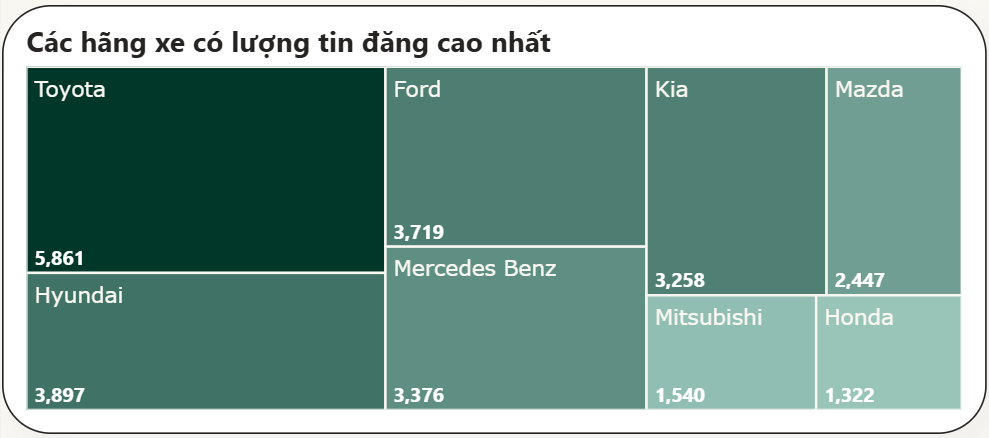
\includegraphics[width=0.8\textwidth]{graphics/Tab01/1.1.png}
\caption{Biểu đồ khối - Treemap Top các hãng xe theo số lượng tin đăng}
\label{fig:tab1_chart_1_1}
\end{figure}

\noindent\textbf{Loại biểu đồ:} Biểu đồ khối - Treemap.

\begin{itemize}
    \item \textbf{Mục đích và ý nghĩa:} Trực quan hóa thị phần tương quan của Top 15 thương hiệu ô tô lớn nhất, giúp người đọc lập tức nhận diện các thương hiệu chi phối thị trường thông qua tỷ lệ diện tích trực quan.
    
    \item \textbf{Sử dụng dữ liệu:}
    \begin{itemize}
        \item Bảng dữ liệu nguồn: \texttt{fact\_car\_listings} kết hợp \texttt{dim\_brand}.
        \item Chỉ số: Đếm số lượng \texttt{Mã tin} nhóm theo \texttt{Tên hãng} (lấy Top 15 thương hiệu hàng đầu).
    \end{itemize}
    
    \item \textbf{Thiết kế và giải thích:} Dạng biểu đồ Treemap phân bố không gian tối ưu cho dữ liệu có nhiều danh mục. Sử dụng một tông màu thuần (Xanh lục đậm) nhất quán để loại bỏ nhiễu thị giác, buộc mắt người xem tập trung trực tiếp vào quy mô diện tích khối.
    
    \item \textbf{Mã hóa trực quan:}
    \begin{itemize}
        \item Kích thước diện tích ô: Tỷ lệ thuận với số lượng tin đăng chào bán của từng hãng xe.
        \item Nhãn thông tin: Hiển thị tên hãng kèm theo số lượng xe và tỷ lệ phần trăm thị phần tương ứng.
    \end{itemize}
    
    \item \textbf{Nhận định và phân tích:}
    \begin{itemize}
        \item Thứ bậc và vị thế thống trị: Toyota vững vàng ở vị trí số 1 với 5.861 tin đăng (chiếm 17,32\% thị phần toàn thị trường), xếp tiếp theo là Hyundai với 3.897 xe (11,51\%) và Ford với 3.719 xe (10,99\%).
        \item Tỷ trọng nhóm dẫn đầu: Top 5 thương hiệu hàng đầu (Toyota, Hyundai, Ford, Mercedes-Benz với 3.376 xe - 9,97\%, và Kia với 3.258 xe - 9,63\%) hợp thành một tập đoàn thống trị chiếm tới 59,42\% tổng lượng xe giao dịch.
        \item Sự hiện diện thương hiệu sang và thương hiệu Việt: Mercedes-Benz là thương hiệu hạng sang duy nhất lọt vào Top 4 thị phần. VinFast - thương hiệu ô tô Việt Nam - đã ghi dấu ấn ở vị trí thứ 11 với 794 xe (chiếm 2,35\% thị phần).
    \end{itemize}
\end{itemize}

% --- Biểu đồ 1.2 ---
\begin{figure}[H]
\centering
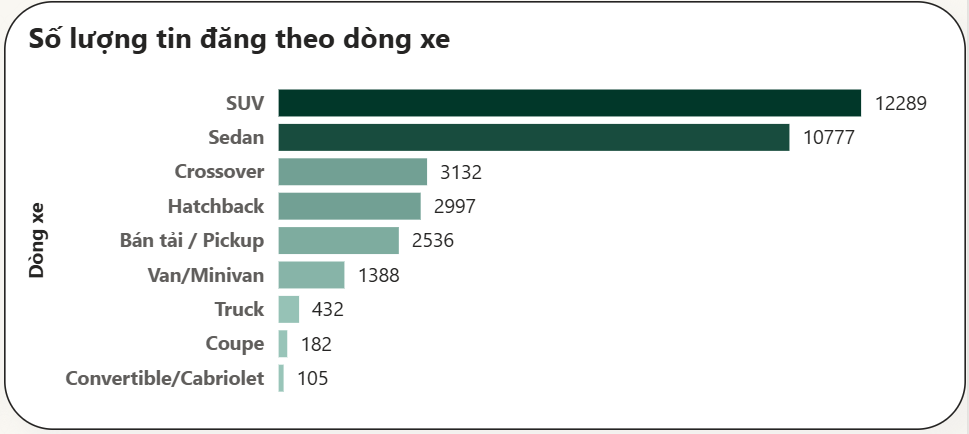
\includegraphics[width=0.8\textwidth]{graphics/Tab01/1.2.png}
\caption{Biểu đồ thanh ngang phân bố số lượng tin đăng theo dòng xe (kiểu dáng thân xe)}
\label{fig:tab1_chart_1_2}
\end{figure}

\noindent\textbf{Loại biểu đồ:} Biểu đồ thanh ngang - Horizontal Bar Chart.

\begin{itemize}
    \item \textbf{Mục đích và ý nghĩa:} Đo lường thị hiếu người tiêu dùng Việt Nam đối với các kiểu dáng thân xe (body type), từ đó xác định xu hướng thiết kế ô tô đang dẫn dắt thị trường.
    
    \item \textbf{Sử dụng dữ liệu:}
    \begin{itemize}
        \item Bảng dữ liệu nguồn: \texttt{fact\_car\_listings} kết hợp \texttt{dim\_body\_type}.
        \item Chỉ số: Đếm số lượng \texttt{Mã tin} nhóm theo \texttt{Tên dòng xe}, xếp hạng giảm dần.
    \end{itemize}
    
    \item \textbf{Thiết kế và giải thích:} Biểu đồ thanh ngang giúp dễ dàng đọc nhãn các kiểu dáng thân xe dài mà không bị che khuất. Các thanh được sắp xếp từ cao xuống thấp tạo cấu trúc trực quan rõ ràng.
    
    \item \textbf{Nhận định và phân tích:}
    \begin{itemize}
        \item Hai trụ cột thị trường: SUV và Sedan tạo thành hai phân khúc áp đảo tuyệt đối. SUV đứng đầu với 12.289 tin đăng (chiếm 36,31\%), theo sát là Sedan với 10.777 tin đăng (chiếm 31,84\%). Tổng cộng hai dòng xe này nắm giữ tới 68,15\% thị phần.
        \item Phân khúc đô thị và đa dụng: Crossover (3.132 xe - 9,25\%) và Hatchback (2.997 xe - 8,85\%) xếp các vị trí tiếp theo, phản ánh nhu cầu di chuyển linh hoạt trong đô thị. Bán tải / Pickup chiếm 2.536 xe (7,49\%) phục vụ nhóm khách hàng thích xe gầm cao cá tính hoặc kinh doanh thương mại.
    \end{itemize}
\end{itemize}

\noindent\textbf{Kết luận và đề xuất hành động cho câu hỏi 1:} 
\begin{itemize}
    \item \textbf{Đúc kết cốt lõi:} Thị trường ô tô Việt Nam có độ tập trung cao vào các thương hiệu phổ thông châu Á (Toyota, Hyundai, Kia) và xe gầm cao (SUV/Crossover) kết hợp Sedan truyền thống.
    \item \textbf{Đề xuất hành động:} 
    \begin{itemize}
        \item \textbf{Đối với đại lý kinh doanh xe:} Tối ưu kho hàng bằng việc tập trung 65 - 70\% nguồn vốn vào các dòng xe SUV và Sedan thuộc Top 5 hãng xe (Toyota, Hyundai, Ford, Kia, Mazda) nhằm đảm bảo tốc độ quay vòng vốn và thanh khoản nhanh nhất.
        \item \textbf{Đối với nhà phân phối / hãng xe mới:} Cần cân nhắc kỹ khi đầu tư vào các phân khúc ngách do thị phần cộng gộp dưới 1\%, thay vào đó nên tập trung vào dải sản phẩm SUV/Crossover cỡ B/C đang rất được ưa chuộng.
    \end{itemize}
\end{itemize}


% ------------------------------------------------------------------------------
% 5.1.4 CÂU HỎI SMART 2
% ------------------------------------------------------------------------------
\subsubsection{Câu hỏi 2}
\label{subsubsec:tab1_q2}

\noindent \textbf{Nội dung câu hỏi: Cấu trúc nguồn cung thị trường được phân bổ như thế nào theo tình trạng phương tiện (Xe cũ vs Xe mới), xuất xứ nguồn cung (Lắp ráp vs Nhập khẩu) và chu kỳ sản xuất (năm sản xuất)?}

% --- Biểu đồ 2.1 ---
\begin{figure}[H]
\centering
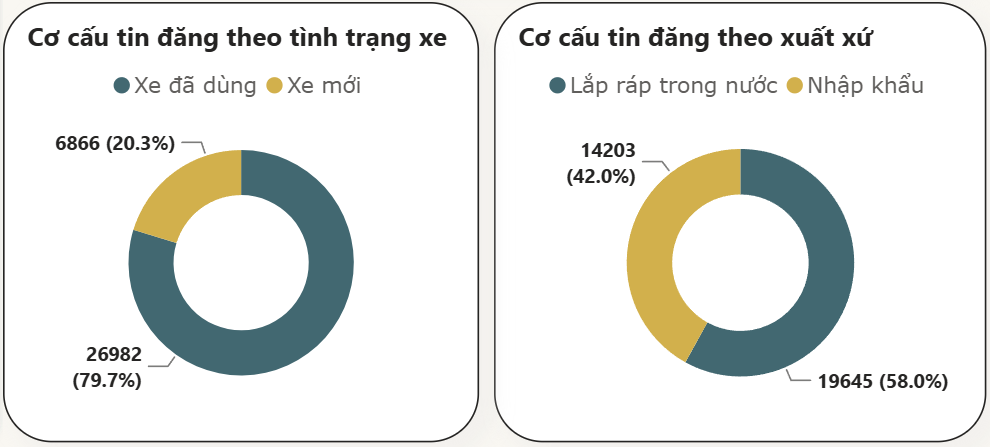
\includegraphics[width=0.8\textwidth]{graphics/Tab01/2.1.png}
\caption{Biểu đồ Donut kép biểu diễn tỷ lệ phân bổ theo Tình trạng và Xuất xứ}
\label{fig:tab1_chart_2_1}
\end{figure}

\noindent\textbf{Loại biểu đồ:} Biểu đồ Donut - Double Donut Charts.

\begin{itemize}
    \item \textbf{Mục đích và ý nghĩa:} So sánh cán cân tỷ lệ giữa xe đã qua sử dụng và xe mới, cũng như cán cân nguồn cung giữa xe lắp ráp trong nước (CKD) và xe nhập khẩu nguyên chiếc (CBU).
    
    \item \textbf{Sử dụng dữ liệu:}
    \begin{itemize}
        \item Bảng dữ liệu nguồn: \texttt{fact\_car\_listings} kết hợp \texttt{dim\_condition} và \texttt{dim\_origin}.
        \item Chỉ số: Tỷ lệ phần trăm tính theo đếm tổng số tin đăng cho các nhóm \texttt{Tình trạng} và \texttt{Xuất xứ}.
    \end{itemize}
    
    \item \textbf{Thiết kế và giải thích:} Biểu đồ Donut kép đặt cạnh nhau giúp người xem dễ dàng đối chiếu hai lát cắt nhị phân quan trọng của thị trường. Nhóm chi phối được phối màu xanh rêu, nhóm phụ phối màu vàng gold.
    
    \item \textbf{Nhận định và phân tích:}
    \begin{itemize}
        \item Về tình trạng xe: Xe đã qua sử dụng (xe cũ) chiếm tỷ trọng áp đảo 79,72\% (với 26.982 tin đăng), trong khi xe mới chỉ chiếm 20,28\% (6.866 tin đăng). Điều này khẳng định sàn giao dịch mang tính chất trọng tâm là thị trường xe cũ thứ cấp.
        \item Về xuất xứ nguồn cung: Xe lắp ráp trong nước (CKD) chiếm ưu thế với 58,04\% (19.645 tin đăng), xe nhập khẩu (CBU) chiếm 41,96\% (14.203 tin đăng). Cán cân này phản ánh năng lực lắp ráp nội địa ngày càng tăng nhờ các chính sách ưu đãi thuế phí của Chính phủ.
    \end{itemize}
\end{itemize}

% --- Biểu đồ 2.2 ---
\begin{figure}[H]
\centering
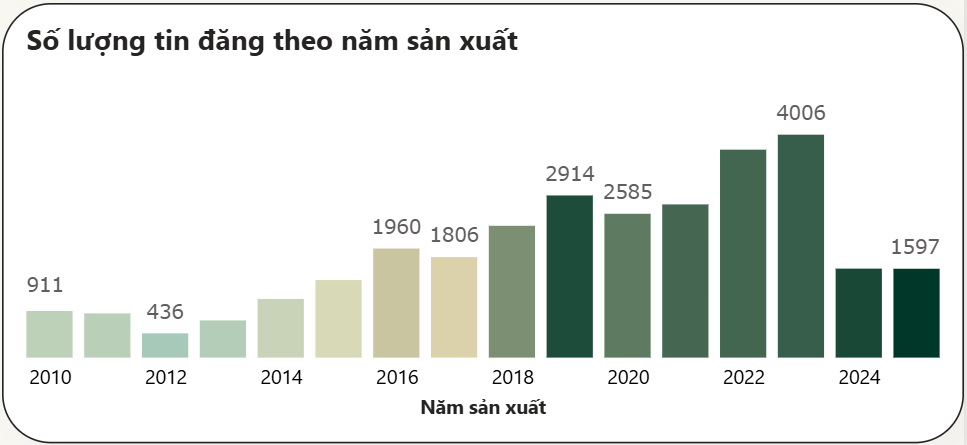
\includegraphics[width=0.8\textwidth]{graphics/Tab01/2.2.png}
\caption{Biểu đồ cột phân bố số lượng xe theo năm sản xuất (1990 - 2025)}
\label{fig:tab1_chart_2_2}
\end{figure}

\noindent\textbf{Loại biểu đồ:} Biểu đồ cột dọc - Column Chart.

\begin{itemize}
    \item \textbf{Mục đích và ý nghĩa:} Đánh giá phân bố tuổi đời xe, xác định chu kỳ thanh lý phổ biến và vùng tập trung mật độ giao dịch cao nhất trên thị trường ô tô.
    
    \item \textbf{Sử dụng dữ liệu:}
    \begin{itemize}
        \item Bảng dữ liệu nguồn: \texttt{fact\_car\_listings}.
        \item Chỉ số: Đếm số lượng xe nhóm theo \texttt{Năm sản xuất} từ 2010 đến 2025.
    \end{itemize}
    
    \item \textbf{Thiết kế và giải thích:} Trục hoành biểu diễn tiến trình thời gian tăng dần, giúp nhận diện rõ sự tích tụ dữ liệu theo chu kỳ sóng.
    
    \item \textbf{Nhận định và phân tích:}
    \begin{itemize}
        \item Vùng tập trung trọng điểm: Dữ liệu phân phối lệch trái mạnh về phía các năm gần đây. Nhóm xe sản xuất từ năm 2020 đến 2025 chiếm tới 48,09\% toàn thị trường (16.277 xe).
        \item Đỉnh sóng thanh lý: Năm sản xuất 2023 có lượng xe giao dịch cao nhất đạt 4.006 xe (11,84\%), theo sau là năm 2022 với 3.737 xe (11,04\%).
        \item Chu kỳ vòng đời: Nhóm xe có tuổi đời từ 5 - 9 năm (sản xuất 2015 - 2019) chiếm 30,85\% (10.443 xe). Các dòng xe đời sâu (sản xuất trước 2015) giảm mạnh chỉ còn chiếm 20,96\% (7.096 xe), chứng tỏ thói quen đổi xe của người tiêu dùng Việt Nam diễn ra mạnh mẽ nhất sau 3 - 6 năm sử dụng.
    \end{itemize}
\end{itemize}

\noindent\textbf{Kết luận và đề xuất hành động cho câu hỏi 2:} 
\begin{itemize}
    \item \textbf{Đúc kết cốt lõi:} Thị trường thứ cấp vận động chủ yếu quanh các dòng xe đời mới (2020-2023), xe đã qua sử dụng 1-4 năm (xe lướt) và xe lắp ráp trong nước.
    \item \textbf{Đề xuất hành động:} 
    \begin{itemize}
        \item \textbf{Đối với người mua xe cũ:} Nên tập trung săn tìm nhóm xe đời 2019 - 2021 (tuổi đời 3-5 năm). Đây là giai đoạn xe đã khấu hao xong phần lớn giá trị ban đầu nhưng chất lượng máy móc và công nghệ vẫn còn rất tốt.
        \item \textbf{Đối với các đơn vị tín dụng / Ngân hàng:} Nên thiết kế các gói vay mua ô tô cũ tập trung cho nhóm xe đời 2020 - 2024 vì rủi ro định giá tài sản đảm bảo thấp và thanh khoản thu hồi nợ cao.
    \end{itemize}
\end{itemize}


% ------------------------------------------------------------------------------
% 5.1.5 TỔNG KẾT VÀ INSIGHT CHIẾN LƯỢC CẤP TAB
% ------------------------------------------------------------------------------
\subsubsection{Tổng kết và định hướng chiến lược cho Tab 1}
\label{subsubsec:tab1_summary}

\noindent\textbf{Tổng hợp các insights chính:}
\begin{itemize}
    \item \textbf{Insight từ câu hỏi 1:} Thị trường mang tính tập trung cao với sự chi phối của Top 5 thương hiệu lớn (Toyota, Hyundai, Ford, Mercedes-Benz, Kia) chiếm gần 60\% lượng tin đăng. SUV và Sedan là hai trụ cột thiết yếu chiếm tới 68,15\% thị phần kiểu dáng.
    \item \textbf{Insight từ câu hỏi 2:} Hơn 79,7\% giao dịch trên thị trường là xe đã qua sử dụng, trong đó gần 50\% tổng lượng xe chào bán có tuổi đời rất mới (sản xuất từ 2020 - 2025). Xe lắp ráp trong nước chiếm ưu thế nguồn cung hơn xe nhập khẩu (58,04\% so với 41,96\%).
\end{itemize}

\noindent\textbf{Trả lời câu hỏi tổng thể:} 
Cấu trúc thị trường ô tô Việt Nam được định hình bởi dòng xe cũ đã qua sử dụng nhưng còn rất mới (xe lướt từ 1 - 5 năm tuổi), chủ yếu là xe lắp ráp trong nước thuộc phân khúc SUV và Sedan của các thương hiệu Nhật Bản và Hàn Quốc. Mức giá trung vị 638 triệu đồng tạo thành ngưỡng ngân sách tiêu chuẩn cho phần đông khách hàng tìm kiếm phương tiện di chuyển cá nhân và gia đình.

\noindent\textbf{Khuyến nghị và hàm ý thực tiễn:}
\begin{itemize}
    \item \textbf{Đối với nhà quản lý \& hoạch định chính sách:} Cần tiếp tục duy trì các chính sách hỗ trợ phát triển ngành công nghiệp phụ trợ ô tô trong nước, do xe lắp ráp CKD hiện đang là trụ cột nguồn cung chính phục vụ nhu cầu đại chúng.
    \item \textbf{Đối với sàn thương mại điện tử / Nền tảng đăng tin:} Cần tối ưu hóa bộ lọc tìm kiếm tập trung vào 3 tiêu chí cốt lõi: Hãng xe (Toyota/Hyundai/Ford), Kiểu dáng (SUV/Sedan) và Năm sản xuất (2020-2024) để giúp người dùng chốt giao dịch nhanh chóng nhất.
\end{itemize}

\subsection{Mục tiêu 2: Phân tích giá xe}
\label{subsec:tab[X]}



% ------------------------------------------------------------------------------
% 5.2.1 BỐI CẢNH VÀ MÔ HÌNH DỮ LIỆU CỦA TAB
% ------------------------------------------------------------------------------
\subsubsection{Bối cảnh phân tích và mô hình dữ liệu}
\label{subsubsec:tab2_schema}

\noindent\textbf{Bối cảnh và mục tiêu phân tích:}
Tab 2: ``Phân tích giá xe'' đóng vai trò trung tâm trong toàn bộ đồ án, trực tiếp trả lời cho bài toán định giá tài sản trên thị trường xe ô tô thứ cấp tại Việt Nam. Tab này giải quyết góc nhìn tài chính, tập trung phân tích cấu trúc phân bổ giá và lượng hóa mức độ tác động của các yếu tố cốt lõi (thương hiệu, tuổi đời, quãng đường sử dụng) lên giá bán. Qua đó, đóng góp vào câu hỏi cốt lõi của đồ án: ``Đâu là mức giá hợp lý và quy luật rớt giá của phương tiện diễn ra như thế nào?''.


{\small
\begin{xltabular}{\textwidth}{L{3cm} L{3.5cm} L{4cm} Y}
\hline
\textbf{Tên cột} & \textbf{Bảng nguồn} & \textbf{Ý nghĩa dữ liệu} & \textbf{Phục vụ phân tích} \\ \hline
\endfirsthead

\multicolumn{4}{l}{\textit{Bảng \thetable{} (tiếp theo)}} \\
\hline
\textbf{Tên cột} & \textbf{Bảng nguồn} & \textbf{Ý nghĩa dữ liệu} & \textbf{Phục vụ phân tích} \\ \hline
\endhead

\hline
\multicolumn{4}{r}{\textit{Còn tiếp ở trang sau}} \\
\endfoot

\hline
\endlastfoot

Mã tin & fact\_car\_listings & Mã định danh duy nhất của mỗi tin đăng bán xe & Biến đo lường (Đếm số lượng) \\
Giá (triệu VND) & fact\_car\_listings & Mức giá chào bán của phương tiện & Biến đo lường (Trung vị, Phân bổ) \\
Năm sản xuất & fact\_car\_listings & Tuổi đời của xe (từ 1990 đến 2025) & Phân loại / Bộ lọc \\
Số Km đã đi sạch & fact\_car\_listings & Quãng đường thực tế xe đã lăn bánh & Phân loại / Trục tọa độ (X) \\
Tên hãng & dim\_brand & Thương hiệu sản xuất (Toyota, Lexus...) & Phân loại / So sánh \\
Tên dòng xe & dim\_body\_type & Kiểu dáng thân xe (Sedan, SUV...) & Bộ lọc (Slicer) \\
\end{xltabular}
}
\begin{center}
\begin{minipage}{\textwidth}
\centering
\captionof{table}{Các trường dữ liệu khai thác}
\label{tab:schema_tab2}
\end{minipage}
\end{center}


% ------------------------------------------------------------------------------
% 5.2.2 KHỐI CHỈ SỐ KPI TỔNG QUAN
% ------------------------------------------------------------------------------
\subsubsection{Khối chỉ số KPI tổng quan}
\label{subsubsec:tab2_kpi}

{\small
\begin{xltabular}{\textwidth}{L{2cm} L{2cm} L{4.5cm} Y}
\hline
\textbf{Thẻ KPI} & \textbf{Giá trị ghi nhận} & \textbf{Công thức hoặc Logic} & \textbf{Ý nghĩa định hướng} \\ \hline
\endfirsthead

\multicolumn{4}{l}{\textit{Bảng \ref{tab:kpi_tab2} (tiếp theo)}} \\
\hline
\textbf{Thẻ KPI} & \textbf{Giá trị ghi nhận} & \textbf{Công thức hoặc Logic} & \textbf{Ý nghĩa định hướng} \\ \hline
\endhead

\hline
\multicolumn{4}{r}{\textit{Còn tiếp ở trang sau}} \\
\endfoot

\hline
\endlastfoot

Tổng số tin đăng & 33.848 & Đếm tổng số dòng dữ liệu hiện có trong bảng fact & Xác định quy mô tập dữ liệu khổng lồ, đảm bảo tính đại diện và độ tin cậy thống kê cho các phép đo lường tiếp theo. \\
Giá trung vị toàn thị trường & 638 triệu & Lấy giá trị median của cột \texttt{Giá (triệu VND)}  & Thiết lập ``mức giá mỏ neo'', đại diện cho ngân sách tiêu chuẩn của phần lớn người mua xe, không bị nhiễu bởi các xe siêu sang. \\
\end{xltabular}
}
\begin{center}
\begin{minipage}{\textwidth}
\centering
\captionof{table}{Các chỉ số KPI điều hướng trên dashboard}
\label{tab:kpi_tab2}
\end{minipage}
\end{center}

% ------------------------------------------------------------------------------
% ------------------------------------------------------------------------------
% 5.2.3 CÂU HỎI SMART 1
% ------------------------------------------------------------------------------
\subsubsection{Câu hỏi 1}
\label{subsubsec:tab2_q1}

\noindent \textbf{Nội dung câu hỏi: Cấu trúc dải giá trên thị trường được phân bổ như thế nào và các thương hiệu siêu sang thiết lập mức giá trần ra sao?}

\begin{figure}[H]
\centering
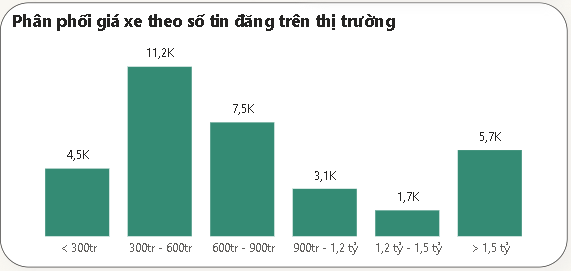
\includegraphics[width=0.8\textwidth]{graphics/Tab02/2.1.PNG}
\caption{Biểu đồ phân phối phân khúc giá xe theo số tin đăng}
\label{fig:tab2_chart_1_1}
\end{figure}

\noindent\textbf{Loại biểu đồ:} Biểu đồ cột dọc.

\begin{itemize}
    \item \textbf{Mục đích và ý nghĩa:} Biểu đồ nhằm xác định phân khúc giá phổ biến nhất, từ đó chứng minh giả thuyết thị trường xe cũ tại Việt Nam chủ yếu được dẫn dắt bởi nhóm khách hàng bình dân và trung lưu.
    
    \item \textbf{Sử dụng dữ liệu:}
    \begin{itemize}
        \item Bảng dữ liệu nguồn: \texttt{fact\_car\_listings}.
        \item Chỉ số: Đếm số lượng \texttt{Mã tin} (Count).
        \item Cột phân nhóm: \texttt{Giá (triệu VND)} (được chia khoảng/bin thành các nhóm: $<$300tr, 300tr - 600tr...).
    \end{itemize}
    
    \item \textbf{Thiết kế và giải thích:} Dạng biểu đồ cột dọc giúp thể hiện trực quan hình dáng phân phối (phân phối lệch phải). Tông màu xanh lục đậm được sử dụng đồng nhất, trong đó cột cao nhất được nhấn mạnh ngầm bằng kích thước áp đảo, điều hướng mắt người xem ngay lập tức vào phân khúc trọng tâm.
    
    \item \textbf{Mã hóa trực quan:}
    \begin{itemize}
        \item Trục ngang (X): Các phân khúc giá tăng dần từ trái sang phải.
        \item Trục dọc (Y): Số lượng tin đăng (K = Nghìn).
        \item Nhãn dữ liệu: Hiển thị trực tiếp con số trên đỉnh mỗi cột (VD: 11,2K) để người đọc không phải gióng sang trục Y.
    \end{itemize}
    
    \item \textbf{Nhận định và phân tích:}
    \begin{itemize}
        \item Thứ bậc và tỷ trọng chính: Phân khúc 300 - 600 triệu đồng chiếm số lượng áp đảo với 11.200 tin đăng, xếp sau là phân khúc 600 - 900 triệu (7.500 tin).
        \item Bối cảnh và lý giải: Đây là tầm giá lý tưởng để mua các dòng xe hạng A, B, C hoặc xe gầm cao đời cũ. Điều này phản ánh thu nhập trung bình và nhu cầu sở hữu ô tô lần đầu của phần lớn các gia đình Việt Nam. 
    \end{itemize}
\end{itemize}

% --- Biểu đồ 1.2 ---
\begin{figure}[H]
\centering
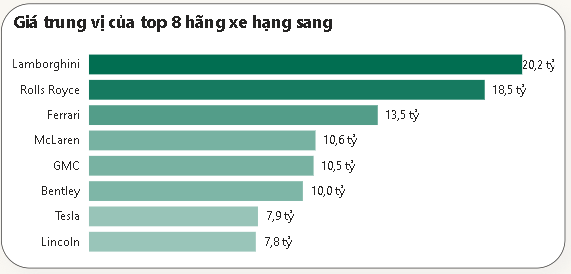
\includegraphics[width=0.8\textwidth]{graphics/Tab02/2.2.PNG}
\caption{Giá trung vị của top 8 hãng xe hạng sang}
\label{fig:tab2_chart_1_2}
\end{figure}

\noindent\textbf{Loại biểu đồ:} Biểu đồ thanh ngang.

\begin{itemize}
    \item \textbf{Mục đích và ý nghĩa:} Mở rộng vào góc khuất cực đoan của thị trường: nhóm xe siêu sang nhằm giúp xác định mức định giá trần mà giới siêu giàu đang chi trả.
    
    \item \textbf{Sử dụng dữ liệu:}
    \begin{itemize}
        \item Bảng dữ liệu nguồn: \texttt{fact\_car\_listings} và \texttt{dim\_brand}.
        \item Chỉ số: Giá trung vị tính từ cột \texttt{Giá (triệu VND)}.
        \item Điều kiện lọc: Chỉ lọc lấy Top 8 hãng xe có giá trị trung vị cao nhất.
    \end{itemize}
    
    \item \textbf{Thiết kế và giải thích:} Biểu đồ thanh ngang giúp dễ dàng đọc tên các hãng xe dài. Ứng dụng kỹ thuật ``Gradient màu'' (nhạt dần từ trên xuống dưới) tạo hiệu ứng thị giác phân cấp mạnh mẽ, tập trung sự chú ý vào hãng xe đắt đỏ nhất.
    
    \item \textbf{Nhận định và phân tích:}
    \begin{itemize}
        \item Thứ bậc và tỷ trọng chính: Lamborghini đứng đầu bảng với mức giá trung vị lên tới 20,2 tỷ đồng, bám sát theo sau là Rolls-Royce với 18,5 tỷ đồng.
        \item Chênh lệch: Có sự ngắt quãng khá rõ giữa Top 3 (trên 13 tỷ) so với phần còn lại của nhóm hạng sang (quanh mốc 10 tỷ).
    \end{itemize}
\end{itemize}

\noindent\textbf{Kết luận và đề xuất hành động cho câu hỏi 1:} 
\begin{itemize}
    \item \textbf{Đúc kết cốt lõi:} Thị trường ô tô Việt Nam phân hóa rất mạnh. Trong khi đại đa số (hơn 50\%) xoay quanh phân khúc bình dân 300 - 900 triệu, thị trường vẫn tồn tại một tầng lớp siêu sang vươn tới mức giá hàng chục tỷ đồng.
    \item \textbf{Đề xuất hành động:} 
    \begin{itemize}
        \item \textbf{Với đại lý bán lẻ:} Nên tập trung tối đa dòng tiền nhập hàng vào phân khúc 300 - 900 triệu vì thanh khoản cao nhất. 
        \item \textbf{Với các nền tảng đăng tin:} Cần có giao diện hoặc khu vực riêng biệt (VIP) để hiển thị nhóm xe siêu sang nhằm thu hút tập khách hàng ngách có tài chính lớn.
    \end{itemize}
\end{itemize}


% ------------------------------------------------------------------------------
% 5.2.4 CÂU HỎI SMART 2
% ------------------------------------------------------------------------------
\subsubsection{Câu hỏi 2}
\label{subsubsec:tab2_q2}
\noindent \textbf{Nội dung câu hỏi: Giá trị của phương tiện khấu hao như thế nào theo tuổi đời (năm sản xuất) và cường độ sử dụng (số kilomet)?}

\begin{figure}[H]
\centering
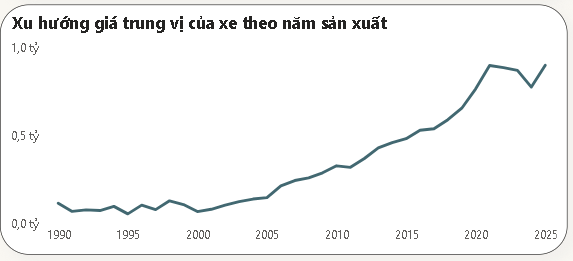
\includegraphics[width=0.8\textwidth]{graphics/Tab02/2.3.PNG}
\caption{Xu hướng biến động giá trung vị của xe theo năm sản xuất (1990 - 2025)}
\label{fig:tab2_chart_2_1}
\end{figure}

\noindent\textbf{Loại biểu đồ:} Biểu đồ đường.

\begin{itemize}
    \item \textbf{Mục đích và ý nghĩa:} Đánh giá độ dốc của sự mất giá phương tiện qua từng năm, giúp trả lời câu hỏi xe giữ giá được bao lâu trước khi chạm đáy khấu hao.
    
    \item \textbf{Sử dụng dữ liệu:}
    \begin{itemize}
        \item Bảng dữ liệu nguồn: \texttt{fact\_car\_listings}.
        \item Chỉ số: Giá trung vị tính từ cột \texttt{Giá (triệu VND)}.
        \item Phân nhóm thời gian (Trục X): \texttt{Năm sản xuất}.
    \end{itemize}
    
    \item \textbf{Thiết kế và giải thích:} Biểu đồ đường là lựa chọn hoàn hảo nhất để quan sát dữ liệu chuỗi thời gian. Đường biểu diễn đậm nét, liên tục, loại bỏ hoàn toàn các đường lưới rối rắm để tối ưu hóa tỷ lệ Data-ink.
    
    \item \textbf{Nhận định và phân tích:}
    \begin{itemize}
        \item Xu hướng: Giá xe rớt dốc cực mạnh ở 5 - 7 năm đầu tiên (từ 2025 lùi về 2018), sau đó đồ thị đi ngang (chạm đáy khấu hao) đối với các xe sản xuất trước năm 2005 (giá chỉ còn dao động dưới 200 triệu).
        \item Bối cảnh: Xe ô tô là tiêu sản. Các công nghệ mới liên tục ra mắt khiến các dòng xe đời cũ nhanh chóng mất đi giá trị ban đầu.
    \end{itemize}
\end{itemize}

% --- Biểu đồ 2.2 ---
\begin{figure}[H]
\centering
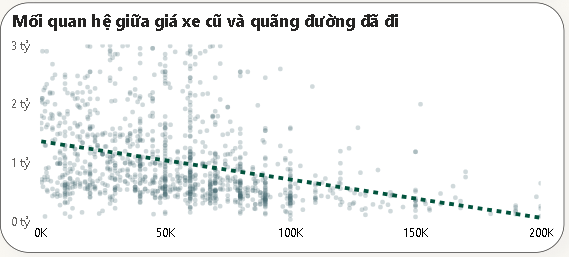
\includegraphics[width=0.8\textwidth]{graphics/Tab02/2.4.PNG}
\caption{Mối quan hệ tương quan giữa giá bán và quãng đường đã di chuyển}
\label{fig:tab2_chart_2_2}
\end{figure}

\noindent\textbf{Loại biểu đồ:} Biểu đồ phân tán kết hợp đường xu hướng.

\begin{itemize}
    \item \textbf{Mục đích và ý nghĩa:} Kiểm chứng mức độ ảnh hưởng của cường độ vận hành (số km thực tế) lên giá bán xe cũ, loại bỏ yếu tố thời gian.
    
    \item \textbf{Sử dụng dữ liệu:}
    \begin{itemize}
        \item Bảng dữ liệu nguồn: \texttt{fact\_car\_listings}.
        \item Trục X: \texttt{Số Km đã đi sạch}.
        \item Trục Y: \texttt{Giá (triệu VND)}.
        \item Điều kiện lọc: Lọc \texttt{Tình trạng} = ``Xe đã dùng'' (chỉ khảo sát xe cũ).
    \end{itemize}
    
    \item \textbf{Thiết kế và giải thích:} Dùng kỹ thuật giảm độ mờ các điểm chấm xuống 30 - 50\% để xử lý tình trạng chồng chéo dữ liệu. Điểm nhấn là đường trendline nét đứt màu đậm cắt ngang đồ thị, chỉ ra rõ rệt hướng đi của dữ liệu.
    
    \item \textbf{Nhận định và phân tích:}
    \begin{itemize}
        \item Xu hướng: Tương quan nghịch biến rõ ràng. Đường xu hướng cắm thẳng xuống từ mốc 0 km đến 200.000 km, xác nhận rằng xe đi càng nhiều, giá trị càng thấp.
        \item Phân tán: Tuy nhiên, các điểm dữ liệu khá vỡ vụn quanh đường xu hướng. Điều này chứng tỏ số Km không phải là yếu tố duy nhất định giá xe (một chiếc xe đi nhiều nhưng hãng sang, bảo dưỡng tốt vẫn có giá cao hơn xe đi ít của hãng giá rẻ).
    \end{itemize}
\end{itemize}

\noindent\textbf{Kết luận và đề xuất hành động cho câu hỏi 2:} 
\begin{itemize}
    \item \textbf{Đúc kết cốt lõi:} Tuổi đời và cường độ khai thác là ``kẻ thù'' lớn nhất bào mòn giá trị ô tô. Đặc biệt, tốc độ mất giá diễn ra tàn khốc nhất trong 5 năm đầu tiên kể từ lúc mua mới.
    \item \textbf{Đề xuất hành động:} 
    \begin{itemize}
        \item \textbf{Với người mua xe cũ:} Nên ưu tiên tìm kiếm những chiếc xe có tuổi đời từ 4 - 6 năm. Đây là thời điểm vàng khi xe đã chịu xong phần khấu hao nặng nề nhất từ chủ cũ nhưng máy móc, công nghệ vẫn còn rất mới.
        \item \textbf{Với người bán (chủ xe):} Nếu muốn tối ưu hóa thu hồi vốn, nên bán xe trước khi chạm mốc 5 năm tuổi hoặc trước khi ODO vượt quá 100.000 km để tránh bị rớt hạng định giá.
    \end{itemize}
\end{itemize}



% ------------------------------------------------------------------------------

% ------------------------------------------------------------------------------
% 5.2.5 TỔNG KẾT VÀ INSIGHT CHIẾN LƯỢC CẤP TAB
% ------------------------------------------------------------------------------
\subsubsection{Tổng kết và định hướng chiến lược cho Tab 2}
\label{subsubsec:tab2_summary}

\noindent\textbf{Tổng hợp các insights chính:}
\begin{itemize}
    \item \textbf{Insight từ câu hỏi 1:} Cấu trúc thị trường phân hóa hình tháp. Đáy tháp cực lớn là phân khúc xe bình dân và trung lưu (dưới 900 triệu đồng) phục vụ nhu cầu đi lại cơ bản. Tuy nhiên, đỉnh tháp lại vươn rất cao với nhóm xe siêu sang (như Lamborghini, Rolls-Royce) chạm mốc trung vị trên 18 tỷ đồng, phục vụ nhu cầu thể hiện đẳng cấp của giới siêu giàu.
    \item \textbf{Insight từ câu hỏi 2:} Xe ô tô là tiêu sản với chu kỳ rớt giá khắc nghiệt. Biểu đồ đường và biểu đồ phân tán cùng chỉ ra rằng: 5 năm đầu tiên và mốc 100.000 km là hai ``ngưỡng cản'' tàn phá giá trị chiếc xe mạnh mẽ nhất, trước khi đồ thị đi ngang và tài sản chạm đáy khấu hao.
\end{itemize}

\noindent\textbf{Trả lời câu hỏi tổng thể:} 
Mức giá hợp lý trên thị trường ô tô Việt Nam xoay quanh mốc trung vị 638 triệu đồng. Mức định giá này không cố định mà bị chi phối mạnh mẽ bởi quy luật khấu hao thời gian và cường độ vận hành. Những chiếc xe lướt (mới sử dụng 1 - 3 năm) chịu mức tổn thất giá trị cao nhất so với giá niêm yết ban đầu, tạo ra khoảng hở chênh lệch lớn mang lại lợi ích cho người mua sau.

\noindent\textbf{Khuyến nghị và hàm ý thực tiễn:}
\begin{itemize}
    \item \textbf{Đối với người mua:} 
    Để tối ưu bài toán kinh tế, tuyệt đối không nên mua xe mới đập hộp nếu ngân sách hạn hẹp. Hãy săn tìm những chiếc xe cũ nằm trong khoảng tối ưu (sản xuất cách đây 4 - 5 năm, ODO dưới 60.000 km) để hưởng trọn phần khấu hao mà chủ cũ đã gánh chịu, trong khi chất lượng xe vẫn còn rất tốt.
    \item \textbf{Đối với người bán:} 
    Nếu có ý định lên đời xe, hãy rao bán phương tiện trước khi nó vượt qua các mốc rớt giá tâm lý nguy hiểm (xe quá 5 năm tuổi hoặc ODO chớm mốc 100.000 km) để có thể thỏa thuận được mức giá hời nhất.
\end{itemize}





\subsection{Mục tiêu 3: Cuộc chiến xe xăng và điện}
\label{subsec:tab3}

% ------------------------------------------------------------------------------
% 5.3.1 BỐI CẢNH VÀ MÔ HÌNH DỮ LIỆU CỦA TAB
% ------------------------------------------------------------------------------
\subsubsection{Bối cảnh phân tích và mô hình dữ liệu}
\label{subsubsec:tab3_schema}

\noindent\textbf{Bối cảnh và mục tiêu phân tích:}
Tab 3 giải quyết một trong những chủ đề nóng nhất của ngành công nghiệp ô tô hiện nay là cuộc cạnh tranh giữa xe sử dụng động cơ đốt trong truyền thống và xe năng lượng mới. Nội dung tập trung làm rõ liệu xe điện chỉ là một trào lưu nhất thời hay thực sự đang định hình lại cấu trúc thị trường. Qua đó, phân tích này đóng góp vào câu hỏi cốt lõi của đồ án bằng cách làm sáng tỏ chiến lược định giá và mức độ tiếp nhận của người tiêu dùng đối với xe năng lượng xanh.

\noindent\textbf{Bảng tổng hợp danh sách trường dữ liệu khai thác:}
\begin{table}[H]
\centering
\small
\begin{tabularx}{\textwidth}{L{3cm} L{3.5cm} L{4.5cm} Y}
\hline
\textbf{Tên cột} & \textbf{Bảng nguồn} & \textbf{Ý nghĩa dữ liệu} & \textbf{Phục vụ phân tích} \\ \hline
Mã tin & fact\_car\_listings & Mã định danh tin đăng bán xe & Biến đo lường (Đếm số lượng) \\ \hline
Nhiên liệu & fact\_car\_listings & Loại năng lượng phương tiện sử dụng (xăng, điện, dầu, hybrid) & Phân loại chính \\ \hline
Năm sản xuất & fact\_car\_listings & Tuổi đời của xe & Phân loại / Trục thời gian \\ \hline
Giá (triệu VND) & fact\_car\_listings & Giá bán của phương tiện & Biến đo lường (Trung vị) \\ \hline
Kiểu dáng & dim\_body\_type & Thiết kế thân xe (SUV, Crossover, Hatchback) & Phân loại (So sánh ngang hàng) \\ \hline
Tình trạng & fact\_car\_listings & Tình trạng sử dụng (Mới, Đã dùng) & Phân loại \\ \hline
Tên hãng & dim\_brand & Thương hiệu sản xuất & Bộ lọc (Đo lường thị phần VinFast) \\ \hline
\end{tabularx}
\caption{Danh sách các trường dữ liệu khai thác trong Tab 3}
\label{tab:schema_tab3}
\end{table}


% ------------------------------------------------------------------------------
% 5.3.2 KHỐI CHỈ SỐ KPI TỔNG QUAN
% ------------------------------------------------------------------------------
\subsubsection{Khối chỉ số KPI tổng quan}
\label{subsubsec:tab3_kpi}

\begin{table}[H]
\centering
\small
\begin{tabularx}{\textwidth}{L{2.5cm} L{2cm} L{4.5cm} Y}
\hline
\textbf{Thẻ KPI} & \textbf{Giá trị} & \textbf{Công thức hoặc Logic} & \textbf{Ý nghĩa định hướng} \\ \hline
Quy mô xe điện & 768 & Đếm tổng số tin đăng lọc theo nhiên liệu là điện & Xác nhận tập dữ liệu mẫu đủ lớn để đưa ra các phân tích thống kê có ý nghĩa, tránh thiên lệch do thiếu dữ liệu. \\ \hline
Thị phần năm 2025 & 19.79\% & Tỷ lệ xe điện trên tổng số xe sản xuất năm 2025 & Cho thấy tốc độ chiếm lĩnh thị trường ở mốc thời gian gần nhất, làm cơ sở để đánh giá xu hướng tương lai. \\ \hline
VinFast dẫn đầu & 89\% & Tỷ lệ xe thuộc hãng VinFast trong tổng số xe điện & Khẳng định vai trò dẫn dắt thị trường và mức độ độc quyền của thương hiệu nội địa trong phân khúc này. \\ \hline
\end{tabularx}
\caption{Tổng hợp các chỉ số KPI điều hướng hàng đầu trên Dashboard Tab 3}
\label{tab:kpi_tab3}
\end{table}

% ------------------------------------------------------------------------------
% 5.3.3 CÂU HỎI SMART 1
% ------------------------------------------------------------------------------
\subsubsection{Câu hỏi 1:}
\noindent \textbf{Nội dung câu hỏi: Xe điện chỉ chiếm 2.3\% toàn bộ dữ liệu - vậy tại sao gọi đây là một “cuộc bứt phá”, và điều gì đang âm thầm xảy ra song song mà ít người để ý?}

\begin{figure}[H]
\centering
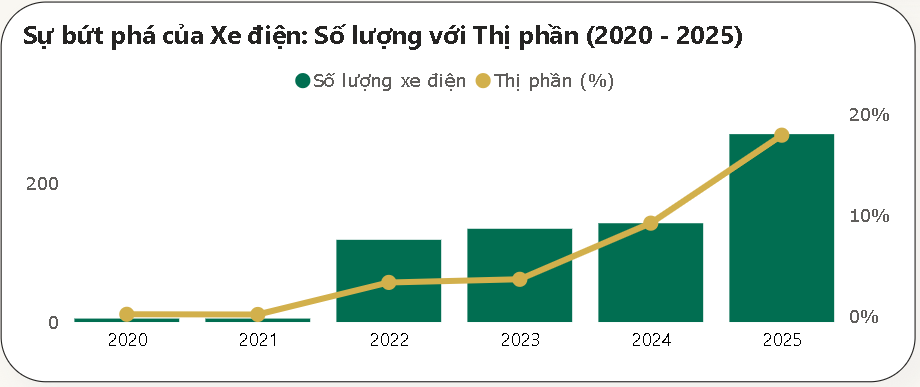
\includegraphics[width=0.8\textwidth]{graphics/Tab03/3.1.PNG}
\caption{Số lượng và thị phần xe điện từ năm 2020 đến 2025}
\label{fig:tab3_chart_5_1}
\end{figure}

\noindent\textbf{Loại biểu đồ:} Biểu đồ kết hợp cột dọc và đường.

\begin{itemize}
    \item \textbf{Mục đích và ý nghĩa:} Biểu đồ giải thích nghịch lý giữa con số tổng lũy kế khiêm tốn (2.3\%) và nhận định về sự bùng nổ của xe điện.
    
    \item \textbf{Sử dụng dữ liệu:}
    \begin{itemize}
        \item Bảng dữ liệu nguồn: \texttt{fact\_car\_listings}.
        \item Chỉ số: Số lượng tin đăng (cột) và tỷ lệ phần trăm (đường).
        \item Điều kiện lọc: Nhiên liệu là điện, năm sản xuất từ 2020 đến 2025.
    \end{itemize}
    
    \item \textbf{Thiết kế và giải thích:} Việc kết hợp cột và đường giúp quan sát đồng thời cả quy mô tuyệt đối lẫn tỷ trọng tương đối. Tông màu xanh lá được sử dụng xuyên suốt để đại diện cho nhóm năng lượng sạch.
    
    \item \textbf{Mã hóa trực quan:}
    \begin{itemize}
        \item Trục ngang: Năm sản xuất tăng dần.
        \item Trục dọc trái: Số lượng xe điện thực tế.
        \item Trục dọc phải: Phần trăm thị phần so với các loại nhiên liệu khác trong cùng năm.
    \end{itemize}
    
    \item \textbf{Nhận định và phân tích:}
    \begin{itemize}
        \item Thứ bậc và xu hướng: Giai đoạn 2020 đến 2021, xe điện gần như vô hình trên bản đồ. Tuy nhiên, từ năm 2022 trở đi, đồ thị đi lên theo chiều dốc đứng. Đến năm 2025, tỷ trọng xe điện đã chạm ngưỡng gần 20\%. 
        \item Bối cảnh và lý giải: Sự bứt phá không nằm ở con số tổng cộng từ quá khứ, mà nằm ở tốc độ tăng trưởng hiện tại. Sự xuất hiện của các dải sản phẩm mới từ thương hiệu nội địa chính là chất xúc tác cho bước nhảy vọt này.
    \end{itemize}
\end{itemize}

\begin{figure}[H]
\centering
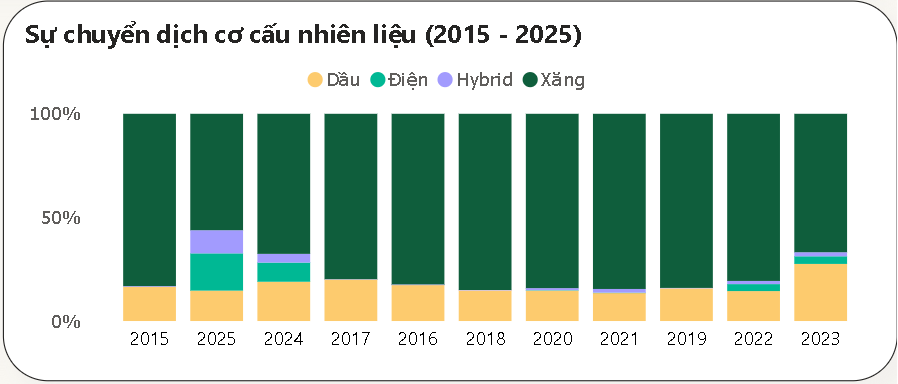
\includegraphics[width=0.8\textwidth]{graphics/Tab03/3.2.PNG}
\caption{Sự chuyển dịch cơ cấu nhiên liệu của thị trường ô tô từ 2015 đến 2025}
\label{fig:tab3_chart_5_2}
\end{figure}

\noindent\textbf{Loại biểu đồ:} Biểu đồ cột chồng 100\%.

\begin{itemize}
    \item \textbf{Mục đích và ý nghĩa:} Trả lời vế sau của câu hỏi bằng cách rõ những thay đổi ngầm trong cơ cấu toàn ngành khi xe điện xuất hiện.
    
    \item \textbf{Sử dụng dữ liệu:}
    \begin{itemize}
        \item Bảng dữ liệu nguồn: \texttt{fact\_car\_listings}.
        \item Chỉ số: Tỷ lệ phần trăm tin đăng.
        \item Phân nhóm: Nhiên liệu (Xăng, Dầu, Hybrid, Điện).
    \end{itemize}
    
    \item \textbf{Thiết kế và giải thích:} Dạng biểu đồ cột chồng 100\% là phương án tối ưu để thấy rõ sự cạnh tranh của thị phần, khi một nhóm tăng lên bắt buộc nhóm khác phải thu hẹp lại.
    
    \item \textbf{Nhận định và phân tích:}
    \begin{itemize}
        \item Sự lấn át: Nhóm xe xăng (màu xanh lục đậm) đang mất dần thế độc tôn từ mốc hơn 80\% ở các năm trước xuống còn tỷ trọng nhỏ hơn hẳn vào năm 2025. 
        \item Diễn biến song song: Đồng hành cùng xe điện, các dòng xe hybrid cũng bắt đầu chiếm một dải mỏng nhưng rõ rệt ở các năm gần đây, minh chứng cho xu hướng người tiêu dùng muốn trải nghiệm điện khí hóa nhưng vẫn cần sự an toàn của động cơ đốt trong.
    \end{itemize}
\end{itemize}

\noindent\textbf{Kết luận và đề xuất hành động cho câu hỏi 1:} 
\begin{itemize}
    \item \textbf{Đúc kết cốt lõi:} Nhìn vào tổng thể toàn bộ lịch sử thị trường thì xe điện vẫn rất bé nhỏ. Tuy nhiên, nếu chỉ tính các xe ra mắt trong ba năm trở lại đây, nhóm xe này đang dần chiếm đi thị phần của xe xăng với tốc độ cực nhanh, đi kèm sự xuất hiện của dòng xe hybrid.
    \item \textbf{Đề xuất hành động:} Các hệ thống garage sửa chữa và dịch vụ bảo dưỡng cần nhanh chóng bổ sung nhân sự và thiết bị chẩn đoán chuyên dụng cho xe điện và hybrid. Nhóm kinh doanh phụ tùng truyền thống sẽ bắt đầu thấy doanh số chững lại trong 3 đến 5 năm tới.
\end{itemize}

% ------------------------------------------------------------------------------
% 5.3.4 CÂU HỎI SMART 2
% ------------------------------------------------------------------------------
\subsubsection{Câu hỏi 2:}
\label{subsubsec:tab3_q6}
\noindent \textbf{Nội dung câu hỏi: Quan niệm phổ biến cho rằng xe điện đắt hơn và được giữ dùng lâu dài, dữ liệu thực tế có xác nhận điều này không?}

\begin{figure}[H]
\centering
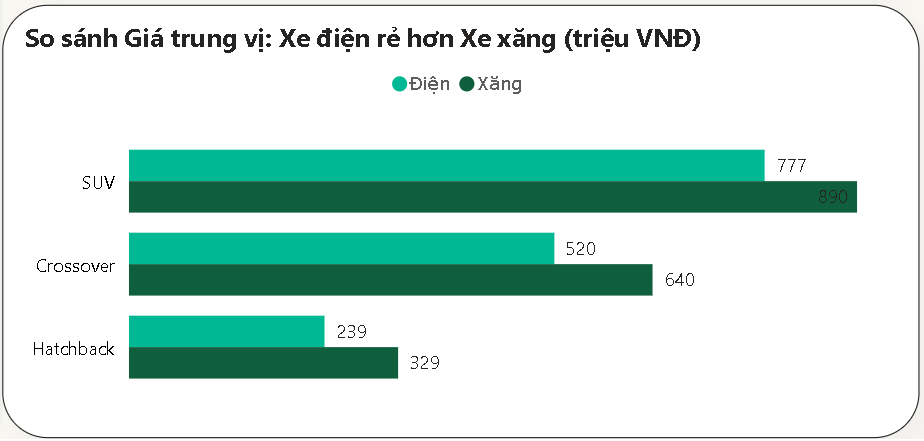
\includegraphics[width=0.8\textwidth]{graphics/Tab03/3.3.PNG}
\caption{So sánh giá trung vị giữa xe điện và xe xăng}
\label{fig:tab3_chart_6_1}
\end{figure}

\noindent\textbf{Loại biểu đồ:} Biểu đồ thanh ngang ghép nhóm.

\begin{itemize}
    \item \textbf{Mục đích và ý nghĩa:} Kiểm chứng định kiến của thị trường cho rằng chi phí sở hữu xe điện luôn cao hơn xe xăng do giá thành pin.
    
    \item \textbf{Sử dụng dữ liệu:}
    \begin{itemize}
        \item Bảng dữ liệu nguồn: \texttt{fact\_car\_listings} và \texttt{dim\_body\_type}.
        \item Chỉ số: Giá trung vị.
        \item Phân nhóm: Nhiên liệu (chỉ lấy Xăng và Điện) và Kiểu dáng (SUV, Crossover, Hatchback).
    \end{itemize}
    
    \item \textbf{Thiết kế và giải thích:} Việc đặt hai thanh ngang cạnh nhau cho từng nhóm kiểu dáng tạo ra sự so sánh trực quan, không qua trung gian.
    
    \item \textbf{Nhận định và phân tích:}
    \begin{itemize}
        \item Chênh lệch giá: Ở mọi phân khúc được khảo sát, giá trung vị của xe điện luôn thấp hơn xe xăng. Điển hình ở phân khúc Hatchback, xe điện có giá trung bình 239 triệu, rẻ hơn rõ rệt so với mức 329 triệu của xe xăng.
        \item Lý giải: Kết quả này phản ánh chính sách định giá mang tính thâm nhập thị trường của nhà sản xuất, kết hợp với các hình thức bán xe không kèm pin giúp giảm chi phí mua ban đầu xuống mức rất dễ tiếp cận.
    \end{itemize}
\end{itemize}

\begin{figure}[H]
\centering
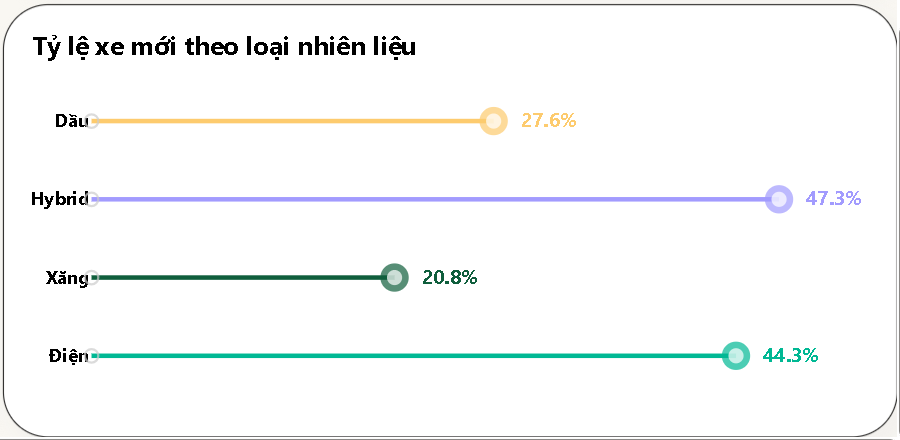
\includegraphics[width=0.8\textwidth]{graphics/Tab03/3.4.PNG}
\caption{Tỷ lệ xe mới được bán theo loại nhiên liệu}
\label{fig:tab3_chart_6_2}
\end{figure}

\noindent\textbf{Loại biểu đồ:} Biểu đồ kẹo mút.

\begin{itemize}
    \item \textbf{Mục đích và ý nghĩa:} Kiểm tra xem người dùng có thực sự giữ xe điện lại để dùng lâu dài như các loại tài sản lớn thông thường hay không.
    
    \item \textbf{Sử dụng dữ liệu:}
    \begin{itemize}
        \item Bảng dữ liệu nguồn: \texttt{fact\_car\_listings}.
        \item Chỉ số: Tỷ lệ phần trăm các tin đăng có Tình trạng là \texttt{mới}.
        \item Phân nhóm: Nhiên liệu.
    \end{itemize}
    
    \item \textbf{Thiết kế và giải thích:} Lược bỏ các cột dày đặc, chỉ giữ lại một thanh mỏng và một điểm tròn có nhãn số liệu, giúp hình ảnh trông thanh thoát hơn và đi thẳng vào kết quả cuối cùng.
    
    \item \textbf{Nhận định và phân tích:}
    \begin{itemize}
        \item Khoảng cách chênh lệch: Lên tới 44.3\% lượng tin đăng xe điện là xe mới chưa lăn bánh, con số này cao gấp đôi so với xe xăng (chỉ 20.8\%). Nhóm hybrid cũng ghi nhận tỷ lệ bán mới rất cao ở mức 47.3\%.
        \item Lý giải: Điều này cho thấy xe năng lượng mới đang có vòng đời đẩy hàng ra thị trường rất nhanh. Lượng lớn tin đăng đến từ các đại lý xả kho hoặc người dùng mua đi bán lại các xe vừa xuất xưởng để chênh lệch giá, phản bác lại quan niệm mua xe điện để gắn bó lâu dài.
    \end{itemize}
\end{itemize}

\noindent\textbf{Kết luận và đề xuất hành động cho câu hỏi 2:} 
\begin{itemize}
    \item \textbf{Đúc kết cốt lõi:} Dữ liệu đã phủ nhận hai định kiến lớn nhất. Xe điện không hề đắt đỏ hơn xe xăng nếu xét cùng phân khúc, và chúng đang tạo ra một xu hướng giao dịch xe mới cực kì sôi động chứ không cố định trong gara của người dùng.
    \item \textbf{Đề xuất hành động:} Người mua có ngân sách hẹp nên cân nhắc chọn xe điện ở phân khúc Hatchback và Crossover để tối ưu chi phí đầu tư. Các nền tảng giao dịch cần tối ưu bộ lọc tìm kiếm xe lướt, xe mới cho nhóm năng lượng này vì nguồn cung đang rất dồi dào.
\end{itemize}

% ------------------------------------------------------------------------------
% 5.3.5 TỔNG KẾT VÀ INSIGHT CHIẾN LƯỢC CẤP TAB
% ------------------------------------------------------------------------------
\subsubsection{Tổng kết và định hướng chiến lược cho Tab 3}
\label{subsubsec:tab3_summary}

\noindent\textbf{Tổng hợp các insights chính:}
\begin{itemize}
    \item \textbf{Insight từ câu hỏi 1:} Xe điện đang tạo ra cú sốc về tốc độ tăng trưởng ở giai đoạn gần đây, âm thầm bóp nghẹt thị phần của xe xăng và kéo theo sự xuất hiện bước đệm của dòng xe lai.
    \item \textbf{Insight từ câu hỏi 2:} Yếu tố cốt lõi giúp xe điện cạnh tranh thành công là chiến lược giá thấp hơn mặt bằng chung, đi kèm với nguồn cung xe mới dồi dào tạo tính thanh khoản cao.
\end{itemize}

\noindent\textbf{Trả lời câu hỏi tổng thể:} 
Cuộc chiến giữa xe xăng và xe điện không còn ở giai đoạn lý thuyết mà đã hiển hiện trên số liệu giao dịch. Xe điện đang sử dụng chiến lược lấy giá cả làm vũ khí mũi nhọn để thay đổi nhận thức người dùng và định hình lại cấu trúc nguồn cung trong tương lai gần.

\noindent\textbf{Khuyến nghị và hàm ý thực tiễn:}
\begin{itemize}
    \item \textbf{Đối với doanh nghiệp và nhà quản lý:} Các đại lý ô tô truyền thống cần đa dạng hóa danh mục nhập hàng, giảm tỷ lệ phụ thuộc vào xe xăng đời mới để tránh tình trạng tồn kho khi làn sóng xe xanh lan rộng. Cần nghiên cứu phát triển thêm mảng dịch vụ thu mua và thẩm định riêng cho pin xe điện.
    \item \textbf{Đối với người mua:} Khách hàng có thể tận dụng lợi thế về giá để trải nghiệm xe điện ở phân khúc phổ thông. Tuy nhiên, do nguồn cung xe mới rất nhiều, người mua cần tham khảo giá kĩ lưỡng để tránh mua hớ ở các đại lý bán lẻ.
\end{itemize}


\subsection{Mục tiêu 4: Chân dung người mua}
\label{subsec:tab[X]}

% ------------------------------------------------------------------------------
% 5.X.1 BỐI CẢNH VÀ MÔ HÌNH DỮ LIỆU CỦA TAB
% ------------------------------------------------------------------------------
\subsubsection{Bối cảnh phân tích và mô hình dữ liệu}
\label{subsubsec:tab4_schema}

\noindent\textbf{Bối cảnh và mục tiêu phân tích:}
Tab 4: ``Chân dung người mua'' tập trung khắc họa thị hiếu và hành vi lựa chọn cấu hình của người tiêu dùng trên thị trường xe ô tô Việt Nam, bao gồm màu sắc ngoại thất, loại hộp số và số chỗ ngồi. Bên cạnh đó, tab còn đối chiếu với hành vi rao bán lại xe cũ thông qua quãng đường đã đi tại thời điểm đăng tin. Qua đó, tab đóng góp vào câu hỏi cốt lõi: ``người mua xe Việt đang ưu tiên cấu hình nào, và thói quen sử dụng xe đã thay đổi ra sao theo thời gian?''.

\begin{table}[H]
\centering
\small
\begin{tabular}{p{3cm} p{3.5cm} p{4cm} p{3.5cm}}
\textbf{Tên cột} & \textbf{Bảng nguồn} & \textbf{Ý nghĩa dữ liệu} & \textbf{Phục vụ phân tích} \\ \hline
Mã tin & fact\_car\_listings & Mã định danh duy nhất của mỗi tin đăng bán xe & Biến đo lường (đếm số lượng) \\
Màu ngoại thất & fact\_car\_listings & Màu sơn bên ngoài xe do người bán khai báo & Phân loại / So sánh tỷ trọng \\
Loại hộp số & fact\_car\_listings & Hình thức truyền động của xe, số tự động hoặc số sàn & Phân loại / Xu hướng theo năm \\
Số chỗ ngồi & fact\_car\_listings & Số lượng ghế ngồi theo thiết kế của xe & Phân loại / Phân bổ tỷ trọng \\
Năm sản xuất & fact\_car\_listings & Năm xe được sản xuất, dùng làm trục thời gian cho xu hướng chuyển dịch hộp số & Trục tọa độ (X) \\
Số Km đã đi sạch & fact\_car\_listings & Quãng đường thực tế xe đã lăn bánh tại thời điểm rao bán lại & Biến đo lường (trung vị) \\
Năm đăng tin & fact\_car\_listings & Thời điểm tin rao bán được đăng lên hệ thống & Trục tọa độ (X) \\
\end{tabular}
\caption{Các trường dữ liệu khai thác}
\label{tab:schema_tab4}
\end{table}

% ------------------------------------------------------------------------------
% khối chỉ số kpi tổng quan
% ------------------------------------------------------------------------------
\subsubsection{Khối chỉ số KPI tổng quan}
\label{subsubsec:tab4_kpi}

\begin{table}[H]
\centering
\small
\begin{tabular}{p{2cm} p{2cm} p{4.5cm} p{5cm}}
\textbf{Thẻ KPI} & \textbf{Giá trị ghi nhận} & \textbf{Công thức hoặc logic} & \textbf{Ý nghĩa định hướng} \\ \hline
Chọn màu trắng & 33,62\% & Tỷ lệ số tin đăng có màu ngoại thất trắng trên tổng số tin đăng & Xác định gu thẩm mỹ chủ đạo của người mua xe Việt, làm cơ sở tham khảo cho đại lý khi nhập hàng theo màu sắc. \\
Chọn số tự động & 82,05\% & Tỷ lệ số tin đăng sử dụng hộp số tự động trên tổng số tin đăng & Cho thấy mức độ phổ biến áp đảo của hộp số tự động, phản ánh sự dịch chuyển thói quen lái xe trong giai đoạn gần đây. \\
Chọn xe 5 chỗ & 68,82\% & Tỷ lệ số tin đăng có cấu hình 5 chỗ ngồi trên tổng số tin đăng & Khẳng định nhu cầu chủ yếu tập trung vào xe cá nhân hoặc gia đình nhỏ, thay vì xe nhiều chỗ phục vụ gia đình lớn hoặc kinh doanh. \\
\end{tabular}
\caption{Các chỉ số KPI điều hướng trên dashboard}
\label{tab:kpi_tab4}
\end{table}
% ------------------------------------------------------------------------------
% 5.X.3 CÂU HỎI SMART 1 (CẤU TRÚC LẶP LẠI CHO Q1, Q2, Q3)
% ------------------------------------------------------------------------------
\subsubsection{Câu hỏi 1}
\label{subsubsec:tab4_q1}

\noindent \textbf{Nội dung câu hỏi: Thị trường ô tô ngày càng đa dạng màu sắc và kiểu dáng, nhưng người mua xe Việt lại ngày càng giống nhau trong lựa chọn, đâu là lý do đằng sau sự đồng nhất bất thường này?}

\begin{figure}[H]
\centering
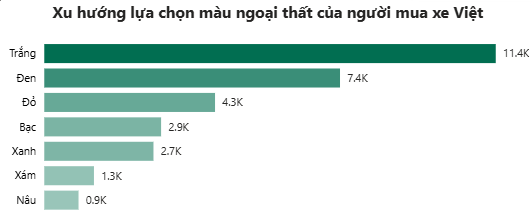
\includegraphics[width=0.8\textwidth]{graphics/Tab04/4.1.PNG}
\caption{Xu hướng lựa chọn màu ngoại thất của người mua xe Việt}
\label{fig:tab4_chart_1_1}
\end{figure}

\noindent\textbf{Loại biểu đồ:} Biểu đồ thanh ngang.

\begin{itemize}
    \item \textbf{Mục đích và ý nghĩa:} Biểu đồ nhằm xác định gu thẩm mỹ chủ đạo của người mua xe Việt, từ đó cung cấp cơ sở tham khảo cho đại lý khi cân đối tỷ trọng màu sắc nhập hàng.
    
    \item \textbf{Sử dụng dữ liệu:}
    \begin{itemize}
        \item Bảng dữ liệu nguồn: \texttt{fact\_car\_listings}.
        \item Chỉ số: Đếm số lượng \texttt{Mã tin} (Count).
        \item Cột phân nhóm: \texttt{Màu ngoại thất}, sắp xếp giảm dần theo số lượng tin đăng.
    \end{itemize}
    
    \item \textbf{Thiết kế và giải thích:} Dạng biểu đồ thanh ngang giúp liệt kê rõ tên các nhóm màu mà không bị chồng chéo nhãn. Tông màu xanh lục được giữ đồng nhất trên toàn bộ các thanh, tránh dùng chính màu sắc thực tế của xe để làm màu biểu đồ vì có thể gây nhiễu thị giác và khó đọc với một số màu nhạt.
    
    \item \textbf{Mã hóa trực quan:}
    \begin{itemize}
        \item Trục dọc (Y): Danh sách các nhóm màu ngoại thất, sắp xếp từ phổ biến nhất đến ít phổ biến nhất.
        \item Trục ngang (X): Số lượng tin đăng tương ứng với mỗi màu.
        \item Nhãn dữ liệu: Hiển thị trực tiếp con số cuối mỗi thanh (VD: 11,4K) để người đọc không phải gióng sang trục X.
    \end{itemize}
    
    \item \textbf{Nhận định và phân tích:}
    \begin{itemize}
        \item Thứ bậc và tỷ trọng chính: Màu trắng dẫn đầu tuyệt đối với 11.400 tin đăng, bỏ xa màu đen ở vị trí thứ hai với 7.400 tin. Nhóm màu trung tính (trắng, đen, bạc, xám) chiếm phần lớn thị phần, trong khi các màu cá tính như đỏ hay xanh chỉ chiếm tỷ trọng nhỏ.
        \item Bối cảnh và lý giải: Xu hướng nghiêng mạnh về màu trung tính phản ánh tâm lý ưu tiên giá trị bán lại và độ trung tính thẩm mỹ khi mua xe tại Việt Nam, thay vì thể hiện cá tính qua màu sắc nổi bật.
        \item Hạn chế: Biểu đồ hiện chỉ thể hiện tỷ trọng tổng gộp toàn bộ giai đoạn, chưa tách theo từng năm nên chưa thể khẳng định mức độ ổn định của thị hiếu màu sắc qua thời gian như câu hỏi đặt ra. Cần bổ sung một biểu đồ xu hướng theo năm sản xuất nếu muốn trả lời trọn vẹn phần này.
    \end{itemize}
\end{itemize}



% ------------------------------------------------------------------------------
% 5.X.4 CÂU HỎI SMART 2
% ------------------------------------------------------------------------------
\begin{figure}[H]
\centering
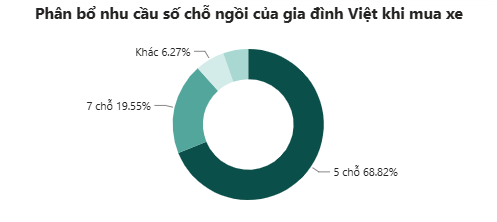
\includegraphics[width=0.8\textwidth]{graphics/Tab04/4.3.PNG}
\caption{Phân bổ nhu cầu số chỗ ngồi của gia đình Việt khi mua xe}
\label{fig:tab4_chart_3_1}
\end{figure}

\noindent\textbf{Loại biểu đồ:} Biểu đồ tròn dạng vành khuyên (donut chart).

\begin{itemize}
    \item \textbf{Mục đích và ý nghĩa:} Biểu đồ nhằm xác định cấu hình số chỗ ngồi chiếm ưu thế trên thị trường, từ đó suy luận nhu cầu sử dụng chủ đạo là xe cá nhân, gia đình nhỏ hay gia đình nhiều thành viên.

    \item \textbf{Sử dụng dữ liệu:}
    \begin{itemize}
        \item Bảng dữ liệu nguồn: \texttt{fact\_car\_listings}.
        \item Chỉ số: Đếm số lượng \texttt{Mã tin}, quy đổi thành tỷ lệ phần trăm trên tổng số tin đăng.
        \item Cột phân nhóm: \texttt{Số chỗ ngồi}, được gom thành các nhóm chính là 5 chỗ, 7 chỗ và khác.
    \end{itemize}

    \item \textbf{Thiết kế và giải thích:} Dạng biểu đồ vành khuyên phù hợp để thể hiện tỷ trọng cấu thành của một tổng thể khi số lượng nhóm phân loại ít. Khoảng trống ở tâm biểu đồ tạo cảm giác nhẹ nhàng hơn so với biểu đồ tròn truyền thống và có thể tận dụng để đặt tổng số tin đăng nếu cần.

    \item \textbf{Mã hóa trực quan:}
    \begin{itemize}
        \item Góc cung: Tỷ lệ phần trăm tương ứng với mỗi nhóm số chỗ ngồi.
        \item Màu sắc: Mỗi nhóm số chỗ ngồi được gán một tông màu xanh riêng biệt, đậm nhạt giảm dần theo tỷ trọng.
        \item Nhãn dữ liệu: Hiển thị trực tiếp tên nhóm và tỷ lệ phần trăm cạnh mỗi phần cung (VD: 5 chỗ 68,82\%).
    \end{itemize}

    \item \textbf{Nhận định và phân tích:}
    \begin{itemize}
        \item Thứ bậc và tỷ trọng chính: Xe 5 chỗ chiếm tỷ trọng áp đảo với 68,82\%, gấp hơn ba lần so với xe 7 chỗ chỉ chiếm 19,55\%, phần còn lại 6,27\% thuộc về các cấu hình khác.
        \item Bối cảnh và lý giải: Tỷ trọng nghiêng mạnh về xe 5 chỗ phản ánh nhu cầu chủ đạo của thị trường vẫn là xe phục vụ cá nhân hoặc gia đình nhỏ, trong khi phân khúc xe 7 chỗ phục vụ gia đình đông thành viên hoặc kinh doanh dịch vụ chỉ chiếm một phần nhỏ.
    \end{itemize}
\end{itemize}

\noindent\textbf{Kết luận và đề xuất hành động cho câu hỏi 1:} 
\begin{itemize}
    \item \textbf{Đúc kết cốt lõi:} Người mua xe Việt Nam đang thể hiện sự đồng nhất bất thường trong 2 lựa chọn tưởng chừng mang tính cá nhân, màu ngoại thất và số chỗ ngồi. Về màu sắc, nhóm màu trung tính (Trắng, Đen) chiếm ưu thế tuyệt đối so với các lựa chọn còn lại. Về cấu hình, nhu cầu tập trung chủ yếu vào xe 5 chỗ phục vụ cá nhân và gia đình nhỏ, trong khi phân khúc nhiều chỗ chỉ giữ vai trò thứ yếu. Cả hai xu hướng cùng phản ánh một tâm lý tiêu dùng thực dụng: người mua đang cân nhắc khả năng thanh khoản khi bán lại và chi phí sử dụng, thay vì thuần túy theo gu thẩm mỹ hay quy mô gia đình lớn.
    \item \textbf{Đề xuất hành động:} 
    \begin{itemize}
        \item \textbf{Với đại lý bán lẻ:} Nên ưu tiên tỷ trọng nhập xe màu trắng và đen ở mức cao nhất vì đây là nhóm có khả năng thanh khoản nhanh nhất, đồng thời duy trì tỷ trọng xe 5 chỗ ở mức cao nhất, chỉ giữ một lượng vừa phải xe 7 chỗ cho nhóm khách hàng gia đình lớn hoặc chạy dịch vụ.
        \item \textbf{Với nhóm phân tích:} Cần bổ sung biểu đồ tách theo năm sản xuất để xác nhận liệu thị hiếu màu trắng có đang tiếp tục tăng hay đã bắt đầu bão hòa, đồng thời có thể tách thêm nhóm 7 chỗ theo dòng xe (SUV, MPV, Van) để hiểu rõ hơn phân khúc này đang phục vụ nhu cầu gia đình hay kinh doanh.
    \end{itemize}
\end{itemize}


\subsubsection{Câu hỏi 2}
\label{subsubsec:tab4_q2}

\noindent \textbf{Nội dung câu hỏi: Điều gì xảy ra khi một thế hệ người mua xe đồng loạt chuyển sang số tự động và cũng đồng loạt bán xe sớm hơn — liệu đây là 2 xu hướng độc lập, hay cùng phản ánh một cách tiêu dùng xe đang thay đổi tận gốc?}

\begin{figure}[H]
\centering
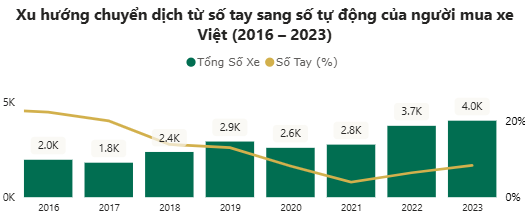
\includegraphics[width=0.8\textwidth]{graphics/Tab04/4.2.PNG}
\caption{Xu hướng chuyển dịch từ số tay sang số tự động của người mua xe Việt (2016 - 2023)}
\label{fig:tab4_chart_2_1}
\end{figure}

\noindent\textbf{Loại biểu đồ:} Biểu đồ kết hợp cột và đường (combo chart).

\begin{itemize}
    \item \textbf{Mục đích và ý nghĩa:} Biểu đồ nhằm lượng hóa tốc độ dịch chuyển công nghệ truyền động, đồng thời đối chiếu quy mô thị trường qua từng năm để tránh nhận định sai lệch khi tỷ lệ phần trăm biến động trên nền số lượng nhỏ.
    
    \item \textbf{Sử dụng dữ liệu:}
    \begin{itemize}
        \item Bảng dữ liệu nguồn: \texttt{fact\_car\_listings}.
        \item Chỉ số cột: Tổng số xe, đếm số lượng \texttt{Mã tin} theo từng năm sản xuất.
        \item Chỉ số đường: Tỷ lệ phần trăm xe số tay trên tổng số xe của năm tương ứng.
        \item Cột phân nhóm: \texttt{Năm sản xuất} (2016 đến 2023), \texttt{Loại hộp số}.
    \end{itemize}
    
    \item \textbf{Thiết kế và giải thích:} Kết hợp cột và đường trên cùng một biểu đồ giúp thể hiện đồng thời hai chiều thông tin, quy mô tuyệt đối (cột) và tỷ trọng tương đối (đường), mà không cần hai biểu đồ tách rời. Trục phụ bên phải dành riêng cho tỷ lệ phần trăm giúp đường xu hướng không bị nén sát đáy biểu đồ.
    
    \item \textbf{Mã hóa trực quan:}
    \begin{itemize}
        \item Trục ngang (X): Năm sản xuất, từ 2016 đến 2023.
        \item Trục dọc trái (Y1): Tổng số xe (đơn vị nghìn).
        \item Trục dọc phải (Y2): Tỷ lệ phần trăm xe số tay.
        \item Nhãn dữ liệu: Hiển thị trực tiếp giá trị trên mỗi cột (VD: 4,0K năm 2023) để người đọc không phải gióng sang trục Y1.
    \end{itemize}
    
    \item \textbf{Nhận định và phân tích:}
    \begin{itemize}
        \item Thứ bậc và tỷ trọng chính: Tổng số xe tăng dần đều qua các năm, từ 2,0K năm 2016 lên 4,0K năm 2023, cho thấy quy mô nguồn cung xe đời mới trên hệ thống ngày càng lớn.
        \item Xu hướng đường tỷ lệ số tay: Đường tỷ lệ xe số tay có xu hướng giảm dần theo thời gian, phản ánh việc hộp số tự động ngày càng chiếm ưu thế trong các đời xe sản xuất gần đây.
        \item Hạn chế: Biểu đồ hiện chưa gắn nhãn phần trăm cụ thể tại từng điểm trên đường xu hướng, khiến việc đọc chính xác mức độ dịch chuyển giữa các năm gặp khó khăn, và cũng chưa tách theo hãng xe để so sánh tốc độ chuyển đổi giữa các thương hiệu.
    \end{itemize}
\end{itemize}



\begin{figure}[H]
\centering
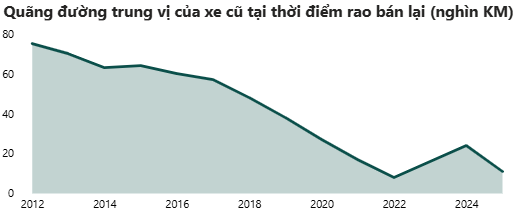
\includegraphics[width=0.8\textwidth]{graphics/Tab04/4.4.PNG}
\caption{Quãng đường trung vị của xe cũ tại thời điểm rao bán lại}
\label{fig:tab4_chart_4_1}
\end{figure}

\noindent\textbf{Loại biểu đồ:} Biểu đồ vùng (area chart).

\begin{itemize}
    \item \textbf{Mục đích và ý nghĩa:} Biểu đồ nhằm theo dõi diễn biến quãng đường trung vị của xe cũ khi được rao bán lại qua từng năm, từ đó suy luận xu hướng nắm giữ hoặc bán lại xe của người dùng đang thay đổi ra sao.

    \item \textbf{Sử dụng dữ liệu:}
    \begin{itemize}
        \item Bảng dữ liệu nguồn: \texttt{fact\_car\_listings}.
        \item Chỉ số: Giá trị trung vị của cột \texttt{Số Km đã đi sạch}.
        \item Cột phân nhóm: \texttt{Năm đăng tin}, trải dài từ 2012 đến 2024.
    \end{itemize}

    \item \textbf{Thiết kế và giải thích:} Dạng biểu đồ vùng giúp nhấn mạnh khối lượng và chiều hướng biến động theo thời gian, phần diện tích tô màu bên dưới đường xu hướng tạo cảm giác trực quan về mức độ suy giảm hay tăng trưởng qua các giai đoạn.

    \item \textbf{Mã hóa trực quan:}
    \begin{itemize}
        \item Trục ngang (X): Năm đăng tin, từ 2012 đến 2024.
        \item Trục dọc (Y): Quãng đường trung vị, đơn vị nghìn km.
        \item Vùng tô màu: Thể hiện giá trị quãng đường trung vị tại mỗi năm, tông xanh nhạt dần khi giá trị giảm.
    \end{itemize}

    \item \textbf{Nhận định và phân tích:}
    \begin{itemize}
        \item Thứ bậc và tỷ trọng chính: Quãng đường trung vị giảm liên tục từ mức khoảng 75 nghìn km năm 2012 xuống mức thấp nhất khoảng 10 nghìn km vào năm 2022, sau đó nhích nhẹ trở lại quanh mốc 20 nghìn km ở các năm gần đây.
        \item Bối cảnh và lý giải: Xu hướng giảm dần cho thấy người dùng có khuynh hướng rao bán lại xe sớm hơn so với trước đây, khi quãng đường đã đi tại thời điểm bán ngày càng thấp, phản ánh chu kỳ nâng đời xe nhanh hơn hoặc tâm lý giữ xe giá trị bán lại cao.
        \item Hạn chế: Đoạn dữ liệu giai đoạn 2022 đến 2023 xuất hiện độ sụt bất thường gần về 0, nhiều khả năng do thiếu dữ liệu hoặc lỗi xử lý outlier, cần rà soát lại trước khi đưa vào kết luận chính thức.
    \end{itemize}
\end{itemize}

\noindent\textbf{Kết luận và đề xuất hành động cho câu hỏi 2:} 
\begin{itemize}
    \item \textbf{Đúc kết cốt lõi:} Hộp số tự động đang dần khẳng định vị thế chủ đạo trên các đời xe sản xuất gần đây, song song với việc quy mô thị trường xe đời mới cũng liên tục mở rộng. Đồng thời, người dùng có xu hướng rao bán lại xe sớm hơn qua từng năm, thể hiện qua quãng đường trung vị giảm dần theo năm sản xuất — cho thấy chu kỳ sở hữu xe đang được rút ngắn. Hai xu hướng này cùng phản ánh một sự dịch chuyển sâu hơn trong thói quen tiêu dùng: người mua xe Việt ngày càng ưu tiên sự tiện dụng tức thời và vòng đời sở hữu ngắn hơn, thay vì gắn bó lâu dài với một chiếc xe như thế hệ trước.
    \item \textbf{Đề xuất hành động:} 
    \begin{itemize}
        \item \textbf{Với đại lý bán lẻ:} Nên ưu tiên nhập các đời xe số tự động cho phân khúc xe đời mới, đồng thời vẫn giữ một tỷ trọng nhỏ xe số sàn cho nhóm khách hàng phổ thông hoặc xe thương mại. Song song đó, cần chú trọng thu mua và tân trang nhóm xe cũ có quãng đường thấp vì đây là nguồn hàng ngày càng phổ biến và dễ bán lại.
        \item \textbf{Với nhóm phân tích:} Nên bổ sung nhãn phần trăm trực tiếp trên đường xu hướng hộp số và tách thêm theo hãng xe để làm rõ hãng nào đang dẫn đầu quá trình chuyển đổi công nghệ truyền động. Đồng thời, có thể đối chiếu quãng đường xe cũ với giá bán để xác nhận liệu xe có quãng đường thấp có thực sự bán được giá tốt hơn hay không.
    \end{itemize}
\end{itemize}
% ------------------------------------------------------------------------------
% 5.X.6 TỔNG KẾT VÀ INSIGHT CHIẾN LƯỢC CẤP TAB
% ------------------------------------------------------------------------------
\subsubsection{Tổng kết và định hướng chiến lược cho tab 4}
\label{subsubsec:tab4_summary}

\noindent\textbf{Tổng hợp các insights chính:}
\begin{itemize}
    \item \textbf{Insight từ câu hỏi 1:} Người mua xe Việt Nam thể hiện sự đồng nhất bất thường trong 2 lựa chọn tưởng chừng mang tính cá nhân — màu ngoại thất và số chỗ ngồi. Nhóm màu trung tính (Trắng, Đen) chiếm tỷ trọng áp đảo so với các màu còn lại, trong khi nhu cầu về cấu hình tập trung chủ yếu vào xe 5 chỗ phục vụ cá nhân và gia đình nhỏ, phân khúc nhiều chỗ chỉ giữ vai trò thứ yếu. Cả hai xu hướng cùng phản ánh một tâm lý tiêu dùng thực dụng: người mua ưu tiên khả năng thanh khoản khi bán lại và chi phí sử dụng hơn là gu thẩm mỹ cá nhân hay quy mô gia đình lớn.
    \item \textbf{Insight từ câu hỏi 2:} Hộp số tự động đang dần thay thế số sàn trên các đời xe sản xuất gần đây, song song với việc quy mô nguồn cung xe đời mới liên tục mở rộng qua từng năm. Đồng thời, quãng đường trung vị của xe cũ tại thời điểm rao bán lại giảm dần theo năm sản xuất, cho thấy người dùng có xu hướng bán lại xe sớm hơn và chu kỳ sở hữu xe đang được rút ngắn. Hai xu hướng này cùng phản ánh một sự dịch chuyển sâu hơn trong thói quen tiêu dùng: người mua xe Việt ngày càng ưu tiên sự tiện dụng tức thời và vòng đời sở hữu ngắn hơn so với thế hệ trước.
\end{itemize}

\noindent\textbf{Trả lời câu hỏi tổng thể:} Chân dung người mua xe Việt Nam hiện nay nghiêng về sự an toàn và thực dụng, ưu tiên màu sắc trung tính dễ bán lại, hộp số tự động tiện dụng, cấu hình 5 chỗ phù hợp nhu cầu cá nhân hoặc gia đình nhỏ, đồng thời có xu hướng nâng đời hoặc thay xe với chu kỳ ngày càng ngắn hơn so với trước đây.

\noindent\textbf{Khuyến nghị và hàm ý thực tiễn:}
\begin{itemize}
    \item \textbf{Đối với doanh nghiệp và nhà quản lý:} Đại lý nên ưu tiên nhập xe màu trung tính, hộp số tự động và cấu hình 5 chỗ vì đây là nhóm có khả năng thanh khoản nhanh nhất, đồng thời chuẩn bị nguồn hàng thu mua xe cũ quãng đường thấp để đáp ứng chu kỳ thay xe ngày càng nhanh của người tiêu dùng.
    \item \textbf{Đối với người mua:} Người mua xe cũ có thể ưu tiên tìm các xe cấu hình phổ biến (màu trung tính, số tự động, 5 chỗ) để dễ dàng bán lại trong tương lai, đồng thời cân nhắc thời điểm bán xe hợp lý để tối ưu giá trị thu hồi trước khi quãng đường sử dụng tăng quá cao.
\end{itemize}

\subsection{Mục tiêu 5: Góc khuất thị trường}
\label{subsec:tab5}

% ------------------------------------------------------------------------------
% 5.5.1 BOI CANH VA MO HINH DU LIEU CUA TAB
% ------------------------------------------------------------------------------
\subsubsection{Bối cảnh phân tích và mô hình dữ liệu}
\label{subsubsec:tab5_schema}

\noindent\textbf{Bối cảnh và mục tiêu phân tích:}
Bốn tab trước xây dựng bức tranh tổng quát về thị trường theo chiều thị phần, giá cả, nhiên liệu và hành vi người mua. Tab 5 tiếp cận từ một góc khác: thay vì mô tả quy luật chung, tab này đi tìm những điểm dữ liệu nằm ngoài quy luật đó. Phân tích tập trung vào ba nhóm câu hỏi: mức giá thực tế ở hai đầu cực của thị trường là bao nhiêu, biên độ dao động giá trong nội bộ một thương hiệu rộng đến đâu, và liệu có hiện tượng đột biến nguồn cung bất thường nào xảy ra theo thời gian. Câu hỏi tổng thể của tab này là: Những điểm dữ liệu bất thường trên thị trường ô tô Việt Nam tiết lộ điều gì về cấu trúc định giá và chuỗi cung ứng?

\begin{table}[H]
\centering
\small
\begin{tabularx}{\textwidth}{L{3cm} L{3.5cm} L{4cm} Y}
\textbf{Tên cột} & \textbf{Bảng nguồn} & \textbf{Ý nghĩa dữ liệu} & \textbf{Phục vụ phân tích} \\ \hline
Giá (triệu VND) & fact\_car\_listings & Mức giá chào bán của phương tiện & Tính giá cực tiểu, cực đại và biên độ chênh lệch nội bộ theo hãng \\
Số km đã đi sạch & fact\_car\_listings & Quãng đường thực tế xe đã lăn bánh & Xác định nhóm xe chạy nhiều km nhất còn được rao bán \\
Năm sản xuất & fact\_car\_listings & Tuổi đời của xe từ 1990 đến 2025 & Trục thời gian phát hiện đột biến nguồn cung theo năm \\
Tên hãng & dim\_brand & Thương hiệu sản xuất & Phân nhóm để đo biên độ dao động giá nội bộ theo hãng \\
\end{tabularx}
\caption{Các trường dữ liệu khai thác cho Tab 5.}
\label{tab:schema_tab5}
\end{table}

% ------------------------------------------------------------------------------
% 5.5.2 KHOI CHI SO KPI TONG QUAN
% ------------------------------------------------------------------------------
\subsubsection{Khối chỉ số KPI tổng quan}
\label{subsubsec:tab5_kpi}


\begin{table}[H]
\centering
\small
\begin{tabularx}{\textwidth}{L{3.5cm} L{2.5cm} L{4cm} Y}
\textbf{Thẻ KPI} & \textbf{Giá trị ghi nhận} & \textbf{Công thức hoặc logic} & \textbf{Ý nghĩa định hướng} \\ \hline
Xe $>$50k km đắt nhất & 12.980 triệu VND & MAX giá của nhóm xe có ODO $>$ 50.000 km & Cho thấy xe siêu sang vẫn giữ giá trị lớn dù cường độ sử dụng cao \\
Xe chạy nhiều km nhất & 500.000 km & MAX của cột số km đã đi sạch & Xác định giới hạn khấu hao vật lý cao nhất được ghi nhận trên hệ thống \\
Số hãng xe hiếm ($\leq$5 xe) & 33 hãng & Đếm số hãng có tổng tin đăng $\leq$ 5 xe & Định lượng nhóm thương hiệu ngách gần như vô hình trên thị trường \\
Lượng xe Ford (SX 2023) & 1.081 xe & Đếm tổng xe Ford có năm sản xuất 2023 & Cảnh báo điểm đột biến nguồn cung bất thường cần xem xét kỹ \\
\end{tabularx}
\caption{Các chỉ số KPI điều hướng trên dashboard Tab 5.}
\label{tab:kpi_tab5}
\end{table}

% ------------------------------------------------------------------------------
% 5.5.3 CAU HOI SMART 1
% ------------------------------------------------------------------------------
\subsubsection{Câu hỏi 1}
\label{subsubsec:tab5_q1}

\noindent \textbf{Nội dung câu hỏi: Mức giá ở hai đầu cực của thị trường được thiết lập như thế nào, và biên độ chênh lệch giá nội bộ của các thương hiệu hạng sang phân bố ra sao?}

\begin{figure}[H]
\centering
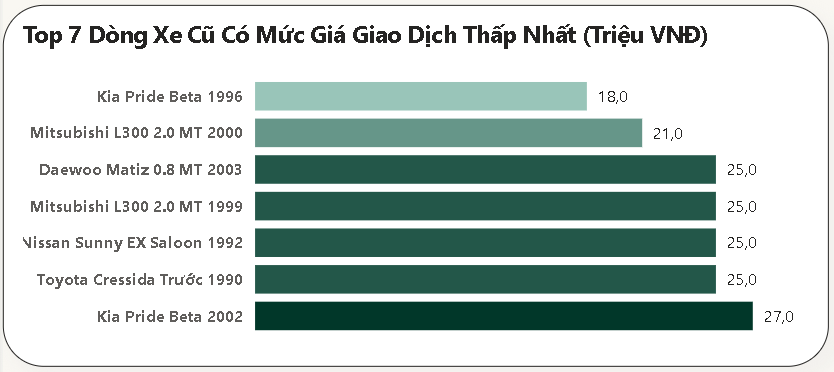
\includegraphics[width=0.95\textwidth]{graphics/Tab05/5.1.PNG}
\caption{Các dòng xe có mức giá thấp nhất thị trường (triệu VND).}
\label{fig:tab5_chart_1}
\end{figure}

\begin{figure}[H]
\centering
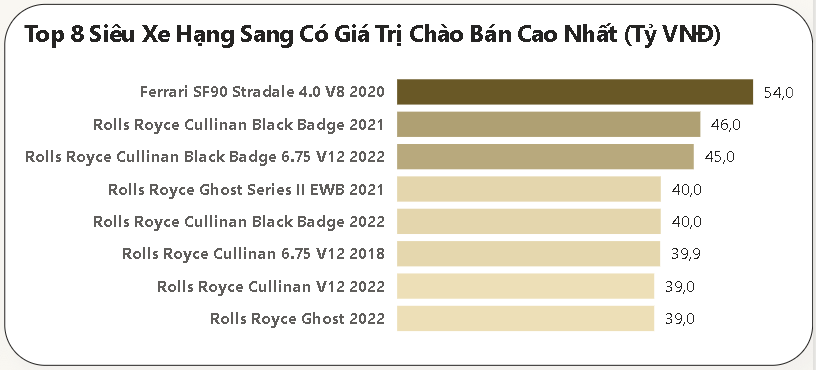
\includegraphics[width=0.95\textwidth]{graphics/Tab05/5.2.PNG}
\caption{Các dòng xe có mức giá cao nhất thị trường (tỷ VND).}
\label{fig:tab5_chart_2}
\end{figure}

\noindent\textbf{Loại biểu đồ:} Biểu đồ thanh ngang, hiển thị hai bảng xếp hạng đặt cạnh nhau.

\begin{itemize}
    \item \textbf{Mục đích và ý nghĩa:} Trực quan hóa đồng thời hai đuôi phân phối giá của thị trường: nhóm xe chạm đáy khấu hao và nhóm xe thiết lập mức giá trần. Đặt hai bảng cạnh nhau giúp khoảng chênh lệch hàng nghìn lần hiện ra ngay lập tức mà không cần thêm chú thích.

    \item \textbf{Sử dụng dữ liệu:}
    \begin{itemize}
        \item Bảng dữ liệu nguồn: \texttt{fact\_car\_listings} kết hợp \texttt{dim\_brand}.
        \item Chỉ số: Cột Giá, lấy theo đơn vị triệu VND ở bảng bên trái và tỷ VND ở bảng bên phải.
        \item Điều kiện lọc: Top 7 dòng xe có giá thấp nhất và Top 8 dòng xe có giá cao nhất.
    \end{itemize}

    \item \textbf{Thiết kế và giải thích:} Biểu đồ thanh ngang được chọn vì tên các phiên bản xe thường dài, cần hiển thị đầy đủ trên nhãn. Hai bảng dùng hai tông màu đối lập, xanh lá cho xe rẻ và nâu vàng cho xe đắt, để phân biệt ngay từ cái nhìn đầu tiên. Thanh được sắp xếp từ giá thấp nhất ở trên, tạo chiều tăng dần từ trên xuống nhất quán ở cả hai bảng.

    \item \textbf{Mã hóa trực quan:}
    \begin{itemize}
        \item Trục ngang (X): Mức giá, đơn vị triệu VND ở bảng bên trái và tỷ VND ở bảng bên phải.
        \item Trục dọc (Y): Tên dòng xe kèm năm sản xuất, sắp xếp tăng dần theo giá từ trên xuống.
        \item Nhãn dữ liệu: Giá trị hiển thị trực tiếp ở cuối mỗi thanh để người đọc không cần gióng sang trục X.
    \end{itemize}

    \item \textbf{Nhận định và phân tích:}
    \begin{itemize}
        \item Đáy thị trường: Mức giá thấp nhất được ghi nhận là 18 triệu VND, thuộc về Kia Pride Beta sản xuất năm 1996. Toàn bộ 7 dòng xe trong danh sách có mức giá từ 18 đến 27 triệu VND, chủ yếu là xe nhỏ và xe tải nhẹ sản xuất trước năm 2005. Đây là nhóm xe đã trải qua hơn hai thập kỷ khấu hao, mức giá thực tế gần như phản ánh giá trị thanh lý phụ tùng hơn là giá trị phương tiện.
        \item Đỉnh thị trường: Ferrari SF90 Stradale 4.0 V8 năm 2020 giữ vị trí cao nhất với 54 tỷ VND, tiếp theo là hai phiên bản Rolls Royce Cullinan Black Badge ở mức 46 và 45 tỷ VND. Đáng chú ý là 7 trong 8 vị trí xe đắt nhất thuộc về Rolls Royce, với các phiên bản dao động từ 39 đến 46 tỷ VND. Lamborghini và Bentley, hai thương hiệu thường được liên tưởng đến mức giá đỉnh, không có mặt trong Top 8 này.
        \item So sánh tổng thể: Khoảng cách giữa chiếc xe rẻ nhất (18 triệu VND) và đắt nhất (54 tỷ VND) lên tới hơn 3.000 lần. Cả hai cùng tồn tại trên một nền tảng rao bán, trong cùng một bộ dữ liệu, phản ánh tính đa dạng cực đoan của hàng hóa ô tô so với hầu hết các loại tài sản tiêu dùng khác.
    \end{itemize}
\end{itemize}

\begin{figure}[H]
\centering
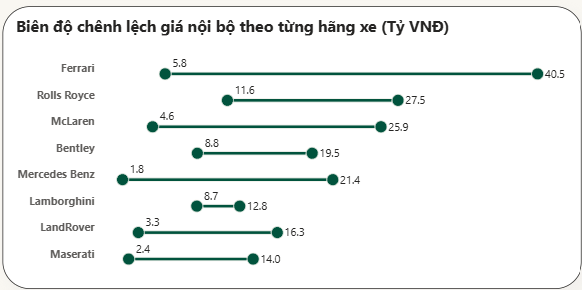
\includegraphics[width=0.95\textwidth]{graphics/Tab05/5.3_Dumbbell.png}
\caption{Biên độ chênh lệch giá nội bộ theo từng hãng xe hạng sang (tỷ VND).}
\label{fig:tab5_chart_3}
\end{figure}

\noindent\textbf{Loại biểu đồ:} Biểu đồ quả tạ.

\begin{itemize}
    \item \textbf{Mục đích và ý nghĩa:} Đo lường biên độ dao động giá trong nội bộ mỗi thương hiệu, trả lời câu hỏi liệu cùng một thương hiệu có thể bán xe ở những mức giá khác nhau đến đâu. Biểu đồ này không hỏi hãng nào đắt hay rẻ mà hỏi hãng nào có khoảng phân tán nội bộ lớn nhất.

    \item \textbf{Sử dụng dữ liệu:}
    \begin{itemize}
        \item Bảng dữ liệu nguồn: \texttt{fact\_car\_listings} kết hợp \texttt{dim\_brand}.
        \item Chỉ số: Với mỗi hãng, tính hai giá trị là biên độ xuống (\texttt{Median} $-$ \texttt{Min}) và biên độ lên (\texttt{Max} $-$ \texttt{Median}), đơn vị tỷ VND.
        \item Điều kiện lọc: Top 8 hãng có tổng biên độ (\texttt{Max} $-$ \texttt{Min}) lớn nhất.
    \end{itemize}

    \item \textbf{Thiết kế và giải thích:} Biểu đồ quả tạ tối ưu tỷ lệ data-ink bằng cách loại bỏ các cột khối nặng nề, chỉ dùng đường nối và hai điểm đầu cuối để truyền tải thông tin về khoảng cách. Điểm bên trái thể hiện biên độ xuống phía giá thấp, điểm bên phải thể hiện biên độ lên phía giá cao. Cách biểu diễn này giúp người đọc so sánh cả độ rộng lẫn vị trí tương đối của mỗi hãng chỉ trong một lượt quan sát.

    \item \textbf{Mã hóa trực quan:}
    \begin{itemize}
        \item Trục ngang (X): Biên độ giá, đơn vị tỷ VND.
        \item Trục dọc (Y): Tên hãng xe, sắp xếp từ tổng biên độ lớn nhất ở trên xuống nhỏ nhất ở dưới.
        \item Điểm marker: Cả hai điểm đầu cuối đều dùng màu xanh đậm. Điểm bên trái thể hiện biên độ xuống (median $-$ min), điểm bên phải thể hiện biên độ lên (max $-$ median). Đường nối màu xanh nhạt hơn thể hiện tổng khoảng phân tán.
        \item Nhãn dữ liệu: Giá trị số ghi trực tiếp cạnh mỗi điểm marker.
    \end{itemize}

    \item \textbf{Nhận định và phân tích:}
    \begin{itemize}
        \item Biên độ lớn nhất: Ferrari dẫn đầu với tổng biên độ 46,3 tỷ VND, trong đó biên độ xuống là 5,8 tỷ và biên độ lên là 40,5 tỷ. Cấu trúc lệch mạnh về phía biên độ lên cho thấy phần lớn xe Ferrari trong dữ liệu tập trung ở vùng giá thấp hơn, trong khi chỉ một số ít phiên bản đẩy trần lên rất cao. Rolls Royce xếp thứ hai với tổng biên độ 39,1 tỷ VND, biên độ xuống 11,6 tỷ và biên độ lên 27,5 tỷ. McLaren đứng thứ ba với tổng biên độ 30,5 tỷ (4,6 và 25,9), tiếp theo là Bentley với 28,3 tỷ (8,8 và 19,5).
        \item Trường hợp đặc biệt của Mercedes Benz: Mercedes có biên độ xuống chỉ 1,8 tỷ VND nhưng biên độ lên tới 21,4 tỷ VND, tổng biên độ 23,2 tỷ. Cấu trúc lệch mạnh này cho thấy giá trung vị của Mercedes nằm rất gần với mức giá thấp nhất của hãng trong dữ liệu, tức phần lớn xe Mercedes thuộc phân khúc tầm trung, trong khi chỉ một nhóm nhỏ phiên bản hiệu năng cao đẩy giá trần lên rất xa so với mặt bằng chung.
        \item Ba hãng còn lại: Lamborghini (8,7 và 12,8, tổng 21,5 tỷ), LandRover (3,3 và 16,3, tổng 19,6 tỷ) và Maserati (2,4 và 14,0, tổng 16,4 tỷ) có tổng biên độ thấp hơn so với nhóm đầu nhưng vẫn phản ánh mức phân tán đáng kể trong nội bộ mỗi hãng. Thứ tự trên biểu đồ phản ánh tổng biên độ tuyệt đối, không phản ánh độ phổ biến hay quy mô thị phần.
    \end{itemize}
\end{itemize}

\noindent\textbf{Kết luận và đề xuất hành động cho câu hỏi 1:}
\begin{itemize}
    \item \textbf{Đúc kết cốt lõi:} Thị trường tồn tại khoảng cách định giá lên tới hơn 3.000 lần giữa xe rẻ nhất và đắt nhất. Thương hiệu không đại diện cho một mức giá cố định mà bao hàm một khoảng phân tán rộng, đặc biệt với nhóm xe hạng sang, nơi mỗi phiên bản và tình trạng xe có thể tạo ra mức giá chênh lệch hàng chục tỷ đồng.
    \item \textbf{Đề xuất hành động:}
    \begin{itemize}
        \item \textbf{Với hệ thống gợi ý sản phẩm:} Khi phân cụm dữ liệu theo khoảng giá, cần phân cụm theo phiên bản và cấu hình cụ thể thay vì gom theo thương hiệu, để tránh gợi ý lệch cho người dùng khi cùng một hãng có thể bán xe ở những mức giá cách nhau vài chục tỷ đồng.
        \item \textbf{Với người mua xe hạng sang:} Cần so sánh kỹ theo phiên bản và năm sản xuất, không nên dùng tên thương hiệu như một đại diện cho mức giá tham chiếu.
    \end{itemize}
\end{itemize}

% ------------------------------------------------------------------------------
% 5.5.4 CAU HOI SMART 2
% ------------------------------------------------------------------------------
\subsubsection{Câu hỏi 2}
\label{subsubsec:tab5_q2}

\noindent \textbf{Nội dung câu hỏi: Có hiện tượng đột biến nguồn cung bất thường nào theo năm sản xuất ở các thương hiệu phổ thông không?}

\begin{figure}[H]
\centering
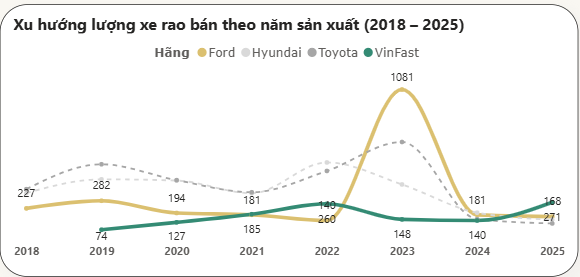
\includegraphics[width=0.95\textwidth]{graphics/Tab05/5.4_LineChart.png}
\caption{Xu hướng lượng xe rao bán theo năm sản xuất của bốn hãng lớn (2018--2025).}
\label{fig:tab5_chart_4}
\end{figure}

\noindent\textbf{Loại biểu đồ:} Biểu đồ đường nhiều chuỗi.

\begin{itemize}
    \item \textbf{Mục đích và ý nghĩa:} Theo dõi diễn biến số lượng xe rao bán theo năm sản xuất của từng hãng, phát hiện các năm có lượng xe đột biến so với xu hướng chung. Biểu đồ này không hỏi tổng số xe là bao nhiêu mà hỏi liệu có hãng nào xuất hiện bất thường tại một thời điểm cụ thể không.

    \item \textbf{Sử dụng dữ liệu:}
    \begin{itemize}
        \item Bảng dữ liệu nguồn: \texttt{fact\_car\_listings} kết hợp \texttt{dim\_brand}.
        \item Trục ngang (X): Năm sản xuất, từ 2018 đến 2025.
        \item Trục dọc (Y): Số lượng xe rao bán, đếm theo số tin đăng.
        \item Chuỗi dữ liệu: Bốn hãng Ford, Hyundai, Toyota và VinFast, được chọn vì có số lượng xe đáng kể và tạo ra các xu hướng đủ để so sánh.
    \end{itemize}

    \item \textbf{Thiết kế và giải thích:} Biểu đồ đường phù hợp nhất để quan sát dữ liệu theo chuỗi thời gian vì nó làm rõ hướng di chuyển và điểm gãy của từng chuỗi. Bốn đường được gán màu khác nhau, trong đó đường Ford màu vàng nổi bật nhất vì đây là chuỗi chứa điểm đột biến cần chú ý. Nhãn số gắn trực tiếp lên từng điểm dữ liệu để người đọc không cần gióng sang trục Y.

    \item \textbf{Mã hóa trực quan:}
    \begin{itemize}
        \item Trục ngang (X): Năm sản xuất 2018 đến 2025, tăng dần từ trái sang phải.
        \item Trục dọc (Y): Số lượng xe, đơn vị chiếc.
        \item Màu sắc: Mỗi hãng một màu riêng biệt, đường Ford màu vàng được phân biệt rõ với ba đường còn lại.
        \item Nhãn dữ liệu: Số lượng cụ thể hiển thị tại mỗi điểm năm trên tất cả các đường.
    \end{itemize}

    \item \textbf{Nhận định và phân tích:}
    \begin{itemize}
        \item Điểm bất thường của Ford năm 2023: Trong khi Hyundai, Toyota và VinFast duy trì lượng xe dao động từ 74 đến 704 chiếc mỗi năm theo xu hướng tương đối ổn định, Ford đột ngột đạt 1.081 chiếc ở nhóm xe sản xuất năm 2023, gấp gần 7,7 lần so với mức 140 chiếc của năm 2022. Đây là mức đột biến lớn nhất trong toàn bộ dữ liệu khi nhìn theo chiều hãng và năm sản xuất.
        \item Trước và sau điểm đột biến: Ford đi vào năm 2023 từ mức 140 chiếc năm 2022 và trở về 181 chiếc năm 2024. Không có chuỗi tăng trưởng dẫn trước để giải thích đỉnh 1.081, cũng không có chuỗi giảm dần sau đó. Đây là dạng đột biến cục bộ, không phải xu hướng kéo dài.
        \item Khả năng lý giải: Dữ liệu không đủ để kết luận nguyên nhân chính xác. Một số khả năng có thể xem xét là lô xe thương mại hoặc xe dịch vụ hết hạn hợp đồng được xả ra cùng lúc, hoặc lô xe lái thử từ hệ thống đại lý được thanh lý đồng loạt. Điều quan trọng là chính việc dữ liệu không tự giải thích được điểm bất thường này là một tín hiệu cần chú ý trong quá trình xây dựng mô hình.
        \item VinFast năm 2025: VinFast đạt 271 chiếc ở nhóm xe sản xuất năm 2025, vượt qua cả Toyota (119 chiếc), Hyundai (146 chiếc) và Ford (168 chiếc) trong cùng năm. Đây là lần đầu tiên VinFast dẫn đầu về số lượng trong nhóm xe đời mới nhất, kết quả nhất quán với xu hướng tăng trưởng thị phần xe điện đã được ghi nhận tại Tab 3.
    \end{itemize}
\end{itemize}

\noindent\textbf{Kết luận và đề xuất hành động cho câu hỏi 2:}
\begin{itemize}
    \item \textbf{Đúc kết cốt lõi:} Nguồn cung trên thị trường không phân phối đồng đều theo thời gian. Trường hợp Ford năm 2023 với 1.081 chiếc là một điểm đột biến cục bộ rõ ràng, không phải xu hướng ổn định. Nếu đưa điểm này vào mô hình học máy mà không xử lý riêng, hệ thống có thể học nhầm phân phối bất thường này là quy luật chung của thị trường Ford.
    \item \textbf{Đề xuất hành động:}
    \begin{itemize}
        \item \textbf{Với nhóm xây dựng mô hình:} Cần gán nhãn và tách riêng tập dữ liệu Ford năm 2023 trước khi huấn luyện bất kỳ mô hình nào liên quan đến dự báo cung hoặc định giá, để tránh mô hình bị ảnh hưởng quá mức bởi một điểm bất thường không đại diện cho xu hướng thực.
        \item \textbf{Với nhóm phân tích:} Nên bổ sung dữ liệu ngoài (ví dụ thông tin từ các đại lý Ford hoặc báo cáo doanh số ngành) để xác minh nguồn gốc của đỉnh 1.081 xe trước khi đưa ra kết luận chính thức.
    \end{itemize}
\end{itemize}

% ------------------------------------------------------------------------------
% 5.5.5 TONG KET VA INSIGHT CHIEN LUOC CAP TAB
% ------------------------------------------------------------------------------
\subsubsection{Tổng kết và định hướng chiến lược cho tab 5}
\label{subsubsec:tab5_summary}

\noindent\textbf{Tổng hợp các Insights chính:}
\begin{itemize}
    \item \textbf{Insight từ câu hỏi 1:} Thị trường có khoảng cách định giá lên tới hơn 3.000 lần giữa xe rẻ nhất (18 triệu VND) và đắt nhất (54 tỷ VND). Các thương hiệu hạng sang có biên độ dao động giá nội bộ rất lớn, trong đó Ferrari dẫn đầu với tổng biên độ 46,3 tỷ VND. Thương hiệu không tương đương với một mức giá cụ thể mà bao hàm một dải phân tán rộng phụ thuộc vào phiên bản và tình trạng xe.
    \item \textbf{Insight từ câu hỏi 2:} Ford sản xuất năm 2023 xuất hiện với 1.081 chiếc, gấp 7,7 lần so với năm trước và trở về mức bình thường ngay sau đó. Đây là điểm bất thường cục bộ về nguồn cung không có giải thích rõ ràng từ dữ liệu. VinFast lần đầu dẫn đầu số lượng xe đời mới năm 2025 với 271 chiếc, vượt qua cả Toyota, Hyundai và Ford trong cùng nhóm năm sản xuất.
\end{itemize}

\noindent\textbf{Trả lời câu hỏi tổng thể:} Thị trường ô tô Việt Nam chứa đựng những điểm dữ liệu bất thường ở cả hai chiều: chiều giá trị tài sản với khoảng phân tán hàng chục tỷ đồng trong cùng một thương hiệu, và chiều cung ứng với các đợt xả hàng đột biến không theo quy luật tăng trưởng thông thường. Những điểm bất thường này không phải nhiễu cần loại bỏ mà là tín hiệu cần được xử lý có chủ đích trước khi đưa dữ liệu vào các bước phân tích tiếp theo.

\noindent\textbf{Khuyến nghị và hàm ý thực tiễn:}
\begin{itemize}
    \item \textbf{Đối với doanh nghiệp và nhà quản lý nền tảng:} Cần thiết lập bộ lọc động để cô lập các tin đăng rơi vào vùng giá cực đoan, tránh làm lệch các báo cáo thống kê trung bình cung cấp cho người dùng phổ thông. Một chiếc xe 54 tỷ đồng nếu được tính vào giá trung vị chung sẽ kéo lệch đáng kể so với thực tế mà đa số người mua tiếp cận.
    \item \textbf{Đối với nhóm xây dựng mô hình dữ liệu:} Trước khi đưa tập dữ liệu này vào huấn luyện hệ thống gợi ý hoặc mô hình dự báo giá, cần xử lý riêng hai nhóm: nhóm xe có giá nằm ngoài khoảng phân vị thứ 5 đến thứ 95 để chuẩn hóa thang đo giá, và nhóm xe Ford năm 2023 để tránh mô hình học nhằm phân phối đột biến không đại diện cho xu hướng thực.
\end{itemize}

\clearpage
\section{Nhận xét và kết luận}

\subsection{Nhận xét tổng hợp}

Đồ án tập trung vào tập \texttt{car\_detail.csv} gồm 30.652 tin đăng xe và 21 cột, phản ánh thị trường xe mới và xe đã dùng tại Việt Nam trong phạm vi năm sản xuất 1990 - 2023. Các thống kê mô tả cho thấy xe đã dùng chiếm tỷ trọng lớn (80,2\%), xe lắp ráp trong nước nhiều hơn xe nhập khẩu (58,3\% so với 41,7\%), hai dòng xe nổi bật nhất là SUV và Sedan, còn Toyota là hãng có số lượng bản ghi cao nhất.

Về kỹ thuật xe, dữ liệu nghiêng mạnh về xe dùng xăng (80,7\%) và hộp số tự động (82,1\%). Số chỗ phổ biến nhất là 5 chỗ, phù hợp với các dòng xe gia đình và đô thị. Dữ liệu cũng tập trung nhiều ở các năm 2018 - 2023, đặc biệt năm 2023 có 4.006 bản ghi, cao nhất trong nhóm năm gần được nêu trong mô tả.

\subsection{Trả lời câu hỏi trung tâm}

Câu hỏi trung tâm của đồ án được xác định là: \textit{``Dữ liệu tin đăng ô tô cho thấy thị trường ô tô Việt Nam được cấu trúc như thế nào về nguồn cung, mức giá và quy luật khấu hao; đồng thời phản ánh ra sao sự chuyển dịch sang xe điện, thị hiếu của người mua và những điểm bất thường cần lưu ý?''}

Dựa trên kết quả của 5 tab phân tích, thị trường trong tập dữ liệu có mức độ tập trung tương đối cao vào một số thương hiệu phổ biến, đặc biệt là Toyota, Hyundai, Ford, Mercedes-Benz và Kia. SUV và Sedan là hai kiểu dáng chủ đạo; xe đã qua sử dụng chiếm phần lớn nguồn cung, trong khi xe lắp ráp trong nước nhỉnh hơn xe nhập khẩu. Mức giá trung vị 638 triệu VND cho thấy phân khúc phổ thông và trung cấp là vùng thị trường trung tâm, mặc dù vẫn tồn tại một nhóm nhỏ xe siêu sang tạo ra khoảng cách rất lớn giữa hai đầu phân phối giá.

Giá trị phương tiện chịu tác động rõ rệt của tuổi đời và quãng đường sử dụng. Giai đoạn khoảng năm năm đầu và ngưỡng 100.000 km là những mốc đáng chú ý, sau đó tốc độ giảm giá có xu hướng chậm lại. Vì vậy, việc định giá xe không thể chỉ dựa trên thương hiệu mà cần kết hợp năm sản xuất, phiên bản, tình trạng và cường độ khai thác thực tế.

Ở chiều chuyển dịch công nghệ, xe xăng vẫn chiếm ưu thế tuyệt đối trong toàn bộ dữ liệu, nhưng xe điện và hybrid tăng nhanh trong nhóm xe đời mới. Xe điện có mức giá cạnh tranh và tỷ lệ xe mới cao, cho thấy quá trình chuyển đổi sang phương tiện năng lượng mới đã bắt đầu thể hiện trên nguồn cung. Về thị hiếu, người mua ưu tiên màu trung tính, hộp số tự động và cấu hình 5 chỗ; quãng đường trung vị của xe cũ khi được rao bán có xu hướng giảm, gợi ý chu kỳ sở hữu và nâng đời xe đang rút ngắn.

Bên cạnh các quy luật chung, dữ liệu còn chứa những điểm cực đoan về giá và đột biến nguồn cung, tiêu biểu là biên độ giá hàng chục tỷ đồng trong cùng một thương hiệu và lượng xe Ford sản xuất năm 2023 tăng bất thường. Các trường hợp này cần được xem là tín hiệu phân tích cần xác minh, thay vì tự động loại bỏ như nhiễu. Như vậy, 5 tab trên dashboard đã tạo thành một mạch phân tích thống nhất: đi từ cấu trúc thị trường, cơ chế định giá, chuyển dịch năng lượng và hành vi người mua đến việc nhận diện các ngoại lệ có thể ảnh hưởng đến quyết định kinh doanh và mô hình dữ liệu.

\subsection{Kết luận và hạn chế}

Báo cáo đã xây dựng được một quy trình phân tích tương đối hoàn chỉnh, từ khảo sát và chuẩn hóa dữ liệu đến tổ chức mô hình và trực quan hóa trên Power BI. Năm tab phân tích bổ sung cho nhau, giúp người xem không chỉ nhận biết nhóm xe và thương hiệu phổ biến mà còn đánh giá mặt bằng giá, quy luật khấu hao, tốc độ thâm nhập của xe điện, thị hiếu cấu hình và các điểm bất thường trong dữ liệu. Kết quả có thể hỗ trợ người mua lựa chọn thời điểm và phân khúc phù hợp, đồng thời cung cấp thông tin tham khảo cho đại lý trong quản lý danh mục và kiểm soát rủi ro định giá.

Tuy nhiên, báo cáo vẫn tồn tại một số hạn chế sau:
\begin{itemize}
    \item \textbf{Phạm vi đại diện của dữ liệu:} Tập dữ liệu được thu thập từ các tin đăng trên một nền tảng trực tuyến nên phản ánh cơ cấu nguồn cung được niêm yết trên nền tảng đó, không đại diện đầy đủ cho toàn bộ thị trường ô tô Việt Nam hoặc các giao dịch ngoại tuyến.
    \item \textbf{Giá chào bán không phải giá giao dịch:} Trường giá thể hiện mức người bán niêm yết, chưa phản ánh giá thương lượng cuối cùng, thời gian bán xe, chi phí sang tên hoặc các ưu đãi đi kèm. Vì vậy, các kết luận về định giá nên được hiểu là phân tích giá chào bán.
    \item \textbf{Các điểm bất thường chưa được xác minh bên ngoài:} Những trường hợp như đột biến nguồn cung xe Ford sản xuất năm 2023 hoặc các mức giá cực đoan mới được phát hiện từ dữ liệu nội bộ. Cần đối chiếu với thông tin đại lý, báo cáo ngành hoặc dữ liệu giao dịch thực tế trước khi diễn giải thành biến động của thị trường.
    \item \textbf{Tính thời điểm của dashboard:} Dashboard phản ánh một ảnh chụp dữ liệu tại thời điểm thu thập và chưa được kết nối với nguồn cập nhật tự động. Các xu hướng và tỷ trọng có thể thay đổi khi bổ sung tin đăng mới hoặc mở rộng sang những nền tảng khác.
\end{itemize}

Trong các nghiên cứu tiếp theo, có thể mở rộng dữ liệu theo thời gian và khu vực, bổ sung giá giao dịch thực tế, thông tin phiên bản và lịch sử xe, đồng thời xây dựng các mô hình dự đoán giá và phát hiện bất thường có bước kiểm định độc lập. Những cải tiến này sẽ giúp dashboard chuyển từ công cụ mô tả sang hệ thống hỗ trợ quyết định có độ tin cậy cao hơn.



\clearpage
% ==============================================================================
% CHƯƠNG: TÍCH HỢP TRÍ TUỆ NHÂN TẠO
% ==============================================================================
\section{Tích hợp trí tuệ nhân tạo}
\label{sec:ai_integration}

% ==============================================================================
% SUBSECTION 1: TỔNG QUAN HỆ THỐNG AI
% ==============================================================================
\subsection{Tổng quan hệ thống AI}
\label{subsec:ai_overview}

\noindent\textbf{Mô tả chung:}
Module AI của đồ án được xây dựng dưới dạng một ứng dụng web độc lập, tích hợp trực tiếp vào tập dữ liệu \texttt{car\_detail.csv} với 33.848 tin đăng xe. Hệ thống cung cấp một giao diện chat cho phép người dùng đặt câu hỏi phân tích bằng ngôn ngữ tự nhiên, yêu cầu AI viết và giải thích đoạn code Python, sau đó tự quyết định có thực thi code đó hay không. Ngoài ra, hệ thống mở Public API để các ứng dụng bên ngoài có thể gọi vào sử dụng.

\noindent\textbf{Vai trò phân công giữa AI và con người:}
\begin{itemize}
    \item \textbf{AI đảm nhận:} Đề xuất hướng phân tích khi người dùng chưa có ý tưởng; tự động sinh code Python/Pandas kèm giải thích bằng ngôn ngữ tự nhiên; trình bày kết quả tính toán dưới dạng bảng Markdown, biểu đồ Matplotlib và câu nhận xét ngắn gọn từ số liệu thực trong tập dữ liệu.
    \item \textbf{Con người đảm nhận:} Đặt ra câu hỏi và hướng phân tích; đọc, chỉnh sửa tham số trong đoạn code AI vừa sinh; ra quyết định có thực thi code hay không; phê duyệt hoặc từ chối các thao tác thay đổi file.
    \item \textbf{Ràng buộc quan trọng:} Code chỉ được chạy trên môi trường local của người dùng. AI không được tự ý thay đổi dữ liệu gốc hay tự sáng tác con số ngoài tập dữ liệu được cung cấp.
\end{itemize}

\noindent\textbf{Công cụ và công nghệ sử dụng:}

% Nhớ đảm bảo \usepackage{xltabular} đã có trong preamble

{\small
\begin{xltabular}{\textwidth}{L{3.8cm} L{3.2cm} Y}
\caption{Công cụ và công nghệ sử dụng trong module AI}
\label{tab:ai_tools} \\
\hline
\textbf{Công cụ / Thư viện} & \textbf{Vai trò} & \textbf{Mô tả sử dụng trong hệ thống} \\ \hline
\endfirsthead

% Cấu hình phần đầu bảng (header) lặp lại khi sang trang mới
\multicolumn{3}{c}%
{{\bfseries Bảng \thetable\ tiếp theo từ trang trước}} \\
\hline
\textbf{Công cụ / Thư viện} & \textbf{Vai trò} & \textbf{Mô tả sử dụng trong hệ thống} \\ \hline
\endhead

% Cấu hình phần chân bảng (footer) ở các trang bị ngắt
\hline \multicolumn{3}{r}{{Tiếp tục ở trang sau...}} \\
\endfoot

% Cấu hình phần chân bảng ở trang cuối cùng
\hline
\endlastfoot

% --- Nội dung bảng ---
FastAPI (Python) & Backend API & Xây dựng ba API bắt buộc: API AI, API Thực thi và API Logs; hỗ trợ streaming SSE để trả lời theo từng token. \\
Next.js (TypeScript) & Frontend & Giao diện chat tương tác, hiển thị code editor có thể chỉnh sửa, card phê duyệt thao tác file và biểu đồ inline. \\
LangChain & Agentic Framework & Quản lý vòng lặp ReAct, liên kết LLM với 15 công cụ, xây dựng lịch sử hội thoại đa lượt. \\
Pandas / NumPy & Tính toán dữ liệu & Thực thi truy vấn phân tích trực tiếp trên DataFrame 33.848 dòng trong bộ nhớ, đảm bảo số liệu từ dữ liệu thực. \\
Matplotlib / Seaborn & Trực quan hóa & Vẽ biểu đồ từ code do AI sinh, tự động encode thành base64 và hiển thị inline trên giao diện chat. \\
Groq / OpenAI / Google / Ollama & Nhà cung cấp LLM & Bốn provider AI có thể hoán đổi từ giao diện quản trị; hỗ trợ cả mô hình đám mây lẫn mô hình local. \\
Playwright + BeautifulSoup & Scraping Agent & Thu thập thông số kỹ thuật và giá xe từ URL người dùng cung cấp, ghi kết quả ra file JSON hoặc CSV. \\
\end{xltabular}
}

\begin{figure}[H]
\centering
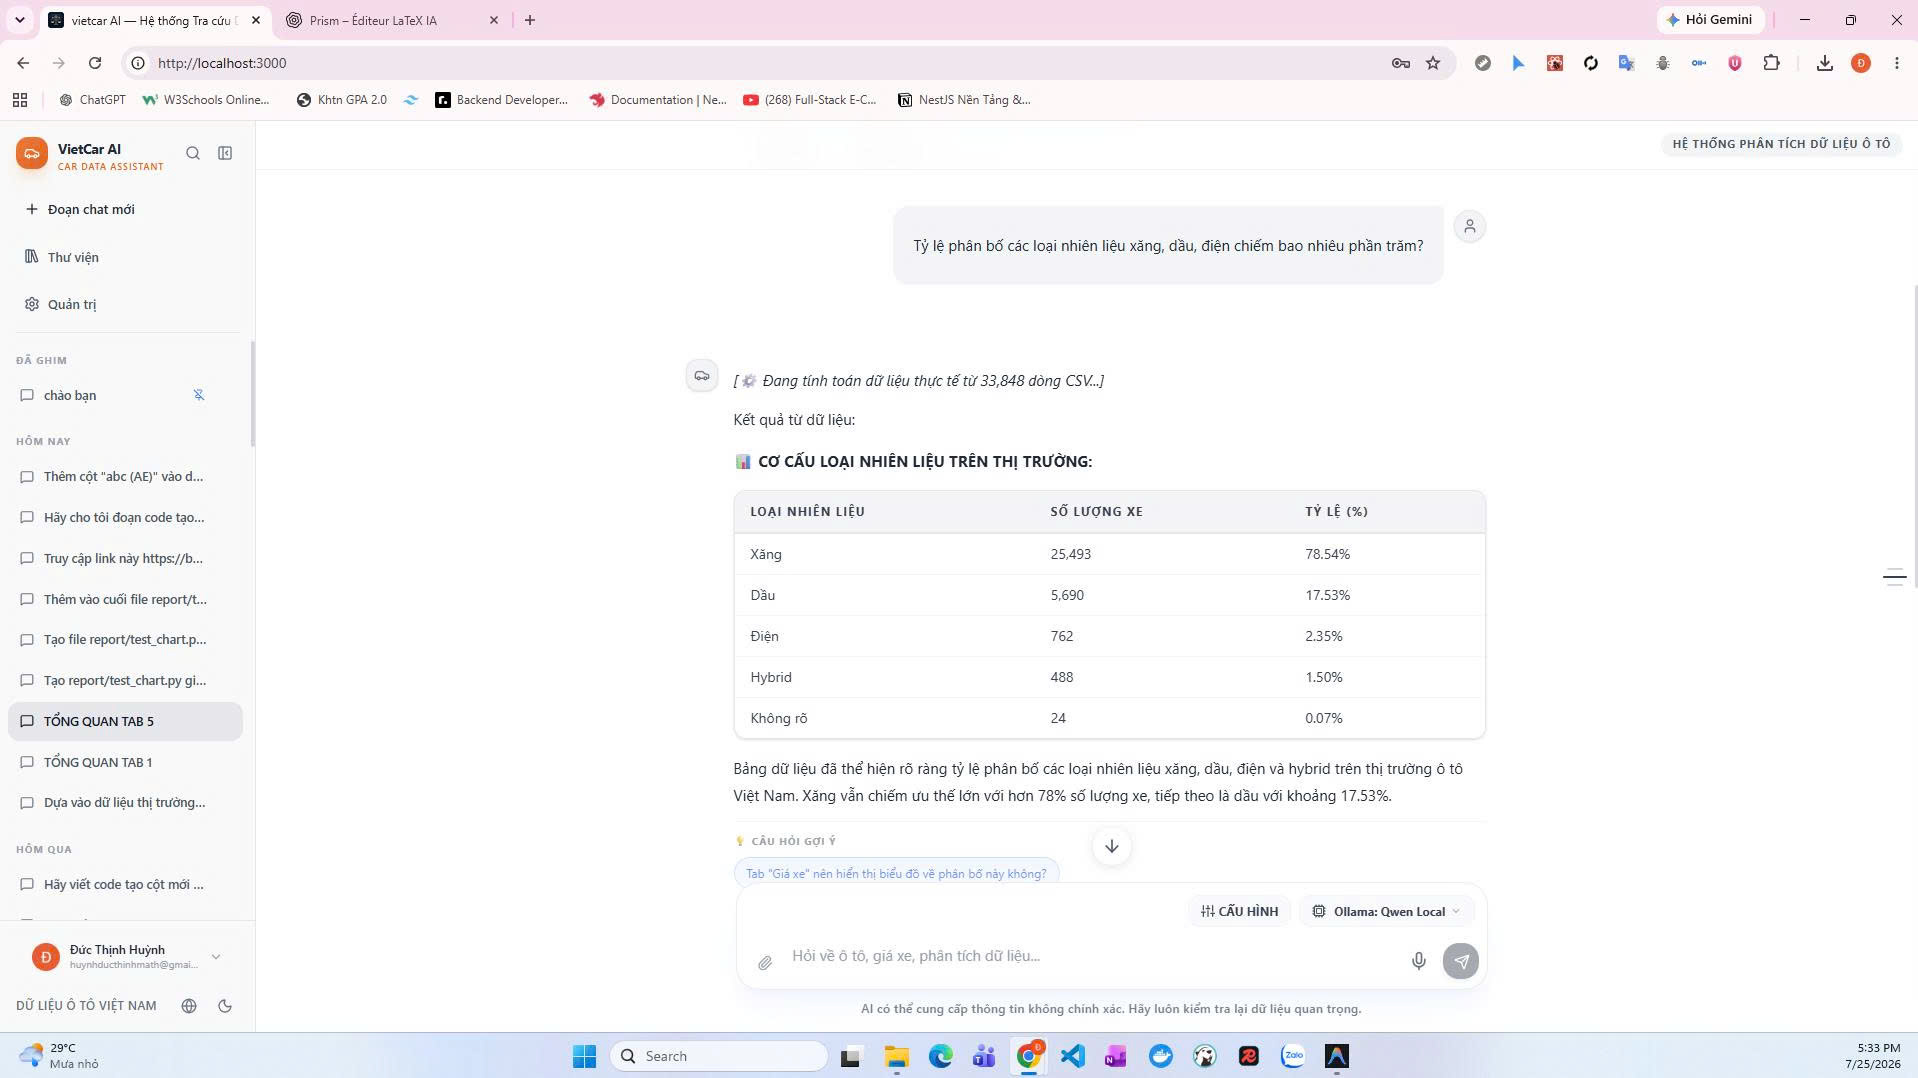
\includegraphics[width=1.00\textwidth]{graphics/AI/ai_overview.jpg}
\caption{Giao diện chính của module AI - ô chat nhận yêu cầu, vùng hiển thị kết quả và lịch sử phiên hội thoại.}
\label{fig:ai_chat_overview}
\end{figure}

% ==============================================================================
% SUBSECTION 2: KIẾN TRÚC KỸ THUẬT
% ==============================================================================
\subsection{Kiến trúc kỹ thuật}
\label{subsec:ai_architecture}

\noindent\textbf{Kiến trúc tổng thể:}
Hệ thống được tổ chức theo mô hình client -- server hai tầng. Tầng Frontend (Next.js, cổng 3000) chịu trách nhiệm thu nhận yêu cầu người dùng và hiển thị kết quả. Tầng Backend (FastAPI, cổng 8000) xử lý toàn bộ logic AI, tính toán dữ liệu và quản lý file, sau đó trả kết quả về Frontend qua giao thức HTTP hoặc SSE Streaming.

\begin{table}[H]
\centering
\small
\begin{tabularx}{\textwidth}{L{3.8cm} L{5.5cm} Y}
\textbf{Router / Module} & \textbf{Endpoint chính} & \textbf{Chức năng} \\ \hline
\texttt{analysis\_chat.py} & \texttt{POST} \newline \texttt{/api/analysis/chat} & API AI: tiếp nhận yêu cầu, gọi LLM kèm ngữ cảnh dữ liệu, streaming SSE từng token. \\
\texttt{execute.py} & \texttt{POST} \newline \texttt{/api/analysis/execute} & API Thực thi: chạy code đã được người dùng phê duyệt, trả về stdout và biểu đồ. \\
\texttt{logs\_analysis.py} & \texttt{POST /log} \newline \texttt{GET /history} & API Logs: lưu và truy xuất lịch sử yêu cầu, code, kết quả theo \texttt{session\_id}. \\
\texttt{file\_operations.py} & \texttt{POST} \newline \texttt{/api/file-operations/} \newline \texttt{\{id\}/approve} & Workflow phê duyệt thao tác file theo từng \texttt{action\_id}. \\
\texttt{public\_api.py} & \texttt{/api/public} & Public endpoint cho ứng dụng bên ngoài gọi vào phân tích dữ liệu. \\
\end{tabularx}
\caption{Danh sách các router backend và chức năng}
\label{tab:ai_routers}
\end{table}

% ------------------------------------------------------------------------------
\subsubsection{API AI (Tiếp nhận yêu cầu và sinh code có giải thích)}
\label{subsubsec:api_ai}

\noindent\textbf{Mô tả chức năng:}
API AI đóng vai trò trung tâm của hệ thống. Khi người dùng gửi một câu hỏi hoặc yêu cầu phân tích, backend không chỉ đơn giản chuyển tiếp tin nhắn đến LLM mà còn đính kèm ngữ cảnh dữ liệu phong phú, giúp mô hình AI hiểu cấu trúc bài toán và giảm khả năng sinh ra thông tin không có trong dữ liệu.

\noindent\textbf{Ngữ cảnh được gửi kèm cho LLM bao gồm:}
\begin{itemize}
    \item \textbf{Schema bộ dữ liệu:} Danh sách 21 cột, kiểu dữ liệu, ý nghĩa nghiệp vụ và thống kê mô tả cơ bản (kích thước, tỷ lệ thiếu).
    \item \textbf{Trạng thái DataFrame hiện tại:} Sau mỗi lần thực thi code, hệ thống ghi lại \texttt{df\_context} (shape, dtypes, null counts) và đưa vào context lần gọi tiếp theo, giúp AI nắm được dữ liệu đang ở trạng thái nào trong phiên làm việc.
    \item \textbf{Lịch sử hội thoại:} Các lượt hỏi đáp trước trong cùng phiên, cho phép người dùng hỏi tiếp nối mà không cần lặp lại bối cảnh.
    \item \textbf{Dữ liệu Dashboard:} Khi câu hỏi liên quan đến các chỉ số KPI hoặc biểu đồ đã có trong dashboard Power BI, hệ thống trích xuất trực tiếp từ \texttt{Dashboard.json} và đưa vào phản hồi mà không cần gọi LLM tính toán lại.
\end{itemize}

\noindent\textbf{Yêu cầu đối với đầu ra của AI:}
\begin{itemize}
    \item Khi AI sinh code Python, đoạn code đó phải được hiển thị rõ ràng trong khối \texttt{InteractiveCodeBlock} trên giao diện, kèm theo đoạn giải thích bằng ngôn ngữ tự nhiên phía trên.
    \item Giải thích phải mô tả cụ thể đoạn code sẽ làm gì (ví dụ: ``Đoạn code dưới đây nhóm dữ liệu theo cột \texttt{Hãng} và tính giá trung vị cho mỗi nhóm, sau đó sắp xếp theo thứ tự giảm dần.'').
    \item AI không được tự ý thêm số liệu hay kết quả phân tích nếu chưa có đoạn code tương ứng được thực thi thành công.
\end{itemize}

% ------------------------------------------------------------------------------
\subsubsection{API Thực thi (Chạy code đã được phê duyệt trên local)}
\label{subsubsec:api_execute}

\noindent\textbf{Mô tả chức năng:}
Sau khi AI sinh ra đoạn code, người dùng có thể đọc, chỉnh sửa và quyết định có thực thi hay không. Khi bấm nút \textbf{Thực thi}, Frontend gửi đoạn code (có thể đã được người dùng sửa đổi so với bản gốc AI sinh ra) lên \texttt{POST /api/analysis/execute}. Backend thực thi code trực tiếp trên dữ liệu tại máy.

\noindent\textbf{Cơ chế namespace bền vững theo phiên:}
\begin{itemize}
    \item Mỗi phiên làm việc (\texttt{session\_id}) được cấp một namespace Python riêng, lưu giữ biến \texttt{df} và các biến khác giữa các lần thực thi. Người dùng không cần load lại dữ liệu ở mỗi câu hỏi mới trong cùng phiên.
    \item Khi phiên kết thúc hoặc hết hạn, namespace được giải phóng để thu hồi bộ nhớ.
\end{itemize}

\noindent\textbf{Xử lý kết quả trả về:}
\begin{itemize}
    \item \textbf{Văn bản (stdout):} Kết quả in ra từ \texttt{print()} hoặc giá trị cuối cùng của biểu thức được trả về và hiển thị trong khung kết quả bên dưới ô code.
    \item \textbf{Biểu đồ (hình ảnh):} Sau khi code chạy xong, hệ thống quét tất cả figure Matplotlib đang mở, encode sang định dạng PNG base64 và nhúng trực tiếp vào giao diện chat mà không cần lưu file ảnh ra đĩa.
    \item \textbf{Lỗi thực thi:} Nếu code gây ra exception, thông báo lỗi được hiển thị rõ ràng để người dùng biết và điều chỉnh.
\end{itemize}

\begin{table}[H]
\centering
\small
\begin{tabularx}{\textwidth}{L{3cm} L{3cm} Y}
\textbf{Tham số gửi lên} & \textbf{Kiểu} & \textbf{Mô tả} \\ \hline
\texttt{code} & string & Đoạn code Python người dùng muốn thực thi (có thể khác với bản AI sinh nếu đã sửa). \\
\texttt{session\_id} & string & Định danh phiên làm việc để hệ thống truy xuất đúng namespace Python tương ứng. \\ \hline
\textbf{Kết quả trả về} & & \\ \hline
\texttt{stdout} & string & Toàn bộ văn bản in ra trong quá trình thực thi. \\
\texttt{images} & list[string] & Danh sách biểu đồ dạng base64 PNG, một phần tử cho mỗi figure Matplotlib. \\
\texttt{error} & string & Thông báo lỗi nếu có exception xảy ra. \\
\texttt{df\_context} & string & Mô tả trạng thái DataFrame sau khi thực thi, được lưu để đưa vào context lần hỏi tiếp theo. \\
\end{tabularx}
\caption{Cấu trúc request và response của API Thực thi}
\label{tab:execute_api}
\end{table}
\begin{figure}[H]
\centering
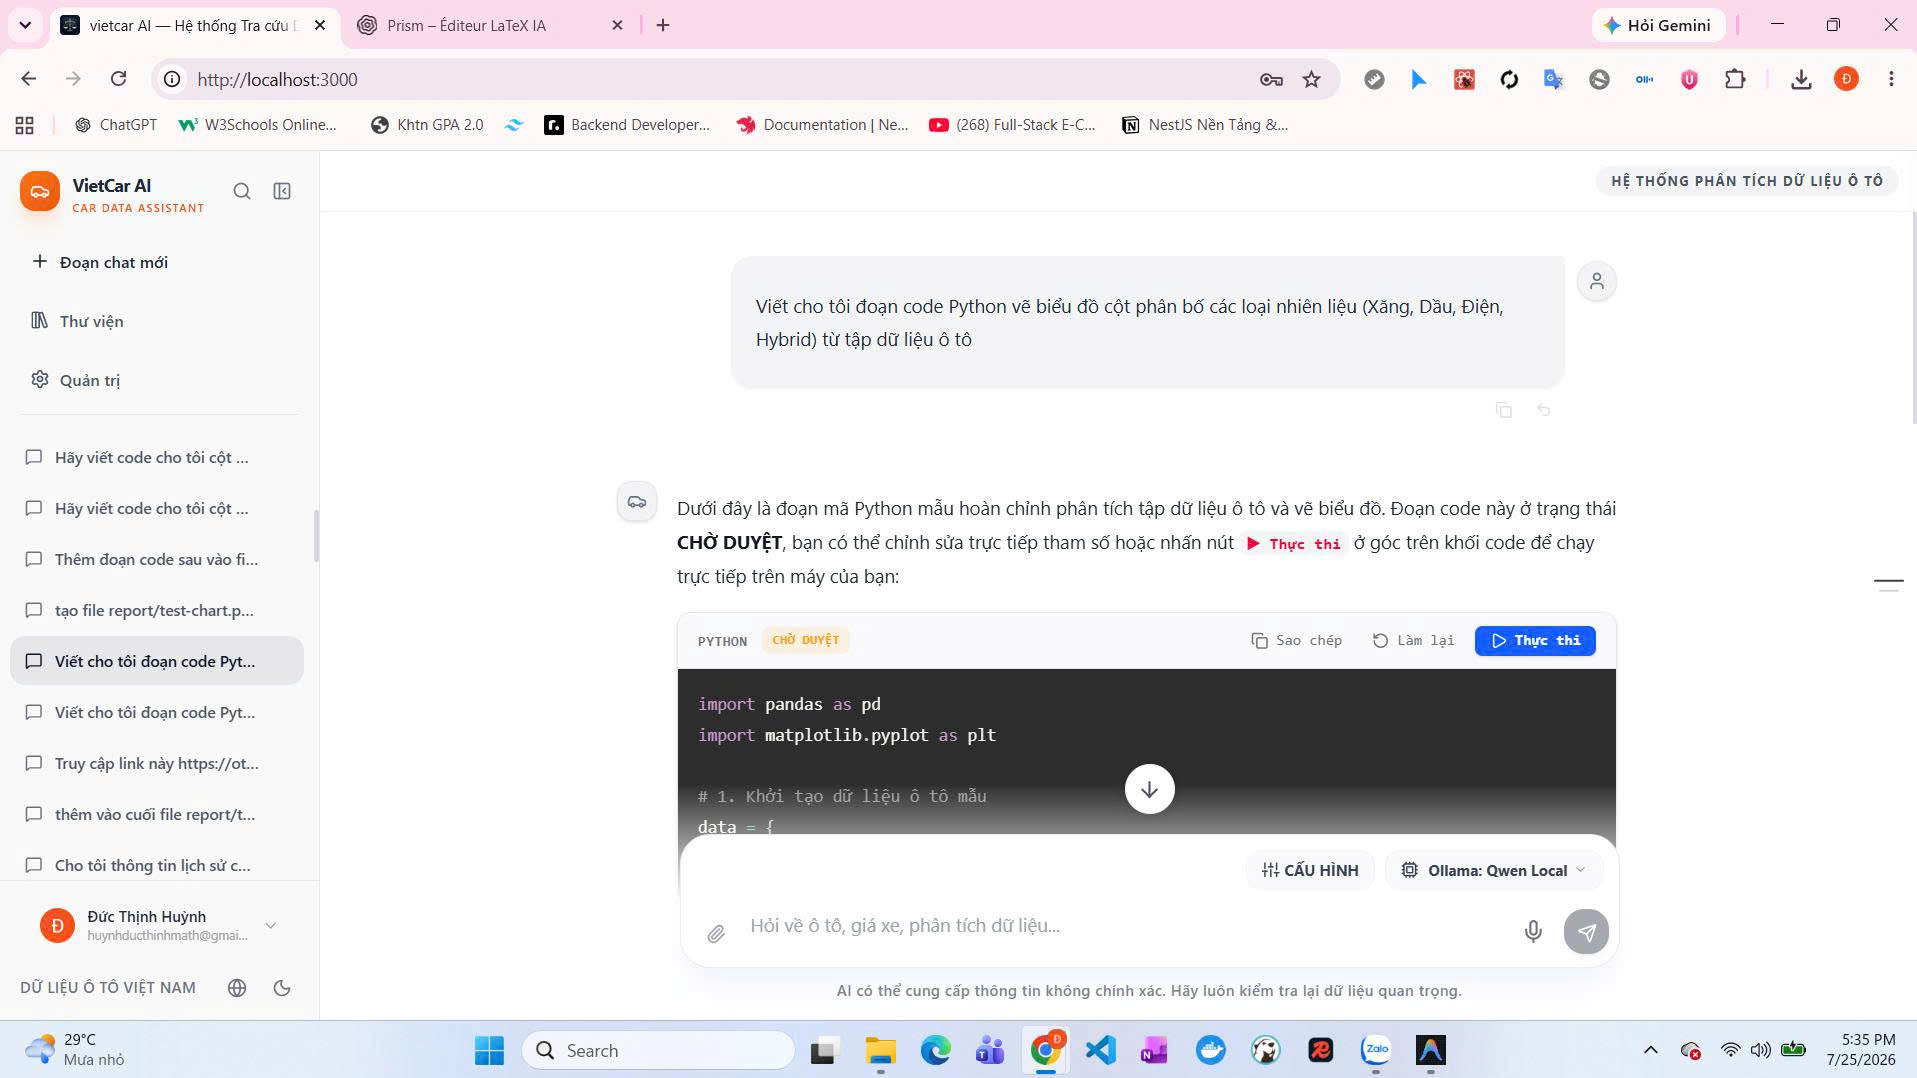
\includegraphics[width=1.00\textwidth]{graphics/AI/ai_tr79.jpg}
\caption{Khối \texttt{InteractiveCodeBlock}: editor code có thể chỉnh sửa ở trên, vùng kết quả bên dưới hiển thị bảng dữ liệu hoặc biểu đồ Matplotlib sau khi bấm Thực thi.}
\label{fig:ai_chat_overview}
\end{figure}


% ------------------------------------------------------------------------------
\subsubsection{API Logs (Lưu trữ yêu cầu, mã nguồn và kết quả)}
\label{subsubsec:api_logs}

\noindent\textbf{Mô tả chức năng:}
Theo nguyên tắc lưu trữ được quy định trong hướng dẫn tích hợp AI, hệ thống ghi lại toàn bộ nhật ký hoạt động vào file \texttt{logs/analysis\_logs.jsonl} ở định dạng JSON Lines.

\noindent\textbf{Thông tin được lưu trong mỗi bản ghi:}
\begin{itemize}
    \item \textbf{Yêu cầu người dùng:} Nội dung câu hỏi hoặc yêu cầu phân tích gốc (\texttt{user\_request}).
    \item \textbf{Mã nguồn:} Đoạn code Python AI sinh ra (\texttt{code}), phản ánh đúng trạng thái cuối cùng trước khi thực thi.
    \item \textbf{Kết quả phân tích:} Văn bản in ra từ quá trình thực thi (\texttt{execution\_result}).
    \item \textbf{Phản hồi AI:} Toàn bộ nội dung giải thích và nhận xét của AI (\texttt{ai\_response}).
    \item \textbf{Số biểu đồ:} Đếm số lượng figure Matplotlib đã được tạo ra (\texttt{charts\_count}).
    \item \textbf{Thời điểm:} Timestamp ISO 8601 của mỗi lượt tương tác.
\end{itemize}

\noindent\textbf{Truy xuất lại lịch sử:}
Endpoint \texttt{GET /history?session\_id=\{id\}\&limit=50} trả về danh sách các bản ghi theo thứ tự mới nhất trước. Người dùng có thể dùng API này để kiểm tra lại đoạn code nào đã chạy trong phiên làm việc trước hoặc trích xuất kết quả để viết báo cáo.

% ==============================================================================
% SUBSECTION 3: NGUYÊN TẮC VẬN HÀNH — HUMAN-IN-THE-LOOP
% ==============================================================================
\subsection{Nguyên tắc vận hành}
\label{subsec:ai_hitl}

\noindent\textbf{Triết lý thiết kế:}
Module AI được thiết kế theo nguyên tắc Human-in-the-Loop: AI đề xuất và trình bày, con người kiểm tra và quyết định. Không có thao tác nào tác động đến dữ liệu hoặc file dự án xảy ra mà không có sự xác nhận tường minh của người dùng.

% ------------------------------------------------------------------------------
\subsubsection{Nguyên tắc không thực thi ngầm}
\label{subsubsec:no_auto_exec}

Mọi đoạn code do AI sinh ra đều được hiển thị trong khung \texttt{InteractiveCodeBlock} trước khi chạy. Người dùng có quyền can thiệp vào code theo các cách sau trước khi quyết định thực thi:

\begin{itemize}
    \item \textbf{Đọc và kiểm tra:} Người dùng đọc code và giải thích đi kèm để xác nhận AI hiểu đúng yêu cầu.
    \item \textbf{Chỉnh sửa tham số:} Người dùng có thể thay đổi bất kỳ giá trị nào trong code (ngưỡng lọc, tên cột, khoảng thời gian, màu biểu đồ, v.v.) trực tiếp trong editor.
    \item \textbf{Chấp nhận và thực thi:} Bấm nút \textbf{Thực thi} để gửi đoạn code (đã hoặc chưa sửa) lên API Thực thi. Kết quả trả về ngay bên dưới.
    \item \textbf{Bỏ qua:} Không bấm gì, code ở lại trong editor nhưng không chạy, không ảnh hưởng đến dữ liệu hay trạng thái phiên.
\end{itemize}

Cơ chế này đảm bảo rằng AI không thể tự ý chạy bất kỳ đoạn code nào mà không có hành động tường minh từ người dùng, phù hợp với nguyên tắc ``không thực thi ngầm''.

% ------------------------------------------------------------------------------
\subsubsection{Cơ chế phê duyệt thao tác file}
\label{subsubsec:approval_workflow}

\noindent\textbf{Bối cảnh:}
Ngoài khả năng hỏi đáp và phân tích dữ liệu, module AI còn hỗ trợ người dùng quản lý file trong dự án (tạo, sửa, xóa, di chuyển file trong các thư mục được phép). Để tránh rủi ro mất dữ liệu do thao tác sai, mọi thao tác có tính chất ghi đều đi qua một vòng phê duyệt bắt buộc.

\noindent\textbf{Phân loại mức độ rủi ro:}

\begin{table}[H]
\centering
\small
\begin{tabularx}{\textwidth}{L{2.4cm} L{4.5cm} Y}
\textbf{Mức độ rủi ro} & \textbf{Loại thao tác} & \textbf{Cơ chế xử lý} \\ \hline
LOW & Đọc nội dung file, liệt kê thư mục & Thực hiện ngay, không cần phê duyệt. \\
MEDIUM & Tạo file mới, thêm nội dung vào cuối file & Hiển thị card phê duyệt, cần người dùng xác nhận. \\
HIGH & Sửa nội dung file đang có, đổi tên, di chuyển & Hiển thị card phê duyệt, tự động tạo backup trước khi thực hiện. \\
CRITICAL & Xóa file & Hiển thị card phê duyệt, kiểm tra file tồn tại trên đĩa trước khi cho phê duyệt. \\
\end{tabularx}
\caption{Phân loại mức độ rủi ro và cơ chế xử lý tương ứng}
\label{tab:risk_level}
\end{table}

\noindent\textbf{Luồng hoạt động của vòng phê duyệt:}
\begin{enumerate}
    \item AI nhận yêu cầu liên quan đến thao tác file (ví dụ: ``Sửa dòng 11 trong file docs/test\_\allowbreak chart.py'').
    \item Hệ thống kiểm tra file có tồn tại trên đĩa không; nếu không, trả về thông báo lỗi ngay mà không tạo card phê duyệt.
    \item Nếu file hợp lệ, AI tạo một \texttt{Action ID} và Frontend hiển thị \textbf{Card Phê duyệt} kèm thông tin chi tiết về thao tác sắp thực hiện.
    \item Người dùng bấm \textbf{Phê duyệt} hoặc \textbf{Từ chối}.
    \item Nếu phê duyệt: Backend tạo bản sao lưu (với thao tác HIGH/CRITICAL), sau đó thực thi thao tác và trả về kết quả.
    \item Nếu từ chối: Thao tác bị hủy, file không bị thay đổi.
\end{enumerate}

\noindent\textbf{Bảo mật đường dẫn file:}
Hệ thống chỉ cho phép truy cập các thư mục nằm trong whitelist được cấu hình sẵn (\texttt{data/}, \texttt{docs/}, \texttt{report/}, \texttt{ML/}, \texttt{notebook/}). Các file nhạy cảm như \texttt{.env}, \texttt{*.key}, \texttt{*.pem} và thư mục hệ thống bị chặn theo danh sách mẫu cấm.

% ------------------------------------------------------------------------------
\subsubsection{Cơ chế sao lưu và hoàn tác}
\label{subsubsec:backup_rollback}

\noindent\textbf{Mô tả:}
Trước khi thực hiện bất kỳ thao tác sửa, xóa hoặc di chuyển file nào, hệ thống tự động tạo một bản sao lưu (snapshot) vào thư mục \texttt{backup/} với tên file gồm timestamp chính xác đến micro-giây và tên file gốc.

\noindent\textbf{Định dạng tên bản sao lưu:}
\begin{center}
\texttt{YYYY-MM-DD\_HH-MM-SS-microsecond\_tênfile.bak}
\end{center}

\noindent\textbf{Chính sách giữ backup:}
\begin{itemize}
    \item Mỗi file được giữ tối đa 10 phiên bản; phiên bản cũ nhất bị xóa khi vượt ngưỡng.
    \item Backup quá 30 ngày được tự động dọn dẹp trong lần sao lưu tiếp theo.
    \item Toàn bộ thao tác rollback được ghi lại vào \texttt{backup/rollback\_log.jsonl}.
\end{itemize}

\noindent\textbf{Hoàn tác theo phiên bản:}
Người dùng có thể yêu cầu AI hoàn tác về phiên bản gần nhất hoặc chỉ định đúng tên file backup muốn khôi phục. Hệ thống đọc nội dung file backup, ghi đè lên file hiện tại và ghi log hoàn tác.

% ==============================================================================
% SUBSECTION 4: KIẾN TRÚC 3 TẦNG TRẢ LỜI — KIỂM SOÁT CHÍNH XÁC SỐ LIỆU
% ==============================================================================
\subsection{Kiến trúc 3 tầng trả lời}
\label{subsec:ai_3tier}

\noindent\textbf{Bối cảnh và vấn đề cần giải quyết:}
Một trong những rủi ro phổ biến khi sử dụng LLM để phân tích dữ liệu là mô hình có thể sinh ra con số không có trong dữ liệu gốc (hiện tượng thường gọi là ``ảo giác số liệu''). Để giảm thiểu rủi ro này, hệ thống không dùng LLM để tính toán trực tiếp mà chỉ dùng LLM để sinh code hoặc tổng hợp văn bản, trong khi số liệu thực tế luôn đến từ Python/Pandas chạy trên tập dữ liệu thật.

Hệ thống phân loại câu hỏi của người dùng và chọn một trong ba tầng xử lý phù hợp, cân bằng giữa tốc độ phản hồi và độ chính xác của thông tin.

\begin{table}[H]
\centering
\small
\begin{tabularx}{\textwidth}{L{1.5cm} L{3.5cm} L{3.5cm} Y}
\textbf{Tầng} & \textbf{Tên} & \textbf{Nguồn dữ liệu} & \textbf{Loại câu hỏi phù hợp} \\ \hline
1 & Pre-warmed Topic Cache & RAM - nạp sẵn khi khởi động & Tóm tắt tổng quan từng Tab Dashboard, giới thiệu từng Notebook. \\
2 & Dashboard JSON Cache & \texttt{Dashboard.json} - cache lần đọc đầu & Chi tiết biểu đồ, bảng số liệu KPI đã tổng hợp sẵn trong dashboard. \\
3 & Pandas Engine & \texttt{car\_detail\_\allowbreak processed.\allowbreak csv} - 33.848 dòng & Câu hỏi yêu cầu tính toán mới: groupby, filter, mean, median, count theo điều kiện cụ thể. \\
\end{tabularx}
\caption{So sánh ba tầng xử lý trong kiến trúc trả lời của hệ thống AI}
\label{tab:3tier_overview}
\end{table}

% ------------------------------------------------------------------------------
\subsubsection{Tầng 1 (Pre-warmed Topic Cache)}
\label{subsubsec:tier1_cache}

\noindent\textbf{Mô tả cơ chế:}
Khi server khởi động, một luồng nền chạy sau 2 giây để nạp trước 9 bản tóm tắt cố định vào từ điển \texttt{\_TAB\_PREWARMED\_CACHE} trong bộ nhớ RAM. Các chủ đề được nạp sẵn gồm file csv, 5 Tab Dashboard và 4 Notebook phân tích. Khi người dùng hỏi về một trong các chủ đề này (ví dụ: ``Tóm tắt Tab 1 cho tôi'', ``Notebook tiền xử lý làm gì?''), hệ thống nhận diện chủ đề, lấy nội dung tóm tắt từ RAM và stream ngay ra người dùng.

\noindent\textbf{Đặc điểm:}
\begin{itemize}
    \item \textbf{Thời gian phản hồi:} Khoảng 0 ms đến khi bắt đầu stream token đầu tiên, do không có I/O đọc file hay gọi API.
    \item \textbf{Phạm vi áp dụng:} Chỉ phù hợp với câu hỏi tóm tắt hoặc tổng quan. Câu hỏi yêu cầu con số chi tiết hoặc điều kiện lọc cụ thể sẽ được chuyển sang Tầng 2 hoặc 3.
    \item \textbf{Nội dung cache:} Được viết tay và cập nhật cùng với quá trình phân tích EDA, phản ánh các insight đã được kiểm chứng từ dữ liệu.
\end{itemize}

% ------------------------------------------------------------------------------
\subsubsection{Tầng 2 (Dashboard JSON Cache)}
\label{subsubsec:tier2_dashboard}

\noindent\textbf{Mô tả cơ chế:}
Tầng 2 phục vụ các câu hỏi yêu cầu thông tin chi tiết hơn tóm tắt nhưng đã được tổng hợp sẵn trong quá trình EDA. File \texttt{Dashboard.json} được xuất từ Notebook 03, chứa toàn bộ dữ liệu đầu vào cho các biểu đồ, bảng KPI và insight của 5 Tab Dashboard. File này được đọc một lần khi có truy vấn đầu tiên và lưu vào cache module-level cho các truy vấn tiếp theo.

Tool \texttt{get\_dashboard\_info(tab=``TabX'')} tìm kiếm trong file JSON theo tab được yêu cầu và trả về nội dung tương ứng. LLM nhận kết quả này và tổng hợp thành câu trả lời bằng tiếng Việt.

\noindent\textbf{Đặc điểm:}
\begin{itemize}
    \item \textbf{Thời gian phản hồi:} Khoảng 0{,}2 đến 0{,}5 giây (thời gian LLM tổng hợp văn bản), không có I/O đọc file sau lần đầu.
    \item \textbf{Phạm vi áp dụng:} Câu hỏi về biểu đồ cụ thể, chỉ số KPI, bảng số liệu đã có sẵn trong dashboard Power BI.
    \item \textbf{Cơ chế cập nhật cache:} Cache \texttt{Dashboard.json} được giữ nguyên trong suốt vòng đời tiến trình server và không có cơ chế tự reload theo \texttt{mtime}. Khi Notebook EDA được chạy lại và xuất file \texttt{Dashboard.json} mới, cần khởi động lại server để cache phản ánh thay đổi. Đây là điểm khác biệt so với cache CSV và cache Notebook metadata, vốn đều tự động làm mới theo \texttt{mtime}.
\end{itemize}

% ------------------------------------------------------------------------------
\subsubsection{Tầng 3 (Pandas Engine tính toán thực tế)}
\label{subsubsec:tier3_pandas}

\noindent\textbf{Mô tả cơ chế:}
Tầng 3 xử lý các câu hỏi yêu cầu tính toán mới trên dữ liệu, chẳng hạn ``Tính giá trung vị của xe điện theo từng hãng trong giai đoạn 2022--2025'' hay ``Có bao nhiêu xe Hatchback đã qua sử dụng có giá dưới 500 triệu?''. Hệ thống tự động sinh đoạn code Pandas tương ứng và thực thi trực tiếp trên DataFrame đang được giữ trong bộ nhớ.

\noindent\textbf{Cơ chế kiểm soát số liệu:}
\begin{enumerate}
    \item Hệ thống phát hiện câu hỏi yêu cầu tính toán thực tế và tự động sinh code Pandas tương ứng (tool \texttt{query\_dataset\_readonly}).
    \item Thực thi code trên DataFrame thực. Kết quả (bảng số liệu Markdown) được stream ra giao diện người dùng \emph{trước}.
    \item Sau khi bảng số liệu đã hiển thị, LLM mới được cho thêm 1--2 câu nhận xét ngắn bên dưới. LLM nhận được yêu cầu bắt buộc: sử dụng đúng các con số từ kết quả tính toán, không được thay đổi hay tự thêm số liệu mới.
\end{enumerate}

\noindent\textbf{Đặc điểm:}
\begin{itemize}
    \item \textbf{Thời gian phản hồi:} Khoảng 1 đến 2 giây (thực thi Pandas trên 33.848 dòng) cộng thêm thời gian LLM nhận xét.
     \item \textbf{DataFrame cache:} Tập dữ liệu được load một lần vào bộ nhớ (\texttt{\_DF\_CACHE}) và tái sử dụng cho các truy vấn tiếp theo. Trước mỗi truy vấn, hàm \texttt{\_get\_cached\_df()} gọi \texttt{os.path.getmtime()} so sánh \texttt{mtime} hiện tại với giá trị đã lưu; nếu không khớp, DataFrame được reload tự động mà không cần restart server.
    \item \textbf{Phạm vi áp dụng:} Phù hợp với bất kỳ câu hỏi nào cần số liệu chính xác theo điều kiện lọc cụ thể mà Dashboard.json không có sẵn.
\end{itemize}

\begin{table}[H]
\centering
\small
\begin{tabularx}{\textwidth}{L{4cm} L{3cm} L{2.5cm} Y}
\textbf{Loại câu hỏi ví dụ} & \textbf{Tầng xử lý} & \textbf{TTFT ước tính} & \textbf{Lý do lựa chọn} \\ \hline
``Tóm tắt Tab 3 cho tôi'' & Tầng 1 & $\approx$ 0 ms & Chủ đề được nạp sẵn trong RAM. \\
``Tab 2 có biểu đồ gì?'' & Tầng 2 & 0{,}2 -- 0{,}5 s & Thông tin đã có trong Dashboard.json. \\
``Tính giá trung vị xe điện theo từng hãng'' & Tầng 3 & 1 -- 2 s & Cần thực thi Pandas trên dữ liệu thực. \\
``Có bao nhiêu xe Ford sản xuất năm 2023?'' & Tầng 3 & 1 -- 2 s & Cần lọc và đếm theo điều kiện cụ thể. \\
\end{tabularx}
\caption{Ví dụ phân loại câu hỏi và tầng xử lý tương ứng (TTFT: thời gian đến token đầu tiên)}
\label{tab:tier_examples}
\end{table}
\begin{figure}[H]
\centering
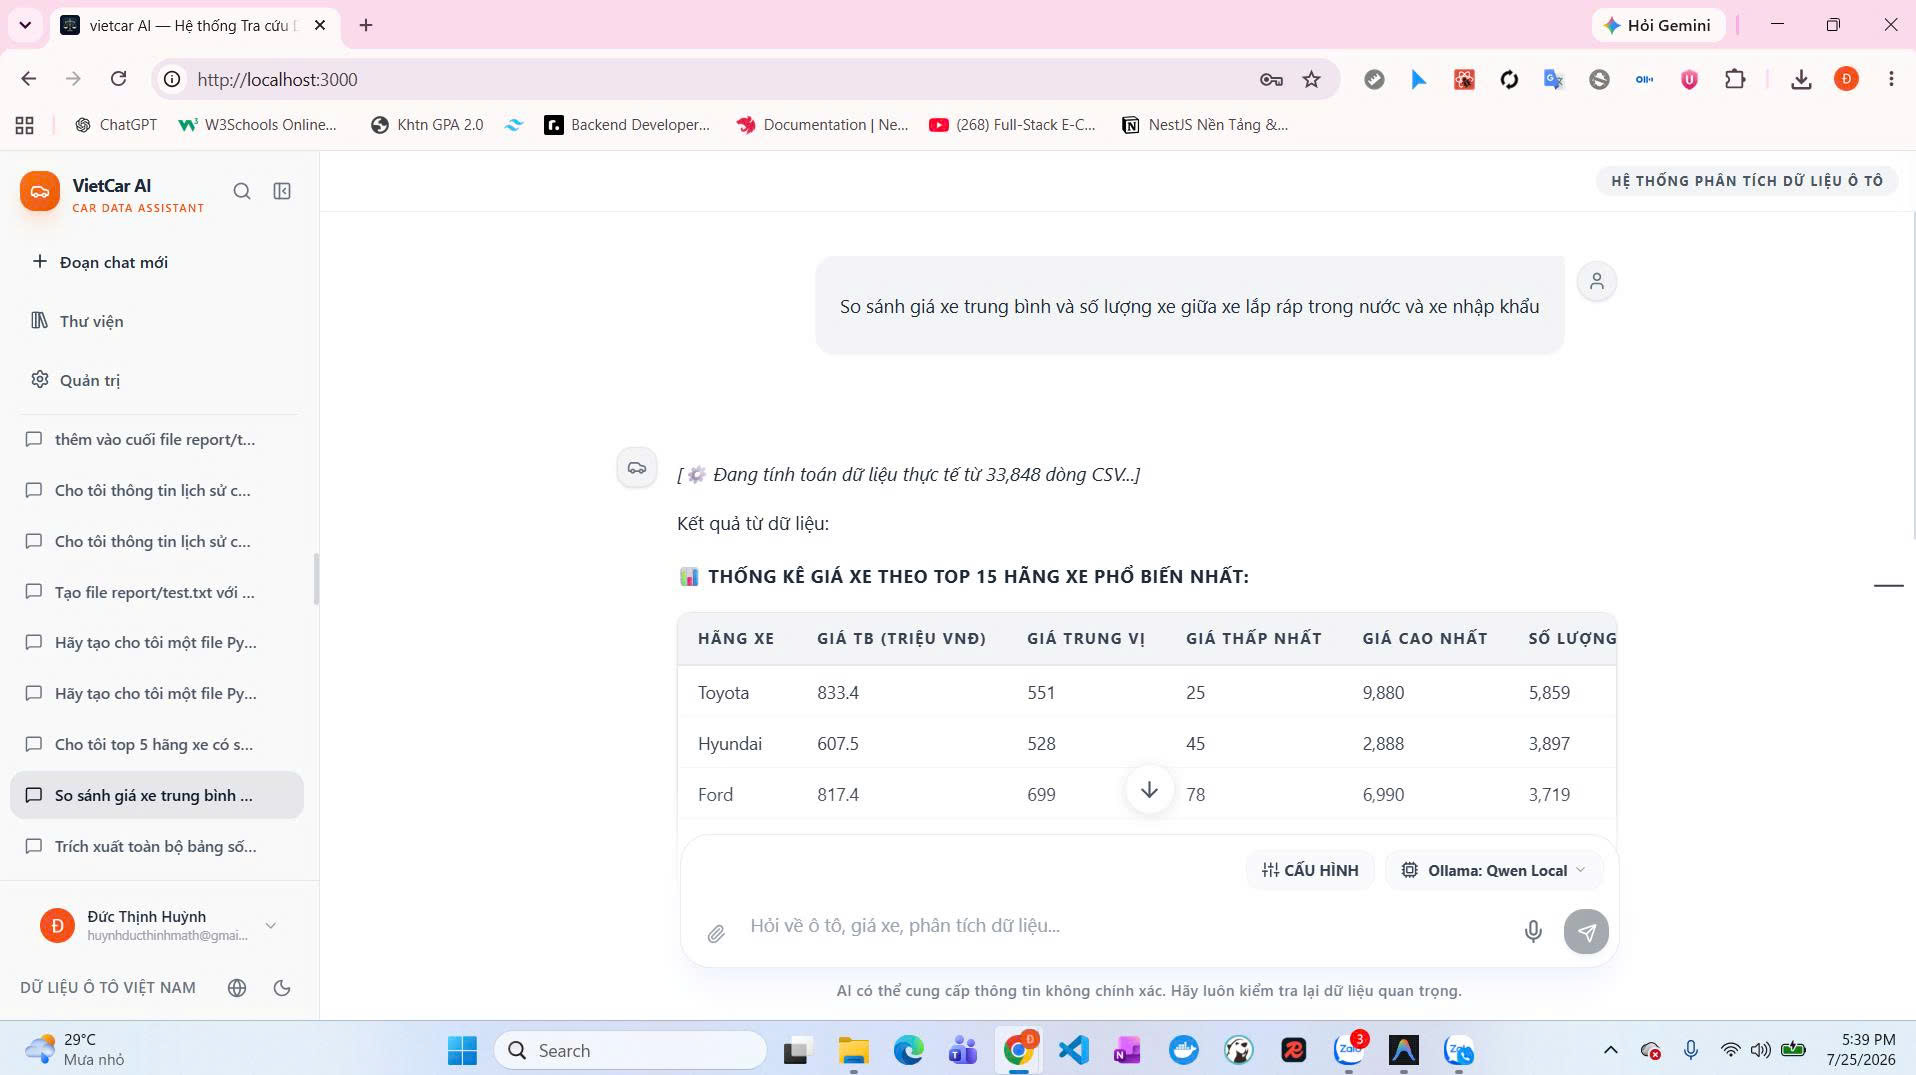
\includegraphics[width=1.00\textwidth]{graphics/AI/ai_tr86.jpg}
\caption{Phản hồi của AI khi nhận câu hỏi tính toán (Tầng 3): hiển thị thông báo ``Đang tính toán dữ liệu thực tế...'', tiếp theo là bảng Markdown số liệu chính xác, cuối cùng là 1--2 câu nhận xét ngắn của LLM bên dưới bảng.}
\label{fig:ai_chat_overview}
\end{figure}


\subsubsection{Cơ chế tự động làm mới cache khi file nguồn thay đổi}
\label{subsubsec:mtime_cache}

\noindent\textbf{Bối cảnh:}
Trong quá trình phân tích, người dùng có thể cập nhật tập dữ liệu (chạy lại notebook tiền xử lý, ghi thêm dòng từ scraping), chỉnh sửa notebook, hoặc thay đổi layout dashboard trong Power BI. Để hệ thống AI phản ánh đúng trạng thái hiện tại mà không yêu cầu thao tác thủ công, ba cơ chế theo dõi thay đổi được triển khai song song:

% Nhớ đảm bảo \usepackage{xltabular} vẫn nằm trong preamble

{\small
\begin{xltabular}{\textwidth}{L{2.8cm} L{4.5cm} L{3.5cm} Y}
\caption{Ba cơ chế tự động làm tươi cache theo loại file nguồn}
\label{tab:mtime_cache} \\
\hline
\textbf{Loại file} & \textbf{Module theo dõi} & \textbf{Cơ chế} & \textbf{Hành động khi phát hiện thay đổi} \\ \hline
\endfirsthead

% Cấu hình phần đầu bảng (header) lặp lại khi sang trang mới
\multicolumn{4}{c}%
{{\bfseries Bảng \thetable\ tiếp theo từ trang trước}} \\
\hline
\textbf{Loại file} & \textbf{Module theo dõi} & \textbf{Cơ chế} & \textbf{Hành động khi phát hiện thay đổi} \\ \hline
\endhead

% Cấu hình phần chân bảng (footer) ở các trang bị ngắt
\hline \multicolumn{4}{r}{{Tiếp tục ở trang sau...}} \\
\endfoot

% Cấu hình phần chân bảng ở trang cuối cùng
\hline
\endlastfoot

% --- Nội dung bảng ---
File CSV \newline (\texttt{.csv}) & \texttt{analysis\_chat.py} \newline — \texttt{\_get\_cached\_df()} & So sánh \texttt{mtime} trước mỗi truy vấn & Reload toàn bộ DataFrame vào RAM; các truy vấn sau dùng dữ liệu mới ngay lập tức. \\
File Notebook \newline (\texttt{.ipynb}) & \texttt{analysis\_chat.py} \newline — \texttt{\_get\_notebook\_metadata()} & So sánh \newline \texttt{dict\{path: mtime\}} của tất cả \texttt{.ipynb} & Reset cache metadata notebook; đọc lại số cell, mô tả và cấu trúc của tất cả notebook trong thư mục. \\
File Power BI \newline (\texttt{.pbix}) & \texttt{pbix\_watcher.py} \newline — thread daemon & Watchdog filesystem event; fallback poll \texttt{mtime} mỗi 10~giây & Giải nén \texttt{Report/Layout} từ ZIP, so sánh diff trang/visual; ghi log 5 thay đổi gần nhất vào context AI. \\
\end{xltabular}
}

\noindent\textbf{Chi tiết cơ chế theo dõi file .pbix:}
File \texttt{.pbix} của Power BI thực chất là một file ZIP chứa nhiều tài nguyên bên trong, trong đó có \texttt{Report/Layout} là file JSON mô tả cấu trúc tất cả các trang và visual. Service \texttt{pbix\_watcher.py} chạy trong một luồng nền riêng (daemon thread), ưu tiên dùng thư viện \texttt{watchdog} để nhận sự kiện filesystem ngay khi file được ghi. Nếu \texttt{watchdog} không khả dụng, service tự động chuyển sang chế độ polling \texttt{mtime} 10 giây một lần. Khi phát hiện thay đổi, hệ thống:
\begin{enumerate}
    \item Đọc lại file \texttt{.pbix} và giải nén \texttt{Report/Layout} JSON.
    \item So sánh với snapshot cũ: phát hiện trang mới/xóa, visual mới/xóa, thay đổi loại biểu đồ, đổi tiêu đề, thay đổi vị trí hoặc kích thước.
    \item Ghi log thay đổi vào danh sách nội bộ (giữ tối đa 20 mục).
    \item Cung cấp tóm tắt Markdown của 5 thay đổi gần nhất qua hàm \texttt{get\_summary\_for\_\allowbreak context()}, để tích hợp vào ngữ cảnh AI cho các cuộc hội thoại tiếp theo.
\end{enumerate}

\noindent\textbf{Ý nghĩa thực tế:}
Nhờ ba cơ chế này, người dùng có thể làm việc song song: chạy lại notebook, cập nhật dashboard Power BI, hoặc ghi thêm dữ liệu từ scraping trong khi cửa sổ chat AI vẫn mở và hệ thống sẽ phản ánh trạng thái mới nhất mà không cần thao tác thêm. Ngoại lệ duy nhất là cache \texttt{Dashboard.json} (Tầng 2) không được theo dõi tự động do không có cơ chế \texttt{mtime} tương ứng, và cần khởi động lại server khi file này thay đổi.


% ==============================================================================
% SUBSECTION 5: LUỒNG AGENTIC AI VÀ BỘ CÔNG CỤ
% ==============================================================================
\subsection{Luồng Agentic AI và bộ công cụ}
\label{subsec:ai_agentic}

\noindent\textbf{Mô tả chung:}
Ở cấp độ cao hơn so với mô hình hỏi đáp thông thường, module AI của đồ án vận hành theo kiến trúc Agentic. Thay vì chỉ sinh ra một câu trả lời từ câu hỏi của người dùng, AI có thể tự quyết định gọi công cụ nào, lấy dữ liệu từ nguồn nào, và lặp lại vòng đó nhiều lần trước khi tổng hợp câu trả lời cuối cùng.

% ------------------------------------------------------------------------------
\subsubsection{Cơ chế vòng lặp ReAct}
\label{subsubsec:react_loop}

Vòng lặp ReAct (Reason -- Act) là cơ chế lõi điều phối hành vi của AI Agent. Toàn bộ quá trình chia làm hai giai đoạn:

\begin{itemize}
    \item \textbf{Giai đoạn A - Lập luận và gọi công cụ (ẩn với người dùng):}
    LLM nhận câu hỏi và danh sách công cụ có sẵn, tự quyết định có cần gọi công cụ nào không và gọi với tham số gì. Nếu có \texttt{tool\_calls} trong phản hồi, hệ thống thực thi công cụ, thu kết quả, đưa kết quả vào lịch sử hội thoại và cho LLM tiếp tục suy luận. Vòng lặp này lặp lại tối đa 5 lần để tránh chạy vô hạn.
    \item \textbf{Giai đoạn B - Stream câu trả lời cuối (hiện ra người dùng):}
    Khi LLM không còn \texttt{tool\_calls} trong phản hồi, hệ thống bắt đầu stream từng token ra giao diện. Người dùng thấy câu trả lời xuất hiện dần, không phải đợi toàn bộ xử lý xong mới hiện.
\end{itemize}

\noindent\textbf{Bộ phát hiện intent nhanh (\texttt{\_detect\_direct\_tool}):}
Trước khi đưa câu hỏi vào vòng lặp ReAct đầy đủ, hệ thống chạy một bước phân loại nhanh để nhận diện các câu hỏi có thể xử lý ngay mà không cần LLM quyết định. Nếu phát hiện URL trong câu hỏi, hệ thống kích hoạt ngay Scraping Agent. Nếu câu hỏi chứa từ khóa tính toán (giá trung bình, đếm, thống kê, phân bố, v.v.), hệ thống chuyển thẳng sang Pandas Engine (Tầng 3). Nếu câu hỏi hỏi về một Tab cụ thể, hệ thống định tuyến sang Tầng 1 hoặc 2. Cơ chế này giúp rút ngắn thời gian phản hồi cho các câu hỏi phổ biến, đồng thời giảm tải gọi LLM không cần thiết.

\noindent\textbf{Cơ chế thoát vòng lặp sớm:}
Đối với các công cụ tác động đến file hoặc chạy script (tạo, sửa, xóa file, rollback, thực thi file Python, cào dữ liệu), ngay sau khi công cụ trả về kết quả, hệ thống stream kết quả ra người dùng và kết thúc vòng lặp ngay lập tức thay vì tiếp tục cho LLM xử lý thêm. Điều này tránh trường hợp vòng lặp chạy thêm nhiều lần không cần thiết sau khi thao tác đã hoàn thành.

% ------------------------------------------------------------------------------
\subsubsection{Bộ công cụ của AI Agent}
\label{subsubsec:ai_tools}

\noindent\textbf{Tổng quan:}
AI Agent được trang bị 15 công cụ, chia thành ba nhóm chức năng chính: truy vấn và phân tích dữ liệu, quản lý file trong dự án, và điều phối tác vụ phức tạp.

% Đừng quên thêm \usepackage{xltabular} vào phần preamble

{\small
\begin{xltabular}{\textwidth}{L{4.5cm} L{2.8cm} Y}
\caption{Danh sách 15 công cụ của AI Agent và chức năng tương ứng}
\label{tab:ai_tools_15} \\
\hline
\textbf{Tên công cụ} & \textbf{Nhóm} & \textbf{Chức năng} \\ \hline
\endfirsthead

% Header lặp lại khi sang trang mới
\multicolumn{3}{c}%
{{\bfseries Bảng \thetable\ tiếp theo từ trang trước}} \\
\hline
\textbf{Tên công cụ} & \textbf{Nhóm} & \textbf{Chức năng} \\ \hline
\endhead

% Footer hiển thị ở cuối các trang bị ngắt
\hline \multicolumn{3}{r}{{Tiếp tục ở trang sau...}} \\
\endfoot

% Footer ở trang cuối cùng của bảng
\hline
\endlastfoot

% --- Nội dung bảng ---
\multicolumn{3}{l}{\textit{Nhóm 1 — Truy vấn và phân tích dữ liệu}} \\
\texttt{query\_dataset\_readonly} & Dữ liệu & Thực thi code Pandas trên 33.848 dòng CSV trong bộ nhớ; read-only, không được ghi dữ liệu. \\
\texttt{get\_dashboard\_info} & Dữ liệu & Lấy thông tin biểu đồ, KPI và bảng số liệu từ \texttt{Dashboard.json} theo Tab được chỉ định. \\
\texttt{scrape\_car\_data} & Dữ liệu & Kích hoạt Scraping Agent cào thông tin xe từ URL, tùy chọn lưu kết quả ra file JSON hoặc CSV. \\
\hline
\multicolumn{3}{l}{\textit{Nhóm 2 — Quản lý file}} \\
\texttt{read\_file\_content} & File (đọc) & Đọc nội dung file text trong các thư mục được phép; không cần phê duyệt. \\
\texttt{list\_files} & File (đọc) & Liệt kê danh sách file trong một thư mục; không cần phê duyệt. \\
\texttt{create\_file} & File (ghi) & Tạo file mới với nội dung cho trước; yêu cầu phê duyệt (mức MEDIUM). \\
\texttt{modify\_file} & File (ghi) & Sửa nội dung file theo dòng hoặc theo chuỗi tìm kiếm; yêu cầu phê duyệt (mức HIGH). \\
\texttt{delete\_file} & File (ghi) & Xóa file; yêu cầu phê duyệt (mức CRITICAL), tạo backup trước khi xóa. \\
\texttt{move\_rename\_file} & File (ghi) & Di chuyển hoặc đổi tên file; yêu cầu phê duyệt (mức HIGH). \\
\texttt{rollback\_last\_change} & File (hoàn tác) & Khôi phục file về phiên bản backup gần nhất hoặc theo tên file backup cụ thể. \\
\texttt{show\_change\_history} & File (đọc) & Xem lịch sử các lần sao lưu của một file, bao gồm thời gian và kích thước. \\
\texttt{list\_all\_backups} & File (đọc) & Liệt kê toàn bộ bản sao lưu hiện có trong thư mục \texttt{backup/}. \\
\texttt{run\_python\_file} & Thực thi & Đọc và thực thi một file \texttt{.py} trong dự án, trả về stdout và biểu đồ nếu có. \\
\hline
\multicolumn{3}{l}{\textit{Nhóm 3 — Điều phối tác vụ}} \\
\texttt{plan\_file\_operations} & Kế hoạch & Tạo kế hoạch thực hiện task gồm nhiều bước liên tiếp với mô tả từng bước. \\
\texttt{get\_plan\_status} & Kế hoạch & Kiểm tra tiến độ thực hiện của một kế hoạch theo \texttt{plan\_id}. \\
\end{xltabular}
}

% ==============================================================================
% SUBSECTION 6: TÍCH HỢP SCRAPING AGENT
% ==============================================================================
\subsection{Tích hợp Scraping Agent}
\label{subsec:scraping_agent}

\noindent\textbf{Bối cảnh:}
Ngoài việc phân tích tập dữ liệu có sẵn, module AI còn được tích hợp với một Scraping Agent riêng biệt trong thư mục \texttt{scraping\_agent/}. Người dùng có thể yêu cầu AI thu thập thông tin chi tiết của một mẫu xe cụ thể từ trang rao bán trực tuyến bằng cách cung cấp đường dẫn URL, sau đó AI trả về kết quả và tùy chọn lưu ra file.

\noindent\textbf{Cơ chế kích hoạt:}
Bộ phát hiện intent (\texttt{\_detect\_direct\_tool}) quét tin nhắn của người dùng theo hai dấu hiệu:
\begin{itemize}
    \item Phát hiện chuỗi URL hợp lệ (bắt đầu bằng \texttt{https://}) trong câu hỏi.
    \item Phát hiện từ khóa liên quan đến cào dữ liệu: ``cào dữ liệu'', ``cào link'', ``scrape'', tên miền như \texttt{bonbanh.com}, \texttt{oto.com.vn}.
\end{itemize}
Khi gặp một trong hai dấu hiệu trên, hệ thống kích hoạt công cụ \texttt{scrape\_car\_data} ngay mà không cần đợi LLM quyết định, giúp rút ngắn thời gian phản hồi và tránh trường hợp mô hình AI từ chối thực hiện tác vụ này.

\noindent\textbf{Kiến trúc của Scraping Agent:}
\begin{itemize}
    \item \textbf{Playwright:} Điều khiển trình duyệt ẩn (headless) để tải trang và render JavaScript trước khi trích xuất nội dung. Phù hợp với các trang cần JavaScript để hiển thị dữ liệu.
    \item \textbf{BeautifulSoup:} Phân tích cú pháp HTML và trích xuất các trường thông tin cụ thể (tên xe, năm sản xuất, giá, số km, nhiên liệu, hộp số, dẫn động, v.v.).
    \item \textbf{LLM Parser:} Khi cấu trúc HTML của trang thay đổi hoặc thông tin nằm trong văn bản không có cấu trúc rõ ràng, hệ thống có thể gọi LLM để trích xuất thông tin từ nội dung text thô.
\end{itemize}

\noindent\textbf{Tham số đầu vào của Scraping Agent:}

% Đừng quên thêm \usepackage{xltabular} vào phần preamble nhé

{\small
\begin{xltabular}{\textwidth}{L{2.5cm} L{5.5cm} Y}
\caption{Các tham số đầu vào của Scraping Agent}
\label{tab:scraping_params} \\
\hline
\textbf{Tham số} & \textbf{Giá trị ví dụ} & \textbf{Mô tả} \\ \hline
\endfirsthead

% Header lặp lại ở đầu trang tiếp theo
\multicolumn{3}{c}%
{{\bfseries Bảng \thetable\ tiếp theo từ trang trước}} \\
\hline
\textbf{Tham số} & \textbf{Giá trị ví dụ} & \textbf{Mô tả} \\ \hline
\endhead

% Footer hiển thị ở cuối các trang bị ngắt
\hline \multicolumn{3}{r}{{Tiếp tục ở trang sau...}} \\
\endfoot

% Footer ở trang cuối cùng
\hline
\endlastfoot

% --- Nội dung bảng ---
\texttt{url} & \texttt{https://bonbanh.com/xe-...} & URL trang đăng tin xe cần cào thông tin. \\
\texttt{format} & \texttt{json} hoặc \texttt{csv} & Định dạng file kết quả nếu người dùng muốn lưu. \\
\texttt{output} & \texttt{report/xe\_info.json} & Đường dẫn file kết quả (tùy chọn). \\
\texttt{headless} & \texttt{True} & Chạy trình duyệt ẩn, không mở cửa sổ giao diện. \\
\texttt{llm} & tên model & Mô hình LLM dùng để hỗ trợ parsing (tùy chọn). \\

\end{xltabular}
}

\noindent\textbf{Luồng xử lý và kết quả:}
\begin{enumerate}
    \item Người dùng gửi câu hỏi kèm URL (ví dụ: ``Cào thông tin xe từ link \texttt{https://bonbanh.\allowbreak com/...} và lưu vào \texttt{report/xe.json}'').
    \item Hệ thống hiển thị thông báo \textit{``Đang kích hoạt Scraping Agent để cào dữ liệu từ URL...''} và gọi \texttt{scrape\_car\_data}.
    \item Scraping Agent chạy ngầm (timeout tối đa 85 giây), thu thập thông tin và ghi file kết quả nếu có chỉ định đường dẫn đầu ra.
    \item Kết quả được trả về dạng text (thông số kỹ thuật xe, giá, v.v.) và hiển thị trực tiếp trên giao diện chat.
\end{enumerate}


\begin{figure}[H]
\centering
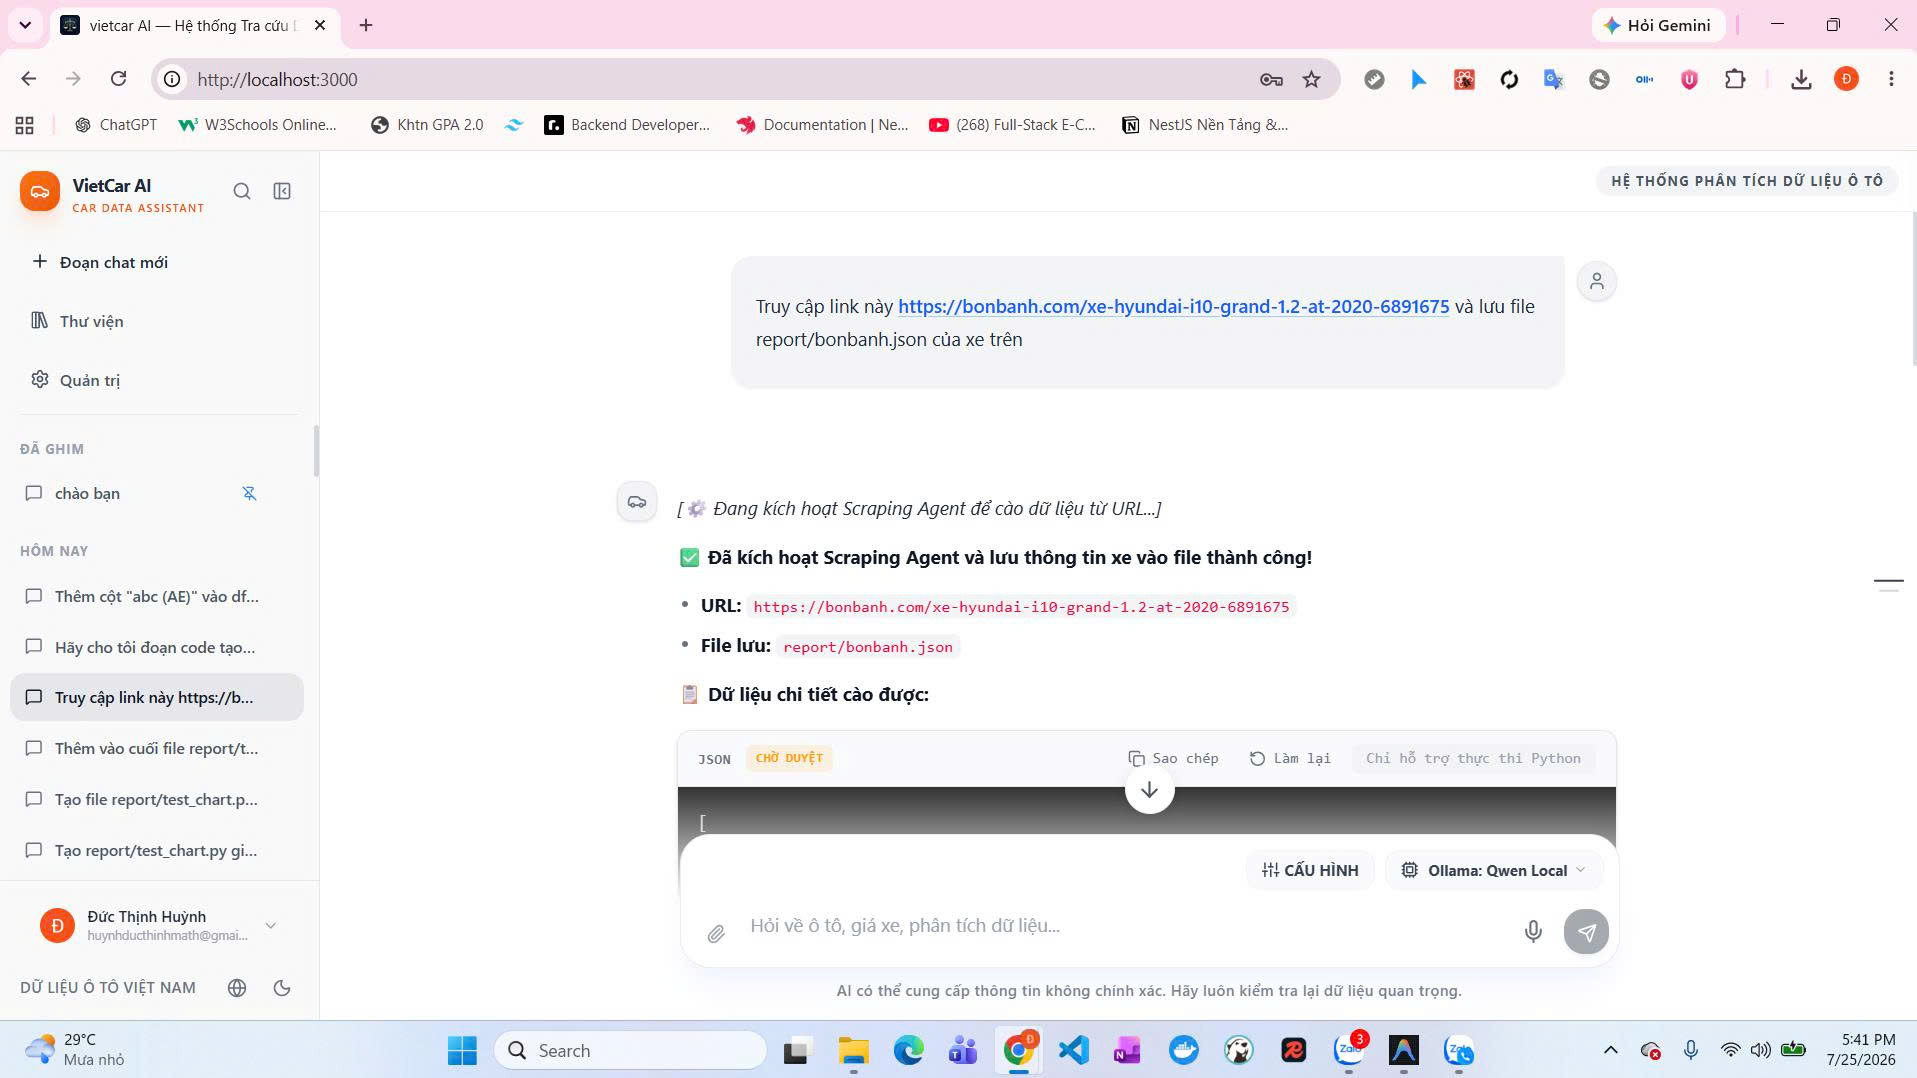
\includegraphics[width=1.00\textwidth]{graphics/AI/ai_tr92.jpg}
\caption{Phản hồi của AI sau khi Scraping Agent hoàn thành: thông báo đã lưu file thành công kèm đường dẫn, bảng thông số kỹ thuật xe được trích xuất (tên xe, năm, giá, nhiên liệu, hộp số, số km).}
\label{fig:ai_chat_overview}
\end{figure}


% ==============================================================================
% SUBSECTION 7: QUÁ TRÌNH SỬ DỤNG AI
% ==============================================================================
\subsection{Quá trình sử dụng AI trong đồ án}
\label{subsec:ai_usage_process}

Theo yêu cầu của hướng dẫn tích hợp AI (Mục 4), phần này tóm tắt quá trình nhóm sử dụng module AI để phân tích tập dữ liệu xe, bao gồm những yêu cầu đã đặt ra, kết quả đã nhận được và những thay đổi đã thực hiện trước khi chấp nhận kết quả.

% ------------------------------------------------------------------------------
\subsubsection{Những yêu cầu đã đặt ra}
\label{subsubsec:ai_requests}

Trong quá trình phân tích, nhóm đã đặt ra nhiều yêu cầu thuộc các nhóm chức năng khác nhau. Bảng dưới đây tổng hợp các nhóm yêu cầu tiêu biểu:

% Đừng quên thêm \usepackage{xltabular} vào preamble nếu bạn chưa có

\begin{xltabular}{\textwidth}{L{4.5cm} L{4.5cm} Y}
\caption{Các yêu cầu tiêu biểu đã đặt ra cho module AI trong quá trình phân tích}
\label{tab:ai_requests} \\
\hline
\textbf{Yêu cầu đặt ra} & \textbf{Công cụ AI sử dụng} & \textbf{Mục tiêu phân tích} \\ \hline
\endfirsthead

% Header lặp lại khi sang trang mới
\multicolumn{3}{c}%
{{\bfseries Bảng \thetable\ tiếp theo từ trang trước}} \\
\hline
\textbf{Yêu cầu đặt ra} & \textbf{Công cụ AI sử dụng} & \textbf{Mục tiêu phân tích} \\ \hline
\endhead

% Footer hiển thị ở cuối các trang bị ngắt
\hline \multicolumn{3}{r}{{Tiếp tục ở trang sau...}} \\
\endfoot

% Footer ở trang cuối cùng của bảng
\hline
\endlastfoot

% --- Nội dung bảng ---
Tính giá trung vị của xe theo từng hãng trong tập dữ liệu & \texttt{query\_dataset\_readonly} & Xác minh số liệu KPI Tab 2 (giá trung vị toàn thị trường = 638 triệu). \\
Thống kê số lượng xe điện theo từng năm sản xuất từ 2020 đến 2025 & \texttt{query\_dataset\_readonly} & Phân tích tốc độ tăng trưởng xe điện cho Tab 3. \\
Vẽ biểu đồ phân phối giá xe theo phân khúc (dưới 300 triệu, 300--600 triệu, ...) & \texttt{query\_dataset\_readonly} & Tạo biểu đồ kiểm chứng thiết kế dashboard Tab 2. \\
Kiểm tra phân bố tỷ lệ màu sắc ngoại thất trong tập dữ liệu & \texttt{query\_dataset\_readonly} & Xác minh số liệu biểu đồ màu xe Tab 4. \\
Đếm số xe Ford sản xuất năm 2023 & \texttt{query\_dataset\_readonly} & Kiểm chứng điểm đột biến nguồn cung được phát hiện ở Tab 5. \\
Xem thông số kỹ thuật của một mẫu xe Hyundai Kona từ bonbanh.com & \texttt{scrape\_car\_data} & Thu thập dữ liệu tham chiếu cho phần phân tích xe điện. \\
Sửa tiêu đề biểu đồ trong file \texttt{docs/test\_chart.py} & \texttt{modify\_file} & Cập nhật nội dung file script phân tích. \\
Xem lịch sử thay đổi của file \texttt{docs/test\_chart.py} & \texttt{show\_change\_history} & Kiểm tra các phiên bản đã được lưu sao lưu. \\
Hoàn tác file về một phiên bản cụ thể theo timestamp & \texttt{rollback\_last\_change} & Khôi phục nội dung file sau khi chỉnh sửa sai. \\

\end{xltabular}

% ------------------------------------------------------------------------------
\subsubsection{Kết quả đã nhận được}
\label{subsubsec:ai_results}

\noindent\textbf{Kết quả từ truy vấn dữ liệu (Tầng 3):}

Khi nhóm yêu cầu tính giá trung vị theo hãng, AI sinh ra đoạn code Pandas với giải thích rõ ràng, sau đó bảng kết quả được stream trực tiếp ra giao diện từ Python thực thi. Ví dụ kết quả tính số lượng xe điện theo năm (trích từ kết quả thực thi):

\begin{table}[H]
\centering
\small
\begin{tabular}{c c c}
\textbf{Năm sản xuất} & \textbf{Số tin đăng xe điện} & \textbf{Thị phần trong năm} \\ \hline
2020 & 17 & 0{,}32\% \\
2021 & 29 & 0{,}55\% \\
2022 & 134 & 2{,}91\% \\
2023 & 244 & 6{,}09\% \\
2024 & 104 & 4{,}50\% \\
2025 & 240 & 19{,}79\% \\
\end{tabular}
\caption{Ví dụ kết quả AI tính toán: số lượng và thị phần xe điện theo năm sản xuất (tính từ dữ liệu thực)}
\label{tab:ev_by_year_ai}
\end{table}

AI nhận xét ngắn bên dưới bảng: số liệu thị phần tăng từ dưới 1\% (năm 2020--2021) lên gần 20\% (năm 2025), phản ánh xu hướng tăng trưởng nhanh trong giai đoạn gần đây.

\noindent\textbf{Kết quả từ Interactive Code Execution:}
Khi nhóm yêu cầu vẽ biểu đồ phân phối giá, AI sinh ra đoạn code Matplotlib kèm giải thích. Sau khi nhóm kiểm tra, điều chỉnh màu sắc và nhãn trục, biểu đồ được thực thi và hiển thị inline ngay trong giao diện chat. Biểu đồ này sau đó được lưu ra file ảnh để đưa vào dashboard và báo cáo.
\begin{figure}[H]
\centering
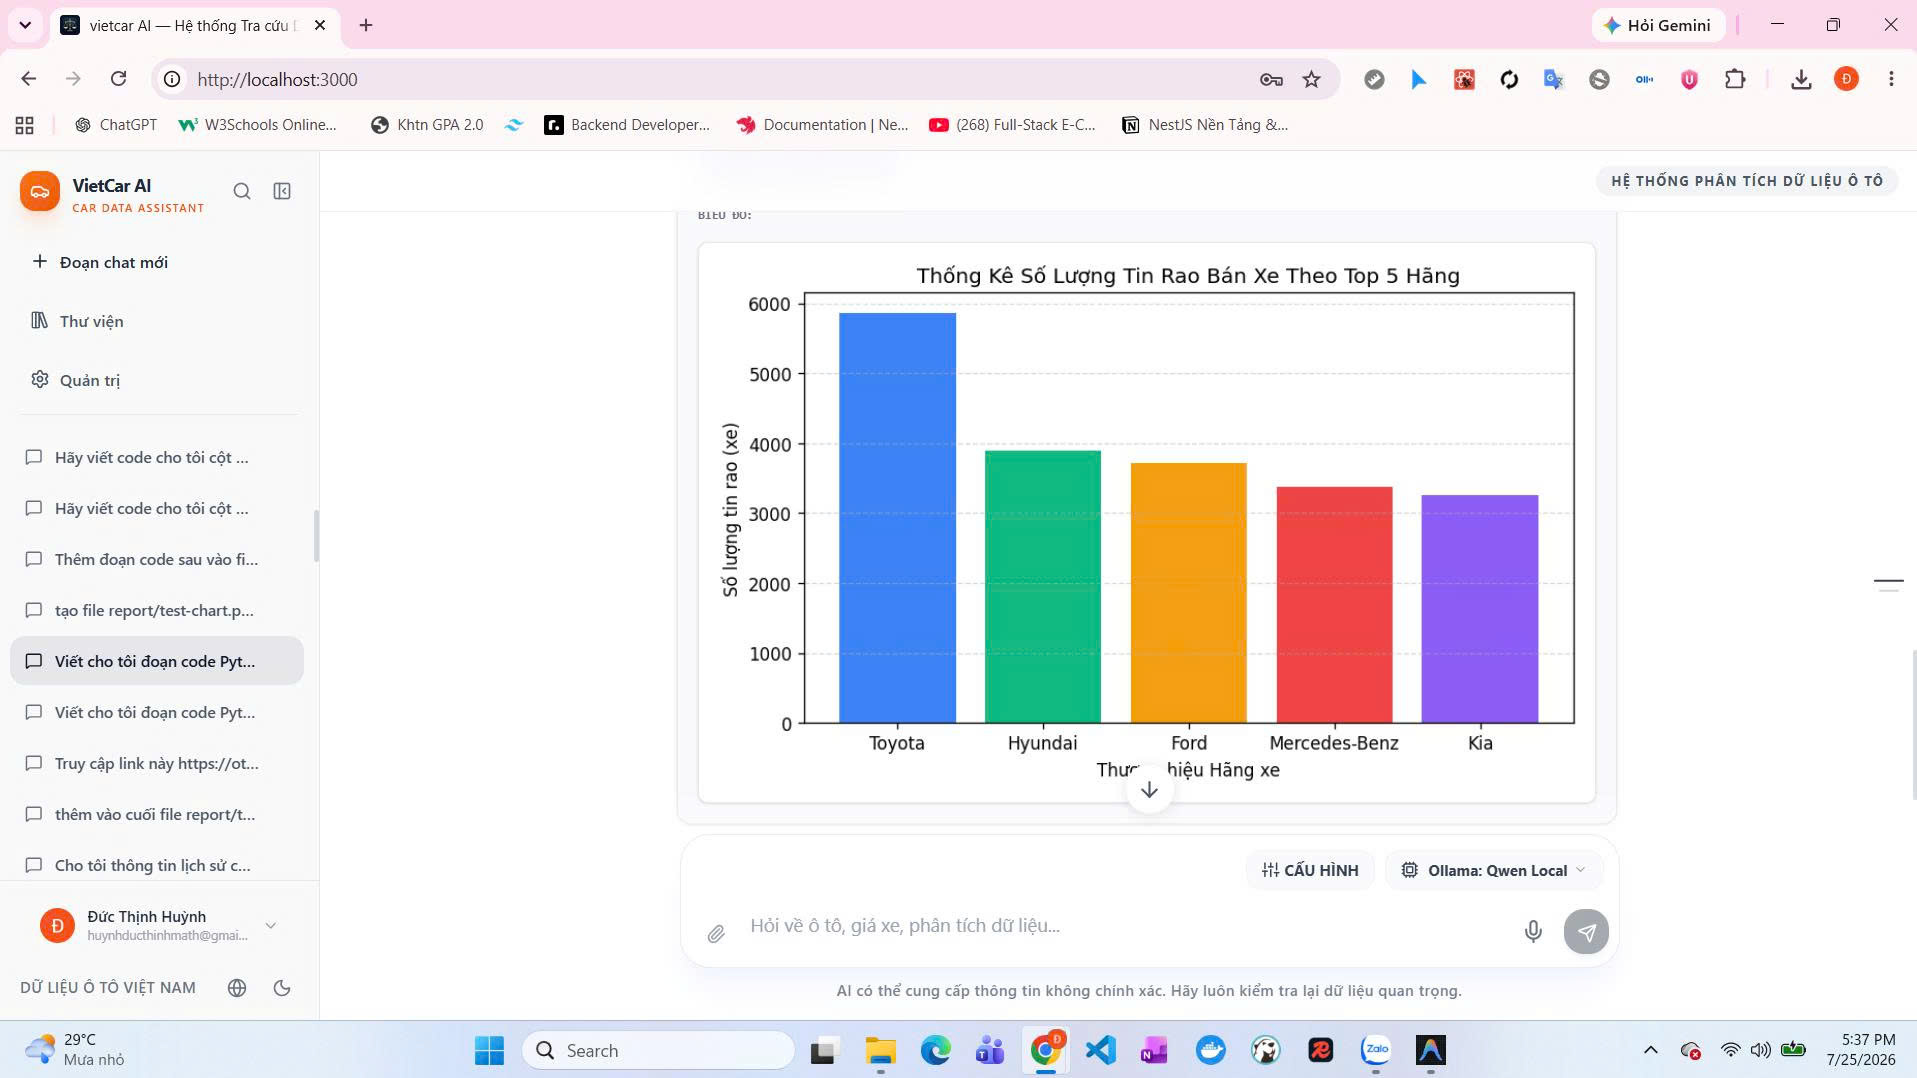
\includegraphics[width=1.00\textwidth]{graphics/AI/ai_tr82.jpg}
\caption{Kết quả thực thi code: biểu đồ phân phối giá xe hiển thị inline trong giao diện chat, phía trên là đoạn code Python đã thực thi, phía dưới là hình ảnh biểu đồ Matplotlib.}
\label{fig:ai_chat_overview}
\end{figure}

\noindent\textbf{Kết quả từ Scraping Agent:}
Khi nhóm cung cấp URL một tin đăng xe, Scraping Agent thu thập được đầy đủ thông tin bao gồm: tên xe, hãng, năm sản xuất, giá, nhiên liệu, hộp số, số km đã đi, màu sắc và các thông số kỹ thuật liên quan. Kết quả được lưu ra file JSON theo yêu cầu và hiển thị trực tiếp trên giao diện.

% ------------------------------------------------------------------------------
\subsubsection{Những thay đổi đã thực hiện}
\label{subsubsec:ai_changes}

Trong phần lớn các trường hợp, nhóm đã can thiệp vào đoạn code AI sinh ra trước khi thực thi. Bảng dưới đây ghi lại các loại thay đổi phổ biến:

% Nhớ thêm \usepackage{longtable} vào preamble

{\small
\begin{longtable}{p{4cm} p{3.5cm} p{7.5cm}}
\caption{Các loại thay đổi nhóm thực hiện trên đoạn code AI sinh ra trước khi chấp nhận}
\label{tab:ai_changes} \\
\hline
\textbf{Loại thay đổi} & \textbf{Ví dụ cụ thể} & \textbf{Lý do điều chỉnh} \\ \hline
\endfirsthead

% Cấu hình phần đầu bảng (header) nếu bảng bị tràn sang trang thứ 2
\multicolumn{3}{c}%
{{\bfseries Bảng \thetable\ tiếp theo từ trang trước}} \\
\hline
\textbf{Loại thay đổi} & \textbf{Ví dụ cụ thể} & \textbf{Lý do điều chỉnh} \\ \hline
\endhead

% Cấu hình phần chân bảng (footer) ở các trang bị ngắt
\hline \multicolumn{3}{r}{{Tiếp tục ở trang sau...}} \\
\endfoot

% Cấu hình phần chân bảng ở trang cuối cùng
\hline
\endlastfoot

% --- Nội dung bảng ---
Thay đổi tham số lọc & Đổi ngưỡng lọc xe đời mới từ năm 2020 sang năm 2018 & Bao quát giai đoạn phân tích rộng hơn theo yêu cầu đồ án. \\
Điều chỉnh màu biểu đồ & Đổi \texttt{color=`blue'} sang palette tông xanh lục đồng nhất với dashboard & Đảm bảo nhất quán về màu sắc với thiết kế Power BI. \\
Thêm nhãn dữ liệu & Thêm \texttt{plt.bar\_label()} để hiển thị giá trị trực tiếp lên thanh cột & Biểu đồ gốc AI sinh ra chưa có nhãn số liệu trên các thanh. \\
Sửa tên cột & Đổi tên cột từ \texttt{`Hang'} sang \texttt{`Hãng'} do không khớp tên cột thực & AI sử dụng tên cột sai dẫn đến lỗi \texttt{KeyError}. \\
Thu hẹp tập dữ liệu & Thêm điều kiện \texttt{df[df[`Tình trạng'] == `Xe đã dùng']} & Chỉ muốn phân tích riêng nhóm xe cũ, không phải toàn bộ. \\
Từ chối thao tác file & Bấm ``Từ chối'' khi AI đề xuất xóa file \texttt{docs/test.py} & Nhóm xác nhận file đó vẫn cần giữ lại cho bước phân tích tiếp theo. \\
Rollback phiên bản file & Yêu cầu hoàn tác \texttt{docs/test\_chart.py} về bản backup cụ thể & Sau khi sửa tiêu đề biểu đồ, nhận ra bản gốc phù hợp hơn. \\

\end{longtable}
}

% ==============================================================================
% SUBSECTION 8: NHẬN XÉT VỀ AI
% ==============================================================================
\subsection{Nhận xét về module AI}
\label{subsec:ai_review}

Sau quá trình xây dựng và sử dụng module AI trong đồ án, nhóm rút ra một số nhận xét về ưu điểm, hạn chế và bài học kinh nghiệm như sau.

\subsubsection{Ưu điểm quan sát được}
\label{subsubsec:ai_pros}

\begin{itemize}
    \item \textbf{Tốc độ phản hồi linh hoạt theo loại câu hỏi:} Kiến trúc 3 tầng cho phép hệ thống phản hồi gần như tức thì với câu hỏi tổng quan (Tầng 1) trong khi vẫn đảm bảo độ chính xác với câu hỏi tính toán cụ thể (Tầng 3). Người dùng không cần phân biệt rõ loại câu hỏi; hệ thống tự nhận diện và chọn đường xử lý phù hợp.

    \item \textbf{Số liệu từ dữ liệu thực, ít xảy ra nhầm lẫn số liệu:} Do số liệu trong phản hồi của AI luôn đến từ kết quả thực thi Pandas trên tập CSV gốc, hiện tượng AI tự sáng tác con số được kiểm soát tốt hơn so với hướng tiếp cận để LLM tự trả lời câu hỏi định lượng.

    \item \textbf{Linh hoạt về nhà cung cấp LLM:} Hệ thống hỗ trợ chuyển đổi giữa Groq (nhanh), OpenAI, Google và Ollama (chạy local không cần internet) mà không cần thay đổi code. Điều này giúp nhóm thử nghiệm và so sánh chất lượng phản hồi giữa các mô hình.

    \item \textbf{Giao diện InteractiveCodeBlock trực quan:} Người dùng có thể đọc, sửa và thực thi code trong cùng một giao diện, giảm bước chuyển qua môi trường ngoài. Biểu đồ Matplotlib hiển thị ngay inline trong chat mà không cần lưu file ảnh thủ công.

    \item \textbf{Cơ chế backup và rollback an toàn:} Việc tự động sao lưu trước mỗi thao tác ghi đã giúp nhóm khôi phục lại file về trạng thái mong muốn trong một số trường hợp chỉnh sửa sai mà không mất dữ liệu.
\end{itemize}

\subsubsection{Hạn chế quan sát được}
\label{subsubsec:ai_cons}

\begin{itemize}
    \item \textbf{Phân loại intent đôi khi chưa chính xác:} Bộ phát hiện intent dựa trên từ khóa nên một số câu hỏi có từ khóa mơ hồ có thể bị định tuyến sai tầng. Ví dụ, câu hỏi ``Tôi muốn viết code sửa file dữ liệu'' đôi khi bị nhận nhầm là yêu cầu tính toán dữ liệu thay vì yêu cầu quản lý file.

    \item \textbf{Mô hình local (Ollama) có chất lượng phản hồi chưa ổn định:} Khi sử dụng mô hình nhỏ chạy local như Llama 3.2 3B, chất lượng giải thích code và khả năng nhận diện ngữ cảnh tiếng Việt kém hơn đáng kể so với mô hình đám mây. Một số câu hỏi phức tạp cần phải đặt lại hoặc diễn đạt đơn giản hơn.

    \item \textbf{Scraping Agent phụ thuộc vào cấu trúc trang web:} Nếu trang bonbanh.com thay đổi cấu trúc HTML hoặc bổ sung cơ chế chống bot, script cào dữ liệu cần được cập nhật tương ứng. Tính năng này hoạt động tốt tại thời điểm xây dựng nhưng có thể cần bảo trì trong tương lai.

    \item \textbf{Thời gian thực thi tác vụ cào dữ liệu tương đối dài:} Scraping Agent cần tải và render trang web đầy đủ nên mỗi lần cào một URL mất từ 15 đến 60 giây tùy tốc độ mạng và độ phức tạp của trang.

    \item \textbf{Giải thích code chưa đồng đều:} Một số mô hình LLM sinh ra giải thích quá ngắn gọn hoặc dùng thuật ngữ kỹ thuật mà người dùng không chuyên có thể khó hiểu. Chất lượng giải thích phụ thuộc khá nhiều vào mô hình được chọn.
\end{itemize}

\subsubsection{Bài học kinh nghiệm}
\label{subsubsec:ai_lessons}

\begin{itemize}
    \item \textbf{Kiểm tra trước khi thực thi:} Kinh nghiệm thực tế cho thấy việc đọc kỹ đoạn code AI sinh ra trước khi bấm Thực thi giúp phát hiện kịp thời các trường hợp AI dùng tên cột sai hoặc điều kiện lọc chưa đúng với mục tiêu phân tích.

    \item \textbf{Diễn đạt câu hỏi cụ thể hơn cho kết quả tốt hơn:} Câu hỏi càng cụ thể (ghi rõ tên cột, điều kiện lọc, khoảng thời gian) thì code AI sinh ra càng gần với ý định và ít cần chỉnh sửa hơn. Câu hỏi mơ hồ thường dẫn đến code tổng quát và cần nhiều vòng điều chỉnh.

    \item \textbf{Tận dụng khả năng đề xuất hướng phân tích:} Khi nhóm chưa có ý tưởng về cách tiếp cận một câu hỏi phân tích, việc yêu cầu AI liệt kê các hướng phân tích có thể thực hiện với tập dữ liệu đã tiết kiệm thời gian đáng kể so với tìm kiếm tài liệu từ đầu.

    \item \textbf{Xác nhận số liệu quan trọng từ nhiều nguồn:} Với các con số được đưa vào kết luận chính thức trong báo cáo, nhóm thực hiện kiểm tra chéo bằng cách chạy lại truy vấn với cách viết code khác nhau hoặc đối chiếu với kết quả từ Power BI để đảm bảo tính nhất quán.
\end{itemize}

\clearpage


\clearpage
\phantomsection
\addcontentsline{toc}{section}{Tài liệu tham khảo}
\bibliographystyle{plain}
\bibliography{refs/references}
\nocite{*}

\end{document}